\documentclass[a4paper, openany, 12pt]{article}

%% подключаем стандарт библиографии
\bibliographystyle{gost71u}

%% для "Abstract" в классе book
% \newenvironment{abstract}{}{}
% \usepackage{abstract}

%% подключаем преамбулу: в ней содержится подключение всех необходимых пакетов
%% Работа с русским языком
\usepackage{cmap}			 % поиск в PDF
\usepackage{mathtext} 		 % русские буквы в формулах
\usepackage[T2A]{fontenc}	 % кодировка
\usepackage[utf8]{inputenc}	 % кодировка исходного текста
\usepackage[russian]{babel}	 % локализация и переносы

%% Пакеты для работы с математикой
\usepackage{amsmath,amsfonts,amssymb,amsthm,mathtools}
\usepackage{icomma}

%% Нумерация формул (опционально)
%\mathtoolsset{showonlyrefs=true} % показывать номера только у тех формул, на которые есть \eqref{} в тексте.
%\usepackage{leqno}               % нумерация формул слева

%% Шрифты
\usepackage{euscript}	 % шрифт "Евклид"
\usepackage{mathrsfs}    % красивый мат. шрифт

%% Некоторые полезные макросы для дебага (в случае недоверия авторам шаблона)
\makeatletter
\newcommand\thefontsize{The current font size is: \f@size pt} % пример: \section{\thefontsize}
\makeatother

%% Настройка размеров шрифтов
\makeatletter
\setlength{\headheight}{28pt}
%% TODO: мне не удалось разобраться, как грамотно подбирать второе число в 
%% \@setfontsize\*, но ряд эксппериментов показывает, что "10" выравнивает текст весьма прилично :)
\renewcommand\Huge{\@setfontsize\Huge{14pt}{10}}
\renewcommand\huge{\@setfontsize\huge{14pt}{10}}
\renewcommand\Large{\@setfontsize\Large{14pt}{10}}
\renewcommand\large{\@setfontsize\large{12pt}{10}}
\makeatother

%% Поля (геометрия страницы)
\usepackage[left=3cm,right=1.5cm,top=2cm,bottom=2cm,bindingoffset=0cm]{geometry}

%% Русские списки
\usepackage{enumitem}
\makeatletter
\AddEnumerateCounter{\asbuk}{\russian@alph}{щ}
\makeatother

%% Работа с картинками
\usepackage{caption}
\captionsetup{justification=centering} % центрирование подписей к картинкам
\usepackage{graphicx}                  % вставки рисунков
\graphicspath{{images/}{images2/}}     % папки с картинками
\setlength\fboxsep{3pt}                % отступ рамки \fbox{} от рисунка
\setlength\fboxrule{1pt}               % толщина линий рамки \fbox{}
\usepackage{wrapfig}                   % обтекание рисунков и таблиц текстом

%% Работа с таблицами
\usepackage{array,tabularx,tabulary,booktabs} % дополнительная работа с таблицами
\usepackage{longtable}                        % длинные таблицы
\usepackage{multirow}                         % слияние строк в таблице

%% Красная строка
\setlength{\parindent}{2em}

%% Интервалы
\linespread{1}
\usepackage{multirow}
\usepackage{graphicx}         % Работа с графикой
\usepackage{subcaption}    

%% TikZ
\usepackage{tikz}
\usetikzlibrary{graphs,graphs.standard}

%% Верхний колонтитул
\usepackage{fancyhdr}
\pagestyle{fancy}

%% Перенос знаков в формулах (по Львовскому)
\newcommand*{\hm}[1]{#1\nobreak\discretionary{}{\hbox{$\mathsurround=0pt #1$}}{}}

%% Дополнительно
\usepackage{float}   % добавляет возможность работы с командой [H] которая улучшает расположение на странице
\usepackage{gensymb} % красивые градусы
\usepackage{caption} % пакет для подписей к рисункам, в частности, для работы caption*
\usepackage{listings} % пакет для листингов с кодом
\lstset{              % настройки для лисингов с кодом
basicstyle=\small\ttfamily,
columns=flexible,
breaklines=true
}

% Hyperref (для ссылок внутри  pdf)
\usepackage[unicode, pdftex]{hyperref}

% Отступ перед первым абзацем в каждом разделе
\usepackage{indentfirst}


\begin{document}
    %% титульник
    \begin{center}
    %% *название института*
    \large\textbf{Министерство образования и науки Российской Федерации \\
        Московский физико-технический институт (государственный
        университет)} \\
    \vspace{1cm}

    %% *факультет/физтех-школа*
    Физтех-школа прикладной математики и информатики \\

    %% *название базовой кафедры и лаборатории*
    %% в случае ненадобности можно удалить
    Кафедра банковских информационных технологий \\

    \vspace{3em}

    Выпускная квалификационная работа бакалавра
\end{center}

\begin{center}
    \vspace{\fill}
    %% *название вашей работы*
    \LARGE{Разработка системы автоматизированного проектирования PointCloud2CAD}

    \vspace{\fill}
\end{center}

\begin{flushright}
    \textbf{Автор:} \\
    Студент Б05-103 группы \\
    Родригес Яновицкий Антонио Александрович \\
    \vspace{2em}
    \textbf{Научный руководитель:} \\
    Бочаров Иван Геннадьевич \\
    \vspace{2em}
    \textbf{Научный консультант:} \\
    Пасечник Игорь Игоревич \\
\end{flushright}

\vspace{7em}

\begin{center}
    %% *лого*
    \includegraphics[width=100 pt]{MIPT_logo.jpg}\\
    Москва \the\year{}
\end{center}

%% выключаем отображение номера для этой страницы (титульник)
\thispagestyle{empty}

\newpage
\setcounter{page}{2}
\fancyfoot[c]{\thepage}
%% *надпись над верхним колонтинулом*
%% в случае ненадобности можно удалить
\fancyhead[L]{Разработка системы автоматизированного проектирования PointCloud2CAD}
\fancyhead[R]{}
    %% аннотоция
    \begin{abstract}

    \begin{center}
        \large{Разработка системы автоматизированного проектирования PointCloud2CAD} \\
        \large\textit{} \\[1 cm]
    \end{center}
    % Краткое описание задачи и основных результатов, мотивирующее прочитать весь текст.

    \noindent Система автоматизированного проектирования (CAD) широко применяется в инженерной отрасли,
    однако реализация промышленных проектов в формате «end-to-end» зачастую оказывается крайне затратной и продолжительной по времени.
    Например, создание 3D-модели автомобиля методом реверс-инжиниринга из облака точек может растянуться на три месяца и потребовать вложений порядка полумиллиона.
    Дополнительным препятствием является нехватка в России квалифицированных специалистов по 3D-инжинирингу.
    Все эти факторы подчеркивают высокую актуальность задачи генерации CAD-объектов, которая уже привлекает внимание многих компаний.
    Однако на сегодняшний день эта задача не решена и остается сложной из-за дефицита крупных наборов данных и отсутствия унифицированного формата представления.

    В данной работе поставлена цель улучшить генерации модели \textsc{CADRecode}, обученной на синтетических данных.
    Для этого была выполнена модернизация генератора синтетических данных путём добавления пользовательских скетчей,
    а также проведён сравнительный анализ двух форматов представления CAD-объектов на специально собранном валидационном наборе.
    Этот набор позволяет оценить способность обученной модели корректно воспроизводить инженерные эскизы.

    Итоги экспериментов показывают, что предложенный подход положительное влияние на работу модели. Улучшая основные метрики CD и IoU и визуальное качество генераций
    \vfill
    \begin{center}
        \textbf{Abstract} \\[1 cm]

        Разработка системы автоматизированного проектирования PointCloud2CAD
    \end{center}

\end{abstract}
\newpage
    %% содержание
    \tableofcontents{}
    \newpage

    % \fontsize{14}{16}\selectfont
    \section{Введение}
\label{sec:Chapter0} \index{Chapter0}

В данной работе рассматривается задача генерации CAD-объектов из облаков точек. Хотя входными данными для модели могут служить как текстовое описание инженерной задачи, так и изображения или наброски, наибольший интерес представляет именно \textit{point cloud}, поскольку в промышленных отраслях всё чаще применяется 3D-сканирование и обратная разработка (reverse engineering), позволяющие воссоздавать CAD-модели из облаков точек.

Важно уточнить, что CAD "--- это не просто 3D-модель: она задаётся последовательностью команд (constructive sequence), которые, в свою очередь, реализуются геометрическими движками. Набор команд в разных движках может отличаться, однако базовый список обычно включает:
\begin{enumerate}
	\item Sketch -- команда, позволяющая создавать 2D-эскизы, задавая контуры и элементы,
	      пригодные для дальнейшего 3D-моделирования
	\item Extrude -- выдавливает (экструзирует) выбранный эскиз, превращая 2D-контур в
	      трёхмерную деталь заданной высоты
	\item Fillet -- сглаживает или скругляет выбранные ребра для создания плавных
	      переходов между поверхностями
	\item Chamfer -- срезает выбранные ребра под заданным углом и на заданное расстояние,
	      формируя фаску
	\item Mirror -- копирует выбранную геометрию зеркально относительно заданной
	      плоскости или плоскости симметрии
	\item CircularPattern -- создает массив (паттерн) из выбранных элементов, равномерно
	      расположенных по окружности
	\item Shell -- превращает твердое тело в полую оболочку, задавая толщину стенок и
	      удаляя выбранную грань
	\item Sweep -- выдавливает (протягивает) профиль вдоль заданного пути (траектории),
	      создавая более сложные объёмные формы
	\item Revolve -- вращает 2D-профиль вокруг оси, формируя осесимметричное твердое тело
\end{enumerate}

Поставленная задача имеет множество ограничений:
\begin{enumerate}
	\item \textbf{Отсутствие унифицированного формата представления CAD-объектов.}
	      Существует множество форматов представления CAD: зарубежные движки (Fusion360, Autodesk, Onshape) и российские (например, КОМПАС-3D) имеют собственные реализации и кодовые представления, которые зачастую не совместимы друг с другом.

	\item \textbf{Нехватка данных и бенчмарков.}
	      Несмотря на то, что инженерные модели повсеместно встречаются в различных отраслях, компании не публикуют в открытый доступ соответствующие датасеты, опасаясь утечки технологий и финансовых потерь.
	      На сегодняшний день крупнейший датасет ABC содержит около 1 млн реальных образцов, чего недостаточно для обучения полноценной обобщающей модели.
	      Кроме того, в нём невозможно извлечь \textit{constructive sequence}, на которых базируется всё обучение.
	      По сути, наибольшим (но всё ещё ограниченным) датасетом реальных данных является DeepCAD размером в 270\,тыс.\ образцов, включающий лишь операции \textit{sketch-extrude}.
	      Также отсутствуют бенчмарки, позволяющие проверить умения системы по отдельным сложным инженерным навыкам, например, по построению сложного скетча.

	\item \textbf{Отсутствие конструктивных метрик.}
	      Наиболее распространёнными метриками качества считаются \textit{chamfer distance} (расстояние между облаками точек) и \textit{intersection over union}, но они не отражают способность модели к более «инженерному» обобщению.
	      Например, сложную модель можно с достаточной точностью аппроксимировать набором простых примитивов, что удовлетворит вышеуказанные метрики, однако это не продемонстрирует реальную способность модели использовать предусмотренные операции CAD.

	\item \textbf{Слабые бейзлайны.}
	      В настоящее время все модели для генерации CAD обучены лишь на датасетах, поддерживающих ограниченный набор операций (в основном \textit{sketch-extrude}), и на промышленных данных показывают непригодные для реального применения результаты.
	      По сути, не существует ни универсальной архитектуры, ни метода обучения, которые бы существенно превосходили существующие решения и позволяли сравнивать их напрямую, поскольку многие из существующих пайплайнов специфичны и мало сопоставимы друг с другом.
\end{enumerate}

Перечисленные ограничения наглядно демонстрируют, что задача генерации CAD-объектов по облаку точек пока не решена и вряд ли будет закрыта в ближайшем будущем.
Требуется разработка новых датасетов, бенчмарков и правил, подкреплённых высокоинформативными метриками.
В настоящей работе будут затронуты все четыре проблемы

Приведём список используемых в работе понятий с их определениями:
\begin{description}
	\item[\textbf{CAD}] %
	      Компьютерное проектирование (Computer-Aided Design), создание 2D/3D-моделей.
	\item[\textbf{Селектор}] %
	      Инструмент или функция, позволяющая выбирать (выделять) объекты, элементы или параметры в модели или интерфейсе программы.
	\item[\textbf{Квантизация}] %
	      Процесс уменьшения точности числовых данных (например, весов нейронной сети) для оптимизации вычислений.
	\item[\textbf{B-rep (Boundary Representation)}] %
	      Граничное представление, описание 3D-объекта через грани, рёбра и вершины.
	\item[\textbf{Constructive sequence (CS)}] %
	      Конструктивная последовательность, история операций при моделировании в CAD.
	\item[\textbf{CSG (Constructive Solid Geometry)}] %
	      Конструктивная блочная геометрия, построение сложных тел через булевы операции.
	\item[\textbf{Mesh}] %
	      Полигональная сетка, представление 3D-модели в виде вершин, рёбер и граней.
	\item[\textbf{Point cloud}] %
	      Облако точек, массив 3D-координат, описывающий форму объекта.
	\item[\textbf{Onshape}] %
	      Облачная CAD-система для совместной работы.
	\item[\textbf{Synthetic data}] %
	      Синтетические данные, искусственно сгенерированные для обучения ИИ.
	\item[\textbf{Reinforcement learning}] %
	      Обучение с подкреплением, метод ИИ, основанный на наградах и штрафах.
	\item[\textbf{Finetuning}] %
	      Дообучение модели под конкретную задачу с настройкой параметров.
	\item[\textbf{Pretrain}] %
	      Предобучение, начальная тренировка модели перед дообучением.
	\item[\textbf{Sample}] %
	      Образец данных (например, одно изображение в датасете).
	\item[\textbf{STEP (Standard for the Exchange of Product Data)}] %
	      Стандартный формат обмена CAD-данными (ISO~10303).
	\item[\textbf{STL (Standard Tessellation Language)}] %
	      Стандартный формат представления полигональных сеток.
	\item[\textbf{JSON (JavaScript Object Notation)}] %
	      Текстовый формат обмена данными, основанный на структурах <<ключ--значение>>.
	\item[\textbf{Python}] %
	      Высокоуровневый язык программирования общего назначения.
	\item[\textbf{CadQuery}] %
	      Python-библиотека для параметрического 3D-моделирования на базе OpenCASCADE.
	\item[\textbf{OpenCASCADE}] %
	      Открытая CAD-библиотека ядра для 3D-моделирования и обработки геометрии.
	\item[\textbf{PythonOCC}] %
	      Python-обёртка для OpenCASCADE, позволяющая использовать его функционал в Python.
\end{description}

\newpage
 %% Введение
    \section{Постановка задачи}
\label{sec:Chapter1} \index{Chapter1}

Главной задачей является улучшить генерации модели \textsc{CADRecode}, обученной на синтетических данных. Этого я собираюсь добиться путем изменения train данных,
а именно формата CAD представления и самого распределения 3D объектов для обучения.
Именно поэтому я ставлю перед собой следующий задачи:
\begin{enumerate}
	\item Определить какой формат представления CAD объекта лучше
	\item На предпочтительном формате внедрить изменения в train данные, которые повысят метрики эксперимента
\end{enumerate}

Таким образом задачи поставлены так, чтобы понять каким образом исходные данные влияют на работу модели и в итоге улучшить ее работу.
В данном случае первое - это различные форматы представления CAD, второе - различные синтетические датасеты.

\newpage
 %% Постановка задачи
    \section{Обзор существующих решений}
\label{sec:Chapter2} \index{Chapter2}

\subsection{Эволюция представлений CAD-геометрии}

До появления глубоких моделей обратный инжиниринг CAD-объектов
основывался на \textit{детерминированных алгоритмах} преобразования
сеток в CSG-деревья или B-rep. Классические работы
InverseCSG~\cite{inala18_inversecsg} и GEOUNED~\cite{catalan24_geouned}
показали, что жёсткие эвристики плохо масштабируются на детали со
сложной историей построения. Переломный момент наступил в
2018--2021~гг., когда начали появляться первые \textit{нейронные}
парсеры CSG (CSGNet~\cite{sharma18_csgnet}) и первые попытки учить
трансформеры прямо на историях построения скетчей
(SketchGraph~\cite{ganin21_cadlanguage}). Параллельно в сообществе
шло обсуждение: какое представление (CSG, CS, B-rep)
является наилучшим носителем семантики для обучения. Сегодня можно
наблюдать следующую тенденцию:

\begin{itemize}
	\item \textbf{CSG} остаётся привлекательным из-за компактности
	      дерева, однако плохо описывает свободные формы и трудно
	      конвертируется обратно в B-rep;
	\item \textbf{CS} даёт точное соответствие
	      средам CAD, хорошо компилируется и позволяет производить
	      редактирование. Именно это представление доминирует
	      в современных SOTA-моделях (DeepCAD, CAD-SIGNet, CADRecode,
	      \textit{cadrille});
	\item \textbf{B-rep} используется, когда цель — непосредственная
	      генерация замкнутого контура
	      (BrepGen~\cite{xu24_brepgen}, SolidGen~\cite{jayaraman22_solidgen}).
	      Однако отсутствие явной истории построения затрудняет
	      интерпретацию.
\end{itemize}

\subsection{Разновидности входных данных}

Входными данными для генерации CAD объекта могут выступать Text/Image/PointCloud. Давайте рассмотрим дендеции каждого направления:

\begin{enumerate}
	\item \textbf{Image2CAD.} Ранние работы строились на
	      CNN+GRU-декодере, сегодня лидируют VLM-гибриды:
	      OpenECAD~\cite{yuan24_openecad},
	      Img2CAD~\cite{uy24_img2cad_vlm},
	      CAD-MLLM~\cite{xu24_cadmllm};
	\item \textbf{PointCloud2CAD.} Линия эволюции начинается с DeepCAD,
	      проходит через CAD-SIGNet~\cite{dupont24_cadsignet},
	      TransCAD~\cite{dupont24_transcad} и выходит на
	      CADRecode~\cite{rukhovich24_cadrecode} и
	      \textit{cadrille}~\cite{kolodiazhnyi25_cadrille}, где облако
	      точек стало лишь одной из модальностей входа для LLM-декодера;
	\item \textbf{Text2CAD.} Первые пробы пера
	      (Query2CAD~\cite{badagabettu24_query2cad},
	      Text2CAD~\cite{khan24_text2cad}) показали, что GPT-подобные
	      модели способны описывать простые детали, но требуют жёсткого
	      \textit{self-refine}. Современные решения предпочитают
	      мультимодальный conditioning (\textit{cadrille}).
\end{enumerate}

\subsection{Датасеты}

Ниже приведены ключевые публичные коллекции
(табл.~\ref{tab:datasets}).

\begin{table}[h]
	\centering
	\caption{Крупнейшие открытые CAD-датасеты}
	\label{tab:datasets}
	\begin{tabular}{l@{\hspace{2em}}r}
		\toprule
		Датасет   & Количество моделей \\
		\midrule
		ABC       & 1\,000\,000        \\
		DiffCAD   & 318\,229           \\
		Fusion360 & 231\,000           \\
		OpenECAD  & 200\,000           \\
		DeepCAD   & 178\,238           \\
		\bottomrule
	\end{tabular}
\end{table}

Выделяются два общих недостатка:

\begin{enumerate}
	\item распределение операций далеко от равномерного
	      (см.~ContrastCAD~\cite{jung24_contrastcad}); большинство
	      моделей — «игрушечные» примитивы без технологической
	      семантики;
	\item крупнейший набор — ABC — не содержит описания конструктивной
	      последовательности, а остальные ограничиваются лишь
	      операциями \textit{sketch–extrude}.
\end{enumerate}

\subsection{Синтетические данные и их ценность}

Первый массовый синтетический набор ABC оказался достаточным,
чтобы обучить классические CNN, но недостаточным для LLM.
Проблема усилилась, когда задачи стали мультимодальными:
невозможно одновременно получить согласованные point-cloud,
рендеры и CAD-код из реального скана в требуемом объёме.

На этом фоне появляются \textit{генераторы процедурной геометрии}.
CAPRI-Net~\cite{yu21_caprinet} и D$^{2}$CSG~\cite{yu23_d2csg}
создают компактные CSG-деревья, однако не обеспечивают полного
контроля над конструктивной последовательностью. CADRecode
предлагает иной путь: \textbf{миллион моделей} с полной историей
построения в виде исполнимого CadQuery-кода, что делает датасет
\textit{реплицируемым, расширяемым} и идеально подходящим для
RL-обучения LLM. Именно этот набор лёг в основу SOTA-моделей
CADRecode и \textit{cadrille}.

\subsection{Метрики и валидационные сеты}

Оценка качества CAD-реконструкции традиционно сводилась к Chamfer
или IoU по мешу. С появлением компилируемого кода стало возможным
проверять:

\begin{itemize}
	\item \textit{Topological accuracy} — совпадение графа
	      «эскиз–операция»;
	\item \textit{Compile rate} — успешность интерпретации кода в
	      ядре OpenCascade;
	\item \textit{Manufacturability} — пригодность к 3D-печати или
	      обработке.
\end{itemize}

Тем не менее ни DeepCAD, ни Fusion360 не предоставляют аннотаций
для подобных проверок. Современные работы начали публиковать
собственные валидационные подмножества (CAD-SIGNet, CAD-MLLM),
но их объём пока невелик. В литературе всё чаще звучит призыв к
\textbf{единообразному бенчмарку}, учитывающему не только геометрию,
но и потенциал редактирования кода.

\subsection{SOTA: CADRecode и \textit{cadrille}}

CADRecode~\cite{rukhovich24_cadrecode} показал, что LLM, обученная только на
исходниках CadQuery, превосходит специализированные сети DeepCAD и MultiCAD по
задаче PointCloud2CAD, однако модель оставалась одномодальной.

\textit{cadrille}~\cite{kolodiazhnyi25_cadrille} делает следующий шаг:
объединяет изображение, облако точек и текст в едином VLM-пространстве
и дообучает декодер с помощью онлайн-RL (GRPO). Результат — новый
SOTA на DeepCAD, Fusion360 и CC3D, подтверждающий гипотезу о том, что
\textit{богатая синтетика + RL на компилируемом коде дают максимальный
	прирост качества}.

Дальнейшие исследования, вероятно, будут сосредоточены на улучшении
генераторов, унификации бенчмарков и расширении форматов кодового
описания CAD.

\newpage %% Обзор существующих решений
    \section{Исследование и построение решения задачи}
\label{sec:Chapter3} \index{Chapter3}

\subsection{План решения и разбитие на подзадачи}

Напомню, что для достижения цели я поставил перед собой следующий задачи:
\begin{enumerate}
    \item Определить какой формат представления CAD объекта лучше
    \item На предпочтительном формате внедрить изменения в train данные, которые повысят метрики эксперимента
\end{enumerate}

\paragraph{Зачем тестировать различные форматы}
На данный момент не существует исследований, которые сравнивали результаты генерации на различных кодовых представлениях \textit{constructive-sequence}.
Однако, хотя логика построения геометрии в каждом формате должна быть одинаковой, синтаксис и структура кода могут приводить к различиям в работе.
Кроме того, в зависимости от способа представления меняется длина кода.
Введение дополнительных переменных способно дать определённые преимущества при реализации 3D-операций, требующих селекторов,
но может привести к ухудшению некоторых метрик и потере способности к реализации других операций.

Поиск ``золотой середины'', при которой кодовое представление обладает достаточной функциональностью и при этом остаётся коротким и синтаксически понятным,~--- важная задача в генерации CAD-объектов.

\subsection{CADAxt --- универсальный формат хранения CAD}
Для начала отметим, что при тестировании различных представлений для CAD-моделей
хочется реализовать промежуточный этап хранения данных. Это позволит впоследствии
добавлять новые форматы представления при необходимости. Подобная идея также
возникает из необходимости иметь реальные данные, получаемые путём парсинга публичных сайтов.

Таким образом, данный формат должен быть гибким для добавления дополнительных параметров и операций,
в то время как поддержание их перевода в нужные форматы остаётся на этапе формирования датасета.

Подобную идею уже реализовали авторы статьи \textit{DeepCAD}. В~ней они распарсили данные с сайта Onshape в определённый формат JSON,
структура которого была заимствована из датасета Fusion360.
Их формат поддерживает только две операции: \texttt{Sketch} и \texttt{Extrude}.

Для внедрения других типов операций была внедрена ссылочная система на топологию, созданную при применении операции.
Она необходима и является универсальным селектором для операций, требующих выбора топологии, например: \texttt{Fillet} (сглаживание ребра), \texttt{Chamfer} (срезка ребра).

Формат, описывающий \textit{constructive sequence}, получил название \texttt{CADAxt}
и оформлен в виде библиотеки, доступной по ссылке: \href{https://github.com/axtonio/cadaxt}{\texttt{https://github.com/axtonio/cadaxt}}.

Однако в рамках настоящих экспериментов будут использоваться только операции \texttt{Sketch} и \texttt{Extrude}.
Для простоты изложения детали реализации ссылочной системы будут опущены здесь.
Рассмотрим на простом примере строение подобного JSON:

\begin{figure}[]
    \centering
    \begin{minipage}[]{0.4\textwidth}
        \centering
        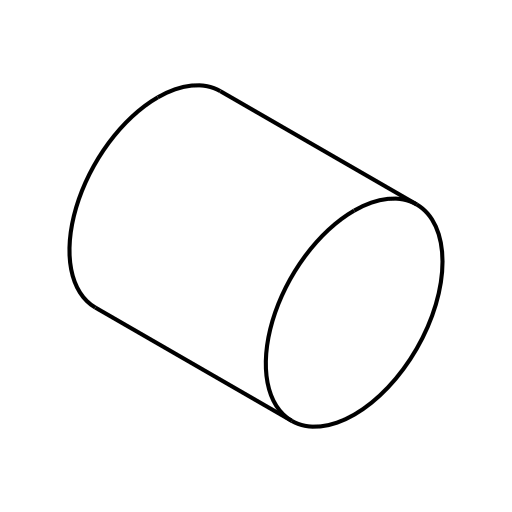
\includegraphics[width=\linewidth]{cylinder.png}
    \end{minipage}
    \hfill
    \begin{minipage}[]{0.5\textwidth}
        \centering
        \footnotesize
        \begin{verbatim}
{
  "sequence": [
    {
      "type": "Sketch",
      "entity": "sketch1_id"
    },
    {
      "type": "ExtrudeFeature",
      "entity": "extrude1_id"
    }
  ],
  "entities": {
    "sketch1_id": {
      "profiles": {
        "profile1_id": {
          "loops": [
            {
              "is_outer": true,
              "profile_curves": [
                {
                  "curve": "curve1_id",
                  "center_point": {
                    "x": 0.0,
                    "y": -50.0,
                    "z": 0.0
                  },
                  "radius": 45.0,
                  "normal": {
                    "x": 0.0,
                    "y": 1.0,
                    "z": 0.0
                  },
                  "type": "Circle3D"
                }
              ]
            }
          ]
        }
      },
      ...
    },
    "extrude1_id": {
      "reference_profiles": [
        {
          "parent": "sketch1_id",
          "id": "profile1_id"
        }
      ],
      "extent_one": {
        "distance": {
          "value": 100.0
        },
        ...
      }
    }
  }
}
\end{verbatim}
    \end{minipage}
    \caption{Представление цилиндра в формате CADAxt.}
\end{figure}

\newpage

Под ключом \texttt{sequence} идёт описание последовательности команд,
где \texttt{type}~--- тип операции, а \texttt{entity}~--- уникальный \texttt{id} операции.
Далее, под ключом \texttt{entities} хранится параметрическое описание каждой команды по соответствующему \texttt{id}.
Некоторые параметры здесь специально опущены, так как они не потребуются в~дальнейшем тексте.

Для понимания строения CAD-объекта обсудим параметры \texttt{Sketch}.
Каждый скетч состоит из \textit{loops} (замкнутых кривых) и \textit{profiles}.
Кривые (\texttt{curve}) бывают трёх типов: \texttt{Arc} (дуга), \texttt{Circle} (окружность) и \texttt{Line} (линия).
Безусловно, в реальном CAD-пакете есть и другие типы кривых (например, B-сплайны),
но в рамках данной работы мы ограничимся указанными тремя.
Набор \textit{Loop}, по которым можно однозначно определить ориентацию, формирует \textit{Profile}.
Валидный профиль всегда состоит из внешнего \textit{Loop} и внутренних непересекающихся,
причём внутренние задают отверстия во внешнем.

\begin{figure}[h!]
    \centering
    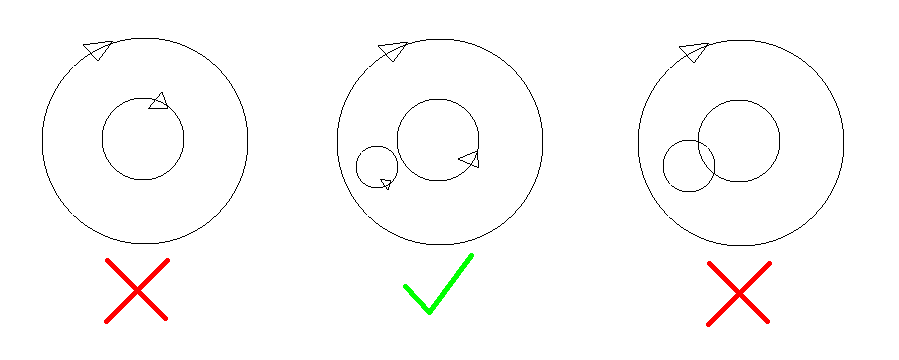
\includegraphics[width=0.7\textwidth]{sketches.png}
    \caption{Пример валидных и невалидных скетчей.}
    \label{fig:sketches}
\end{figure}

Координаты, описывающие скетч, заданы в трёхмерном пространстве относительно стандартной системы отсчёта.
Однако, по сути, скетч~--- это 2D-операция, задаваемая на плоскости.
При реализации \textit{profile} может быть вычислена плоскость, относительно которой рисуется скетч,
что даёт возможность отказаться от третьей координаты и задавать скетч параметрами плоскости и координатами в~этой плоскости.
В формате CADAxt для операции \texttt{Sketch} хранится параметр \texttt{transform}, указывающий плоскость,
относительно которой рисуется скетч.

Теперь рассмотрим параметры экструдирования:
\begin{enumerate}
    \item \texttt{profiles}~--- список профилей, к которым применяется экструд.
          Он однозначно задаётся путём указания \texttt{id} скетча и \texttt{id} нужного профиля.
    \item \texttt{extent\_one}~--- величина, на которую выдавливается скетч по направлению его нормали.
          Направление может меняться при наличии дополнительных параметров, специально опущенных здесь.
\end{enumerate}

Таким образом, описанный формат даёт полноценное описание \textit{constructive sequence}
относительно операций \texttt{Sketch} и \texttt{Extrude}. Не рекомендуется использовать его напрямую для генерации,
так как размер подобного файла может достигать нескольких тысяч символов.
Однако он легко транслируется в любые иные форматы, что является существенным преимуществом при тестировании различных представлений.

\subsection{CADQuery и CADScript.}

После создания унифицированного формата необходимо решить три основные задачи:
\begin{enumerate}
    \item Определить, какие форматы представления CAD будут сравниваться.
    \item Определить, на каких данных будет происходить обучение.
    \item Выбрать архитектуру модели, подходящую для решения поставленной задачи.
\end{enumerate}

Отвечая на первый вопрос, на ум сразу приходят форматы \texttt{CADQuery} и \texttt{PythonOCC}.
\texttt{PythonOCC}~--- это низкоуровневый способ создания CAD-объектов, основанный на технологиях OpenCascade.
Формат \texttt{CADQuery} представляет собой надстройку над \texttt{PythonOCC} и обеспечивает более удобный
способ записи. По сути, \texttt{CADQuery} является набором макросов над \texttt{PythonOCC}, благодаря чему
код одной и той же топологии получается более компактным именно в \texttt{CADQuery}. Тем не менее
сравнивать эти два формата на равных основаниях некорректно, поэтому необходимо подобрать ещё один формат,
который, с одной стороны, будет иметь более лаконичное представление, а с другой --- позволит сопоставить его
с \texttt{CADQuery}.

В литературе был предложен формат \texttt{OpenECAD}~\cite{yuan24_openecad}, в котором чётко описаны правила
оформления и представления скетчей. Основные моменты, выделяемые в \texttt{OpenECAD}, следующие:
\begin{enumerate}
    \item Моделирование в CAD обычно сводится к последовательности операций, приводящих к созданию твердотельных форм.
          В \texttt{OpenECAD} эти операции оформляются в виде структурированных команд.
    \item Скетчи в \texttt{OpenECAD} задаются на плоскости и определяются с помощью примитивов:
          линий, дуг и окружностей, а также их параметров.
    \item Для получения трёхмерных объектов в \texttt{OpenECAD} используется исключительно операция
          «скетч-экструзия», когда 2D-скетч преобразуется в 3D-форму за счёт протяжки.
    \item В \texttt{OpenECAD} применяются читаемые обозначения операций, что облегчает понимание
          и использование кода.
\end{enumerate}

\texttt{CADQuery}~— это большая библиотека с богатым набором функций и селекторов. Однако у неё есть
один недостаток: нет встроенного селектора, позволяющего выбирать рёбра, образованные конкретной
операцией (например, экструзией). Такой селектор важен при генерации последовательности действий:
если инженер в процессе проектирования видит текущее состояние 3D-модели и выбирает конкретное
ребро, плоскость или точку, то генератору необходимо отслеживать, какие элементы были созданы на предыдущих шагах.

В \texttt{OpenECAD} формат описания CAD-объектов более избыточен, однако он удобен для реализации
подобных селекторов. Из-за этой гибкости код в \texttt{OpenECAD} может получаться длиннее, чем в
\texttt{CADQuery}.

На основе подхода из \texttt{OpenECAD} был разработан формат \texttt{CADScript}. Его главное отличие
заключается в том, что он поддерживает дополнительные операции, не рассматриваемые в данной работе,
а также предусматривает квантизацию.

Примеры кода для двух представлений показаны на рисунке~\ref{fig:cadformats}.

\begin{figure}[h!]
    \centering
    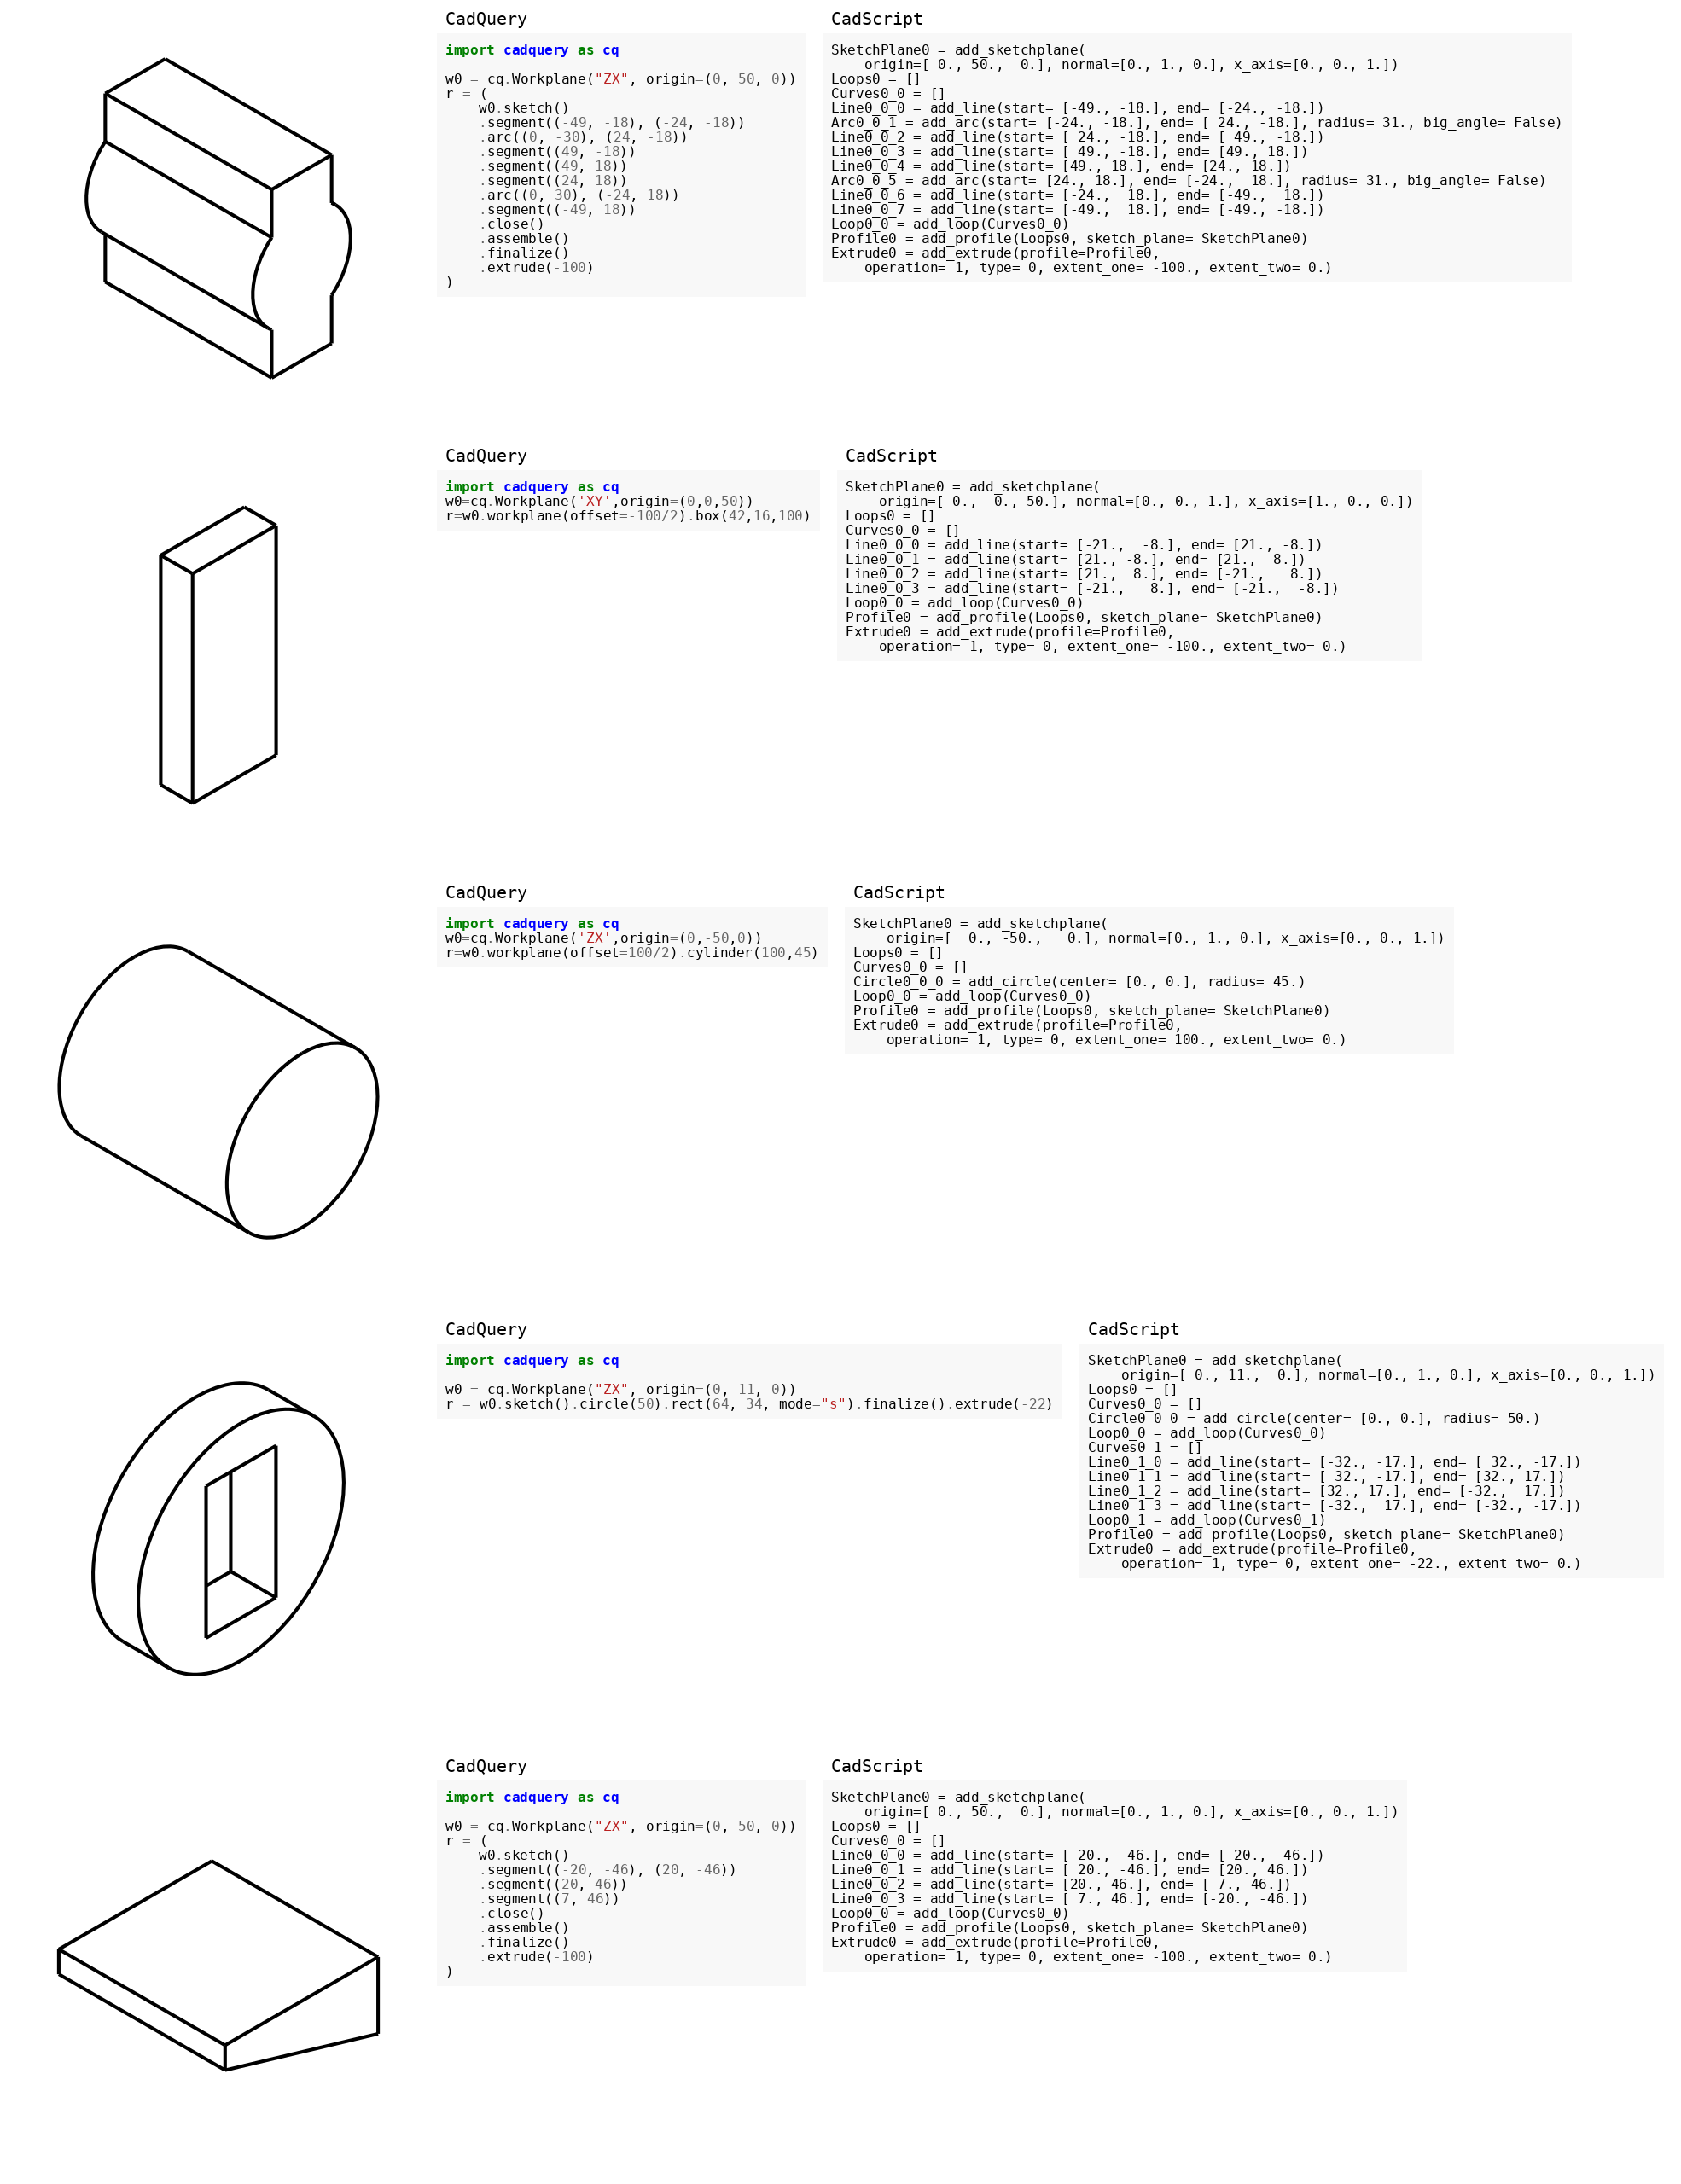
\includegraphics[width=1\textwidth]{stacked_result.png}
    \caption{Примеры представлений \texttt{CADQuery} и \texttt{CADScript}.}
    \label{fig:cadformats}
\end{figure}

\paragraph{Использование CADRecode и связка с CADAxt.}
Для решения второго и третьего вопросов в работе было выбрано решение
\texttt{CADRecode}. Его автор в своей статье разработал генератор синтетических
данных, которые показали лучшие результаты на бенчмарках DeepCAD и Fusion360.
Архитектура модели в \texttt{CADRecode} достаточно проста и быстро обучается,
не требуя больших вычислительных ресурсов.

В рамках настоящей работы было принято решение встроить в генератор
\texttt{CADRecode} конвейер перевода в универсальный формат \texttt{CADAxt}, из
которого затем реализован трансфер в \texttt{CADQuery} и
\texttt{CADScript}. После этого модель обучалась на одних и тех же облаках точек,
но с различными кодовыми представлениями.

Генератор одного миллиона синтетических данных работал в течение 7,5 часов на 8 H100
используя 96 CPU. То есть скорость генерации одного семпла составляет 0.4/sec на одном ядре

\subsection{Подход CAD-Recode.}

\begin{figure}[h!]
    \centering
    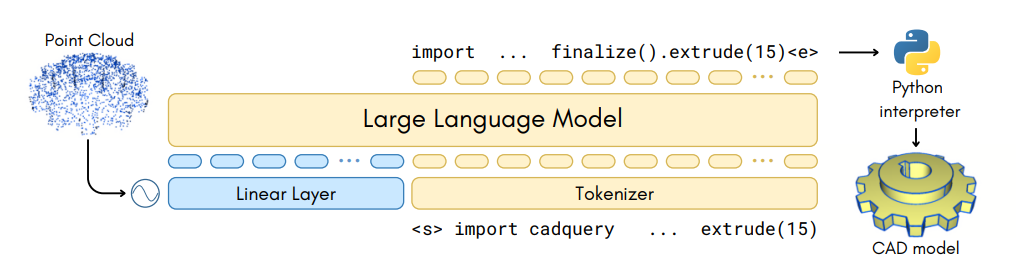
\includegraphics[width=1\textwidth]{cadrecode_arc.png}
    \caption{Архитектура CAD-Recode}
    \label{fig:cadrecode_arc}
\end{figure}

\texttt{CAD-Recode} опирается на предварительно обученных специалистов и их опыт
работы с Python-кодом, дополняя их возможностями по обработке облаков точек, а
также знаниями, специфичными для CAD-кода на Python. Как показано на рис.~4 в
оригинальной статье, архитектура \texttt{CAD-Recode} состоит из двух частей:
(1)~проектора облака точек, преобразующего 3D-облако точек в обучаемые токены, и
(2)~предварительно обученного авторегрессионного CAD-декодера на базе LLM.

\textbf{Модуль проекции облака точек.} В \texttt{CAD-Recode} представлен лёгкий
модуль проекции~$\Psi_P$, который напрямую отображает плотное облако точек
$P \in \mathbb{R}^{n \times d_p}$ (где $d_p = 3$ соответствует размерности
координат) в последовательность из $n_p$ токенов $Q_p = [q^1_p, \dots, q^{n_p}_p]
    \in \mathbb{R}^{n_p \times d_q}$, где $d_q$~--- размерность встраивания. Модуль
проекции, обучаемый совместно с модулем CAD-код-декодера, состоит из трёх простых
компонентов: (1)~алгоритма выбора самых удалённых точек для уменьшения входного
облака точек до $n_p$; (2)~позиционного кодирования координат методом Фурье;
(3)~линейного слоя, проецирующего закодированные координаты в $Q_p$.

\textbf{LLM в качестве CAD-декодера.} В качестве CAD-декодера кода, обозначаемого
$\Psi_{\text{LLM}}$, выступает предварительно обученный LLM-специалист,
приспособленный к задаче генерации кода CAD. В качестве базы берётся модель
\texttt{Qwen2-7b}. На вход этому декодеру подаются токены $Q_p$ от проектора облака точек,
дополненные кодовыми токенами $Q_t \in \mathbb{R}^{n_t \times d_q}$,
полученными после токенизации входного кода. Полная
входная последовательность обозначается $[Q_p; Q_t] \in
    \mathbb{R}^{(n_p + n_t) \times d_q}$. Модель предсказывает следующую часть
кодовой последовательности CAD, сопоставляя каждый предсказанный токен с
символом из словаря~$\Sigma$ (буквенно-цифровые символы и операторы). Таким
образом, \texttt{CAD-Recode} перенастраивает возможности моделирования LLM для
задачи преобразования облаков точек в исполняемый CAD-код.

\subsection{Процесс обучения.}
Стратегия обучения состоит из одного этапа. Модель работает с токенами запроса
размерности $d_q = 1536$ и обрабатывает изначальные облака точек в момент,
когда их количество уменьшено до $n_p = 256$. К~координатам входных точек
добавляется гауссовский шум со средним ноль и стандартным отклонением 0.01 с
вероятностью 0.5. Модель обучают на~процедурно сгенерированных CAD-кодах, где
доступен набор функций CAD и методов проектирования, включённых в~алгоритм
генерации. Цель обучения~--- минимизация ошибки \emph{Negative Log Likelihood}
(NLL). При этом последовательность CAD-кода ограничивается специальными
маркерами \texttt{<s>} и \texttt{<e>}. Модуль проекции облака точек изучает
геометрические объекты \emph{с нуля}, а предварительно обученный декодер
донастраивается под задачу генерации CAD-кода.

\subsection{Метрики и эксперимент.}
Для оценки качества генерируемого CAD-кода в последовательностях создания
эскизов использовались три основных метрики:
\begin{enumerate}
    \item \emph{Chamfer Distance} (CD).
    \item \emph{Intersection over Union} (IoU).
    \item \emph{Invalid Rate} (IR).
\end{enumerate}

Результаты представлены как в виде среднего значения по выборке.
Значение CD рассчитывалось с использованием 8192 точек и умножалось на \(10^3\).
Показатель IoU вычислялся на основе объединённых сеток CAD-моделей и выражался
в процентах. IR указывает процент сгенерированных последовательностей,
которые оказались некорректными для построения модели CAD.

Ниже приведены используемые формулы для перечисленных метрик.

\paragraph{Chamfer Distance (CD).}
Пусть \( X \) и \( Y \) --- два множества точек, взятых равномерной выборкой
с поверхностей двух 3D-моделей. Тогда метрика Chamfer Distance определяется как:
\[
    \mathrm{CD}(X, Y) \;=\; \frac{1}{|X|}\sum_{x\in X}\min_{y\in Y}\|x - y\|^2
    \;+\;
    \frac{1}{|Y|}\sum_{y\in Y}\min_{x\in X}\|y - x\|^2.
\]
В коде это реализуется путём выборки фиксированного числа точек \(n\) (в примере \(n = 8192\))
с последующим вычислением среднеквадратичных расстояний от каждой точки одной модели
до ближайшей точки другой модели.

\paragraph{Intersection over Union (IoU).}
Пусть \( A \) и \( B \) --- объёмы (или сетки) двух 3D-моделей в пространстве.
Тогда метрика IoU определяется как отношение объёма пересечения к объёму объединения:
\[
    \mathrm{IoU}(A, B) \;=\; \frac{\mathrm{Vol}\bigl(A \cap B\bigr)}
    {\mathrm{Vol}\bigl(A \cup B\bigr)}.
\]
В коде это достигается путём разбиения сеток на отдельные части,
вычисления их пересечения и суммирования объёмов.

\paragraph{Invalid Rate (IR).}
Пусть имеется общее число сгенерированных последовательностей \(N\),
из которых \(M\) оказываются некорректными для построения 3D-модели.
Тогда метрика IR вычисляется следующим образом:
\[
    \mathrm{IR} \;=\; \frac{M}{N}.
\]
Она показывает долю сгенерированных решений, которые не удалось корректно
преобразовать в итоговую CAD-модель.

Обучение проводилось на различном количестве карт H100 и~при разных размерах
батча, поскольку длина кода в разных форматах отличается.

\begin{table}[h!]
    \centering
    \caption{Условия обучения}
    \begin{tabular}{|l|c|c|c|c|c|}
        \hline
        Format    & H100 & Batch size & Run time & Max code length & Epoch \\ \hline
        CADQuery  & 4    & 9          & 3d       & 800             & 10    \\ \hline
        CADScript & 6    & 6          & 3d17     & 2517            & 10    \\ \hline
    \end{tabular}
\end{table}

Эксперименты проводились на трёх тестовых наборах по 1000 моделей: DeepCAD,
Fusion360, CC3D и CAD-Recode. Облака точек для DeepCAD и Fusion360 получены путём выборки точек на сетках, а набор
CC3D содержит реальные 3D-сканы с шумом, сглаженными краями и отсутствующими деталями.
Ниже на рисунке \ref{fig:datasets1} \ref{fig:datasets2} представлены примеры семплов из каждого датасета

\newpage

\begin{figure}[h!]
    \centering
    % Первая картинка на всю ширину
    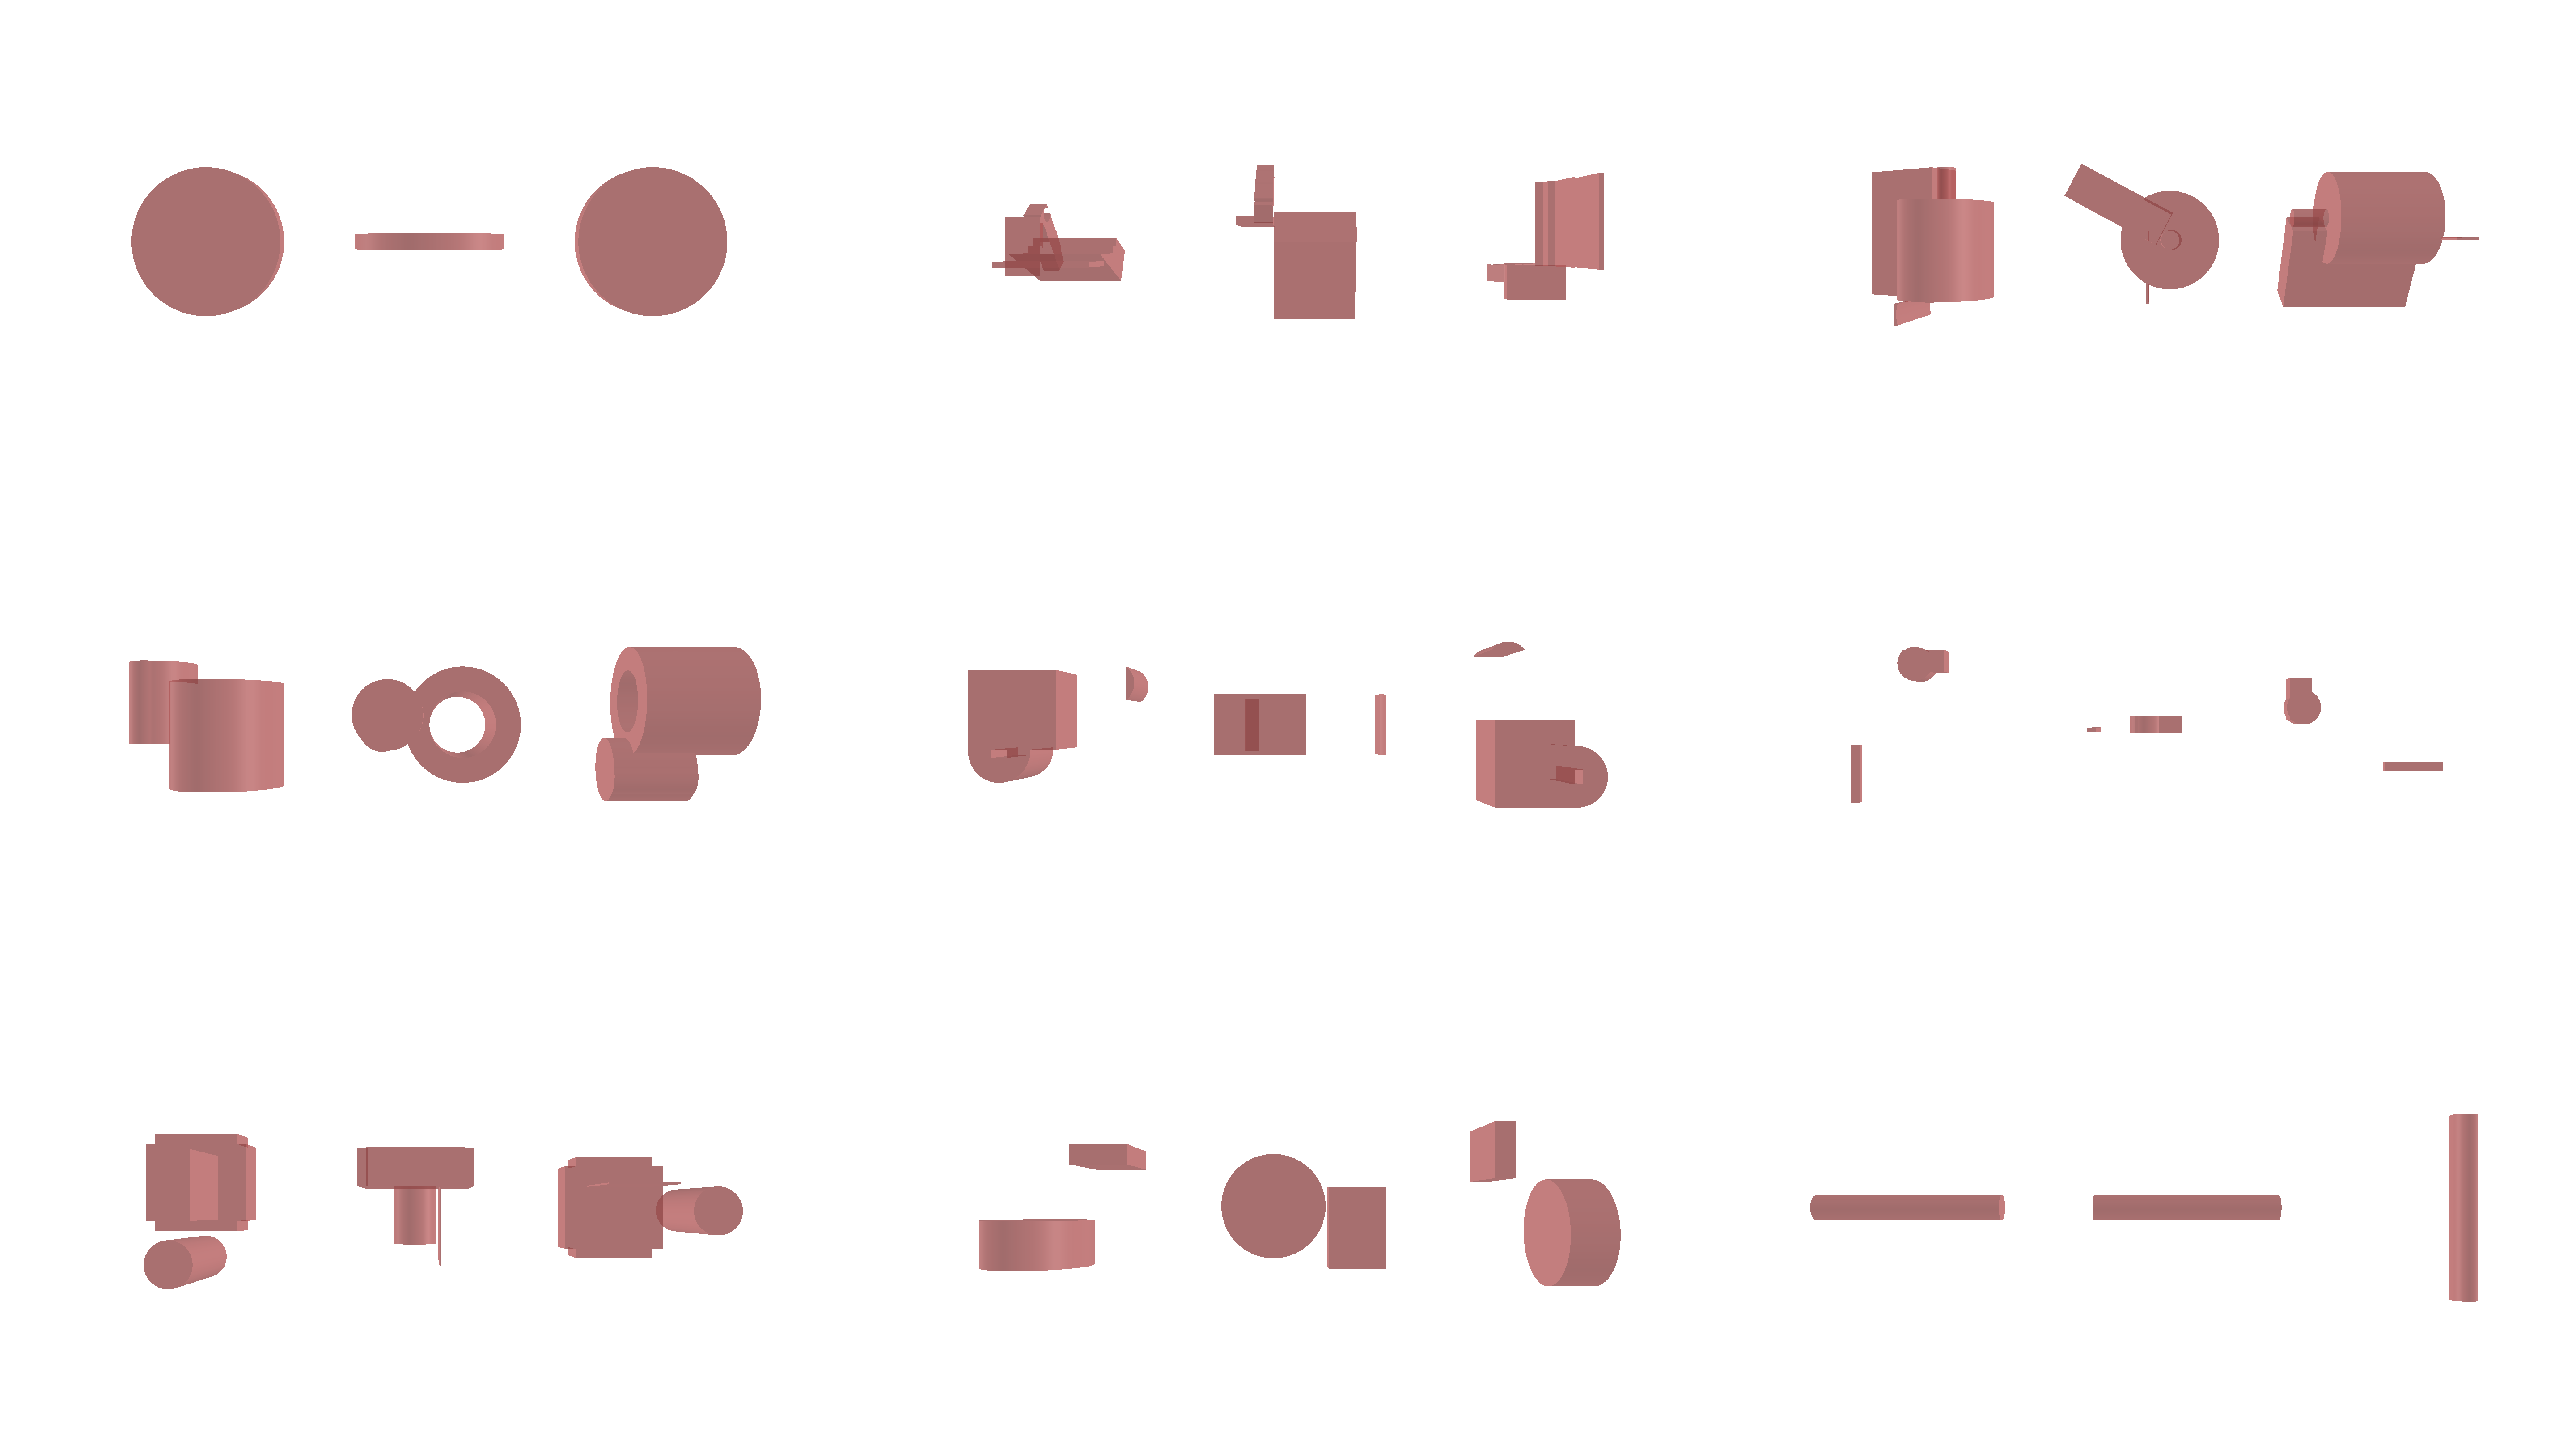
\includegraphics[width=\textwidth]{cadrecode_set.png}
    \caption{CAD-Recode}

    \vspace{1em} % небольшой отступ между картинками

    % Вторая картинка на всю ширину
    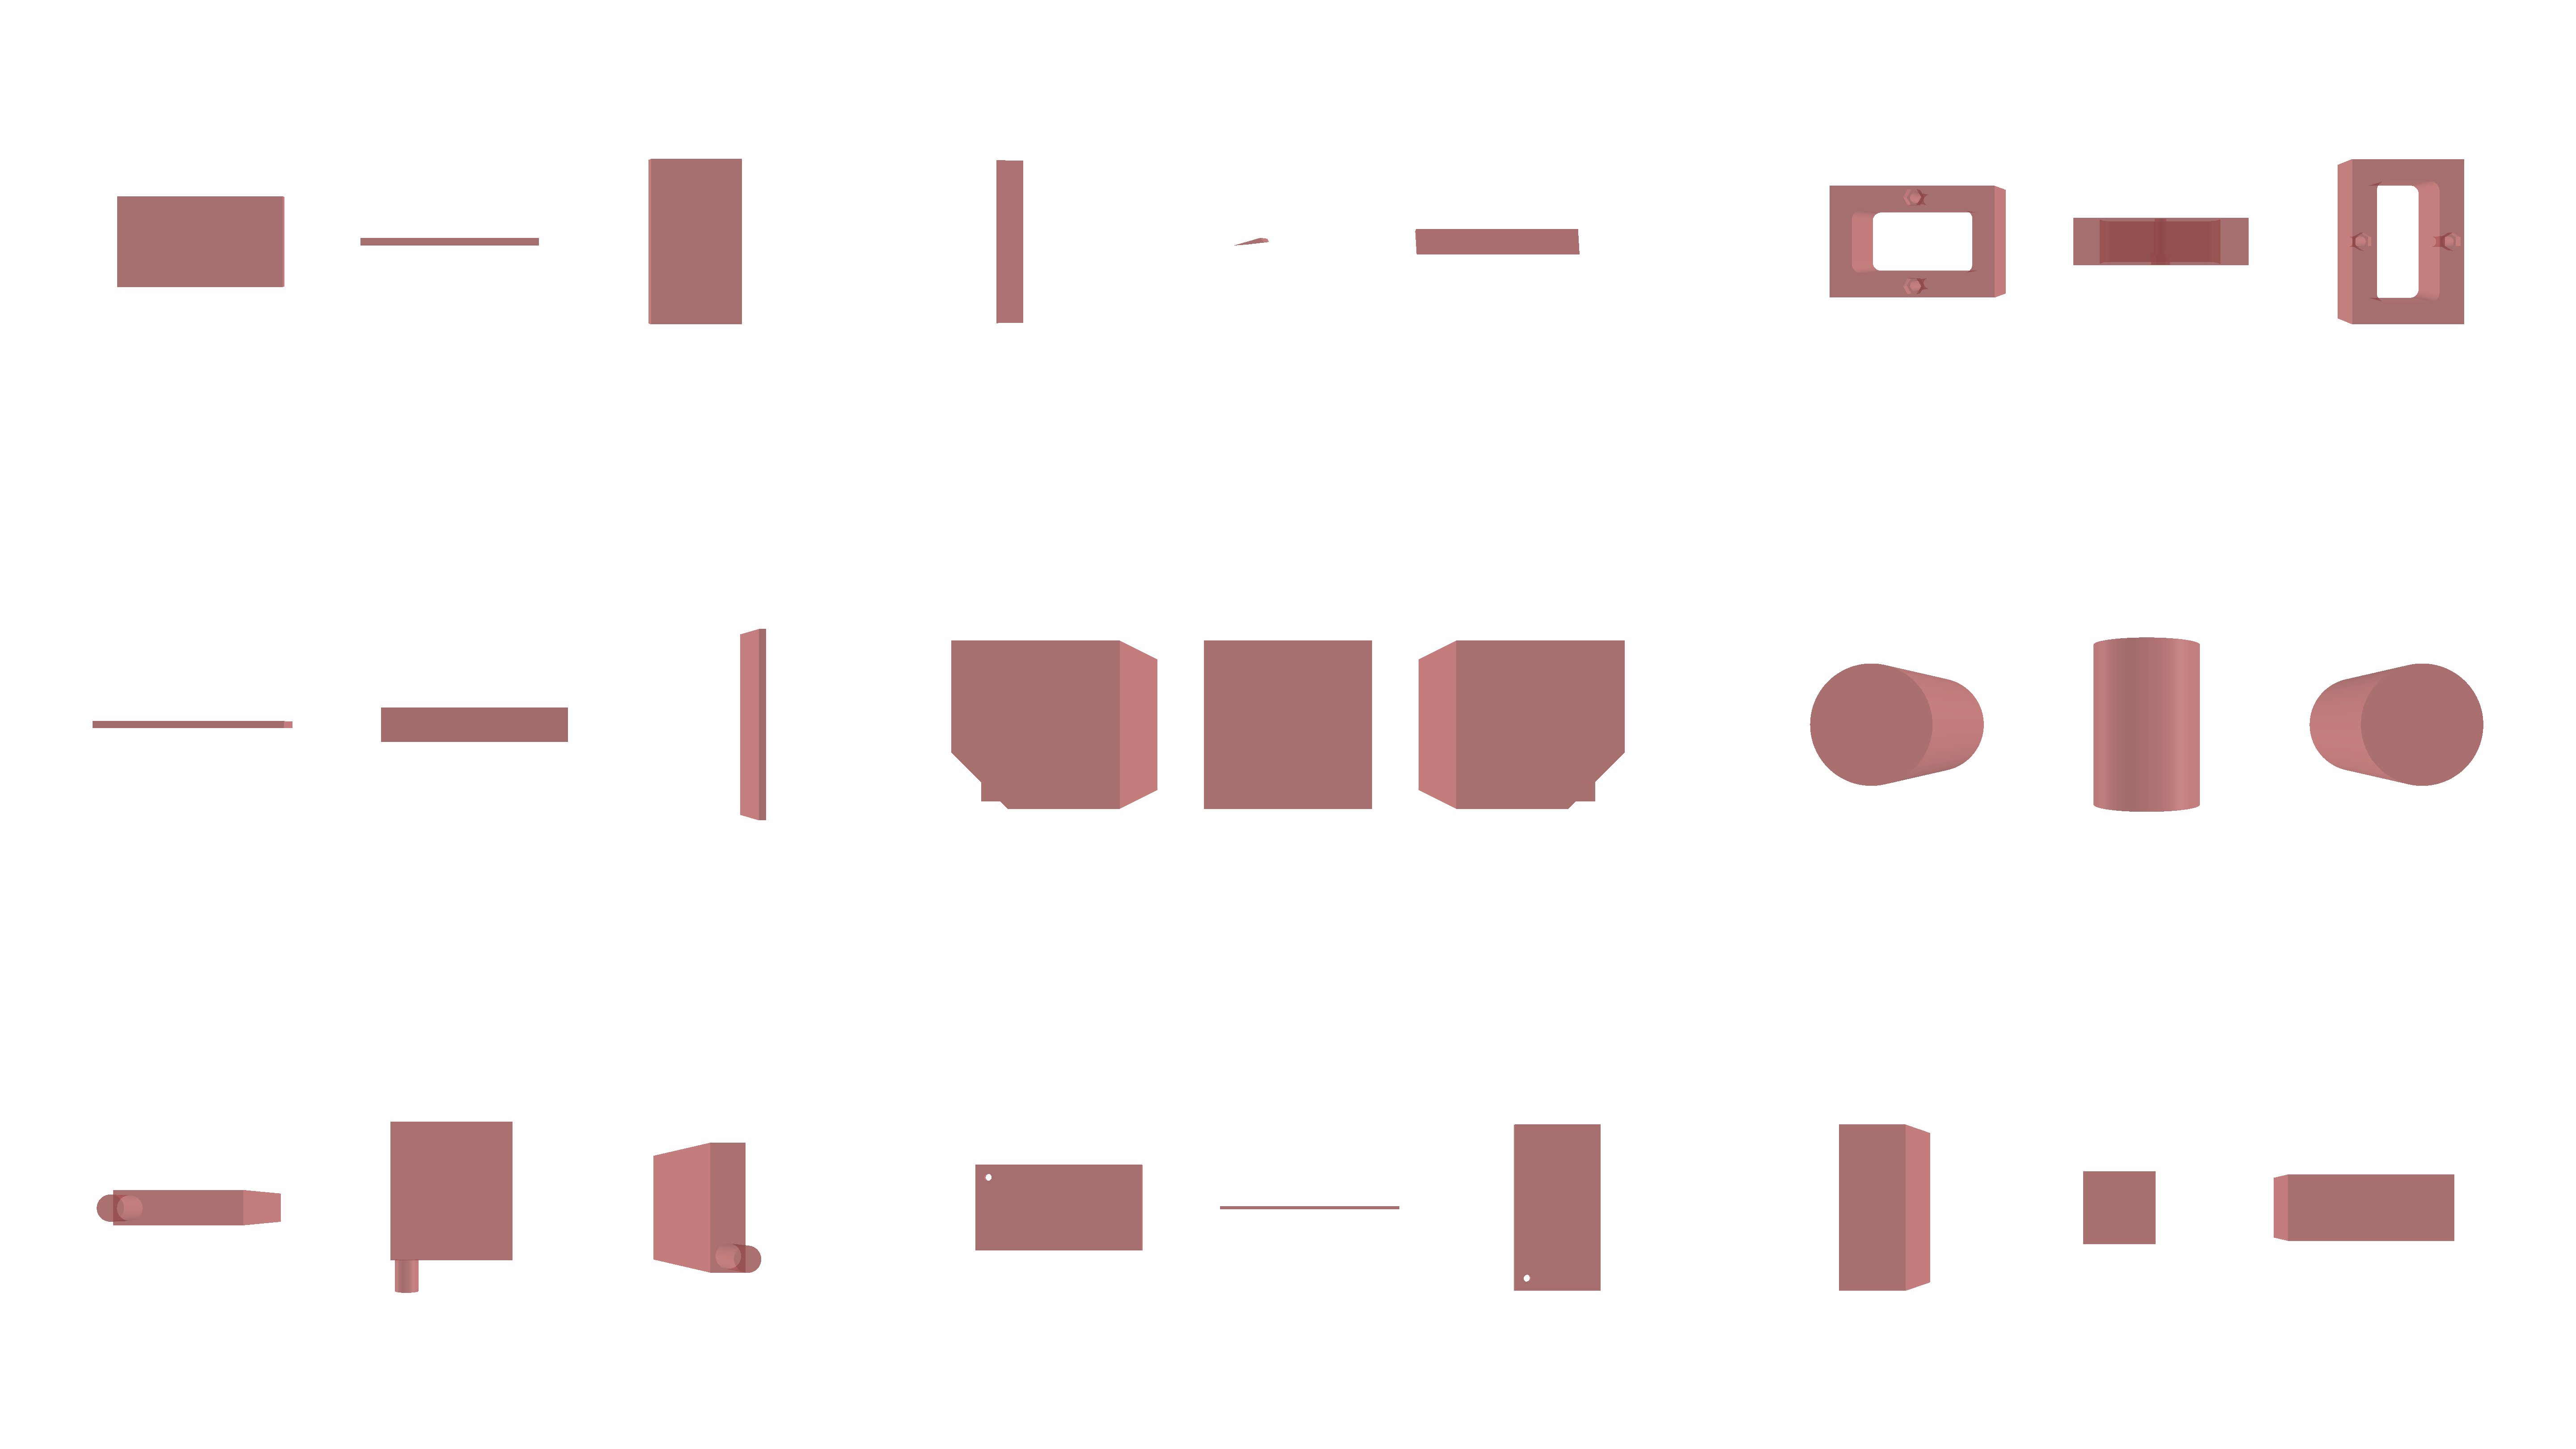
\includegraphics[width=\textwidth]{deepcad_set.png}
    \caption{DeepCAD}

    \caption{Примеры данных из валидационных наборов CAD-Recode и DeepCAD}
    \label{fig:datasets1}
\end{figure}

\newpage

\begin{figure}[h!]
    \centering
    % Первая картинка на всю ширину
    % Третья картинка на всю ширину
    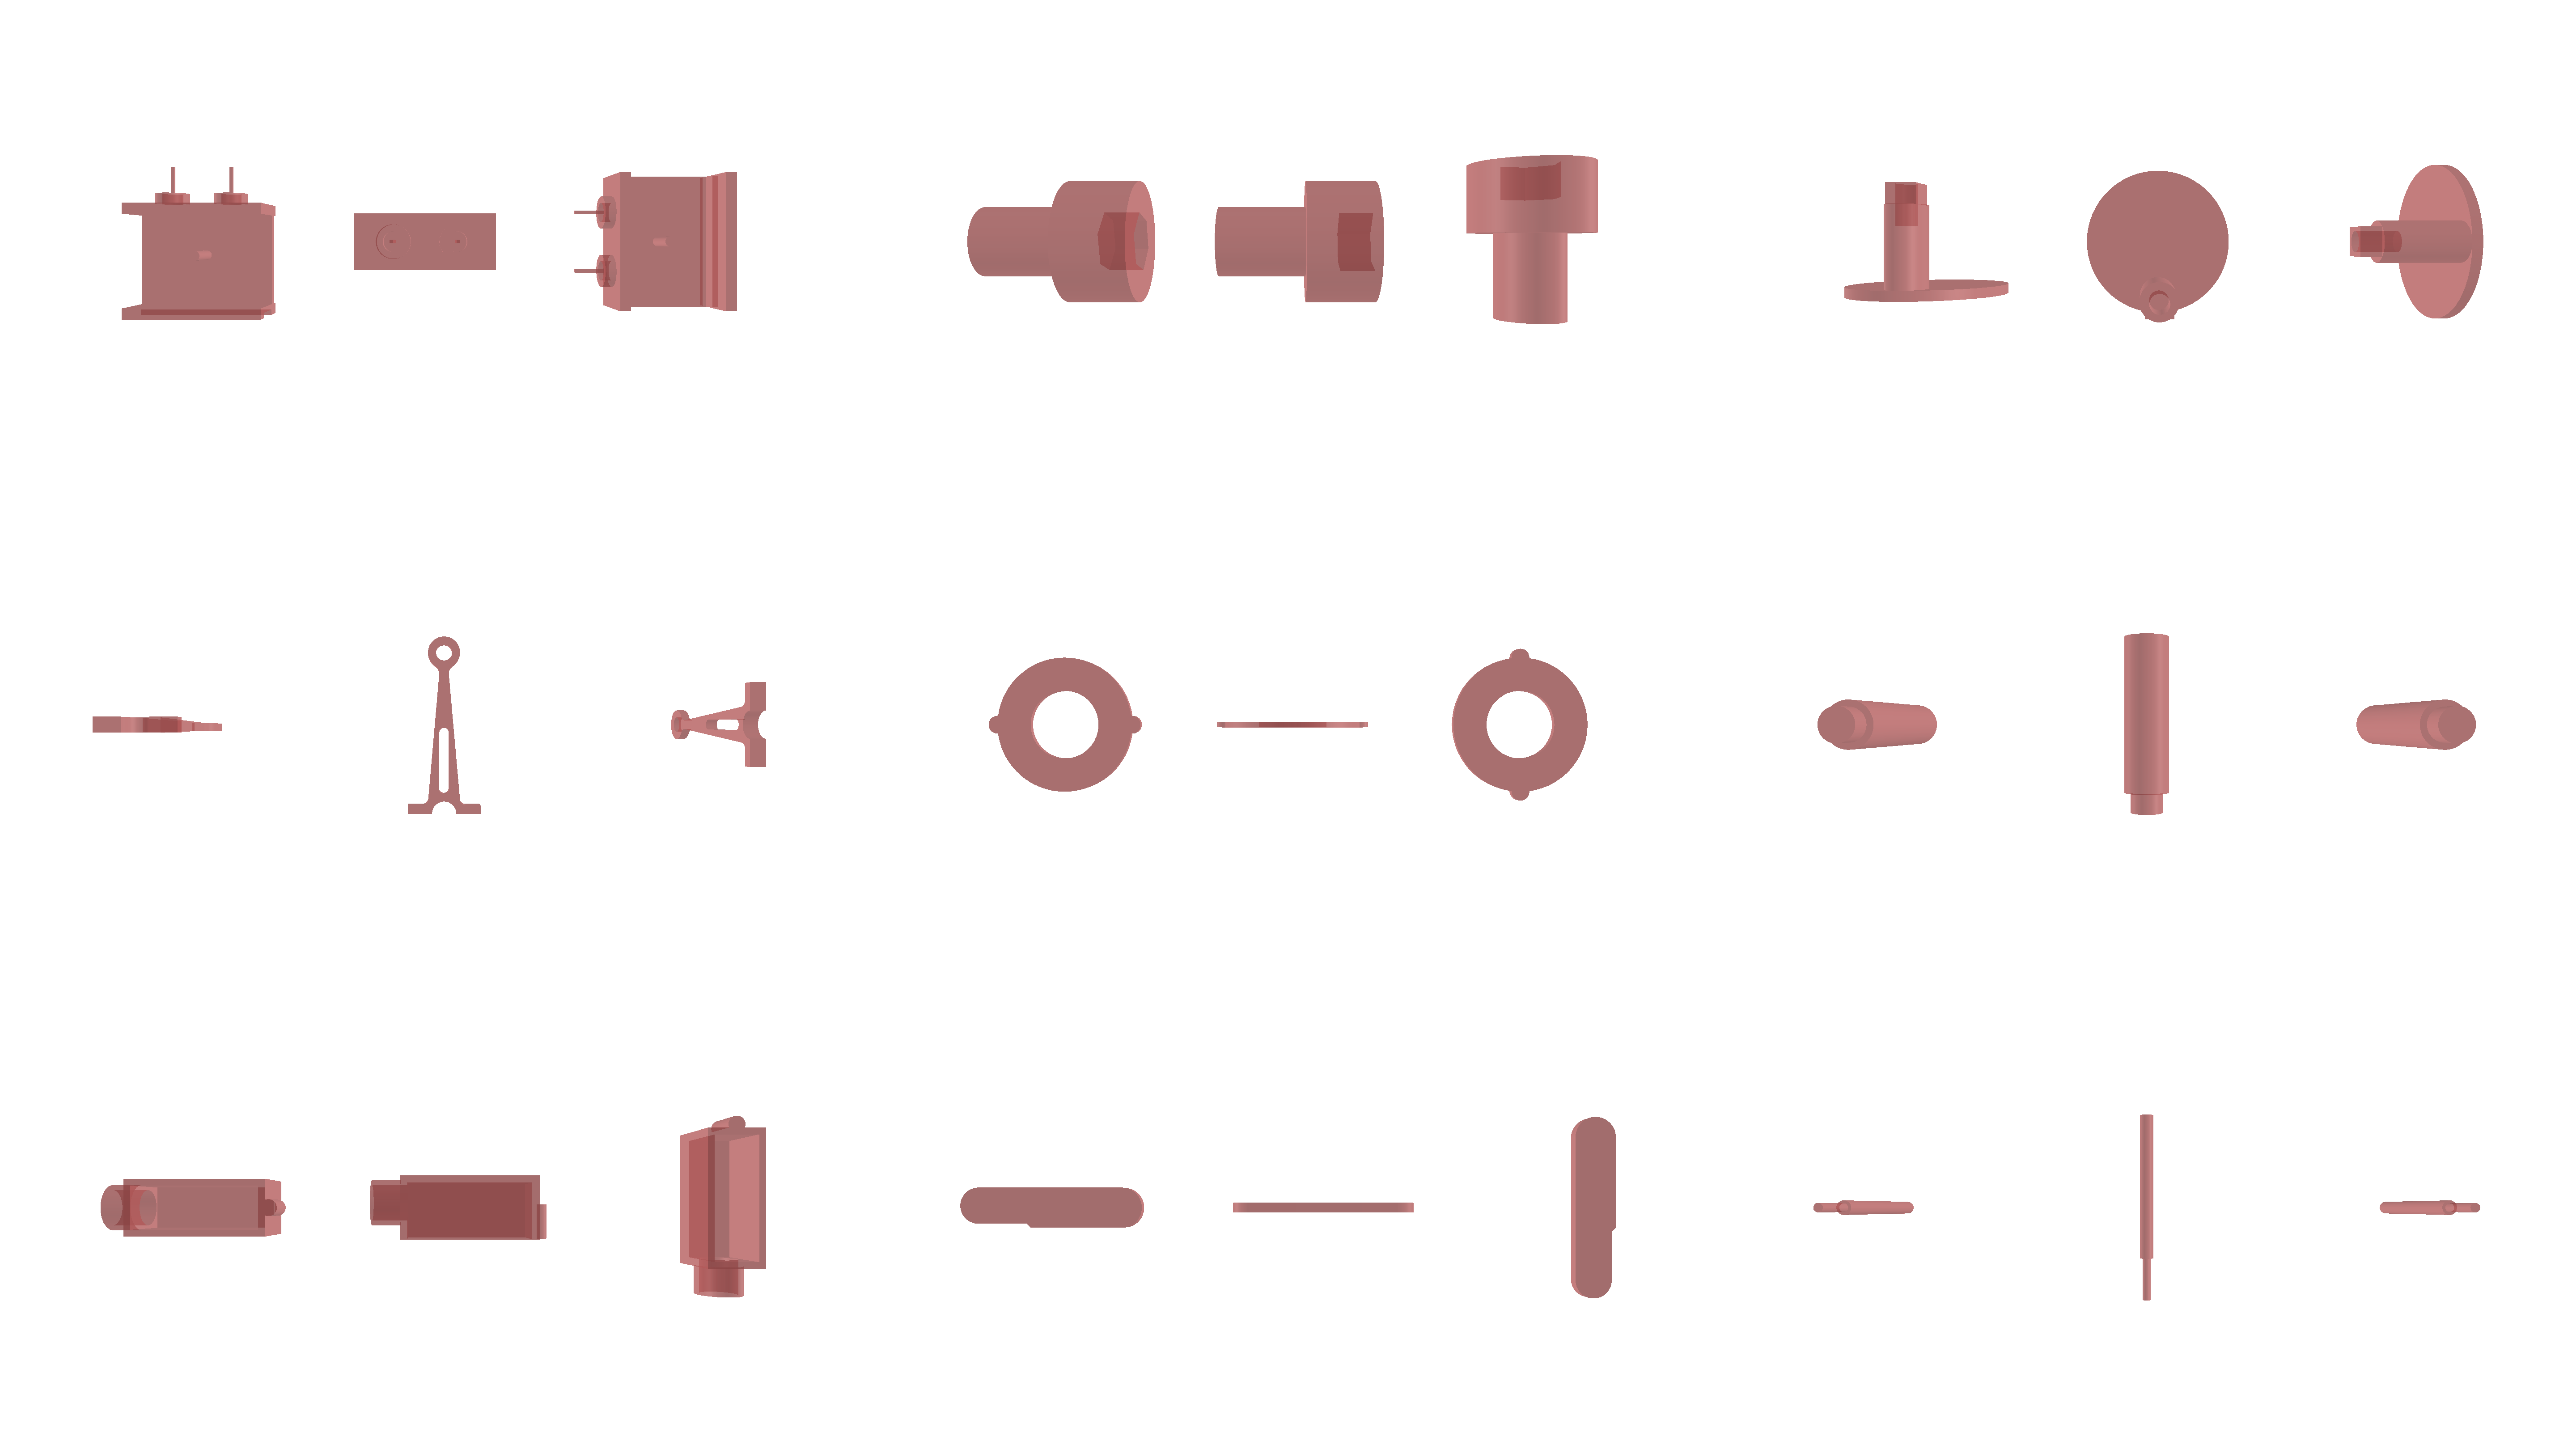
\includegraphics[width=\textwidth]{fusion360_set.png}
    \caption{Fusion360}

    \vspace{1em}

    % Четвёртая картинка на всю ширину
    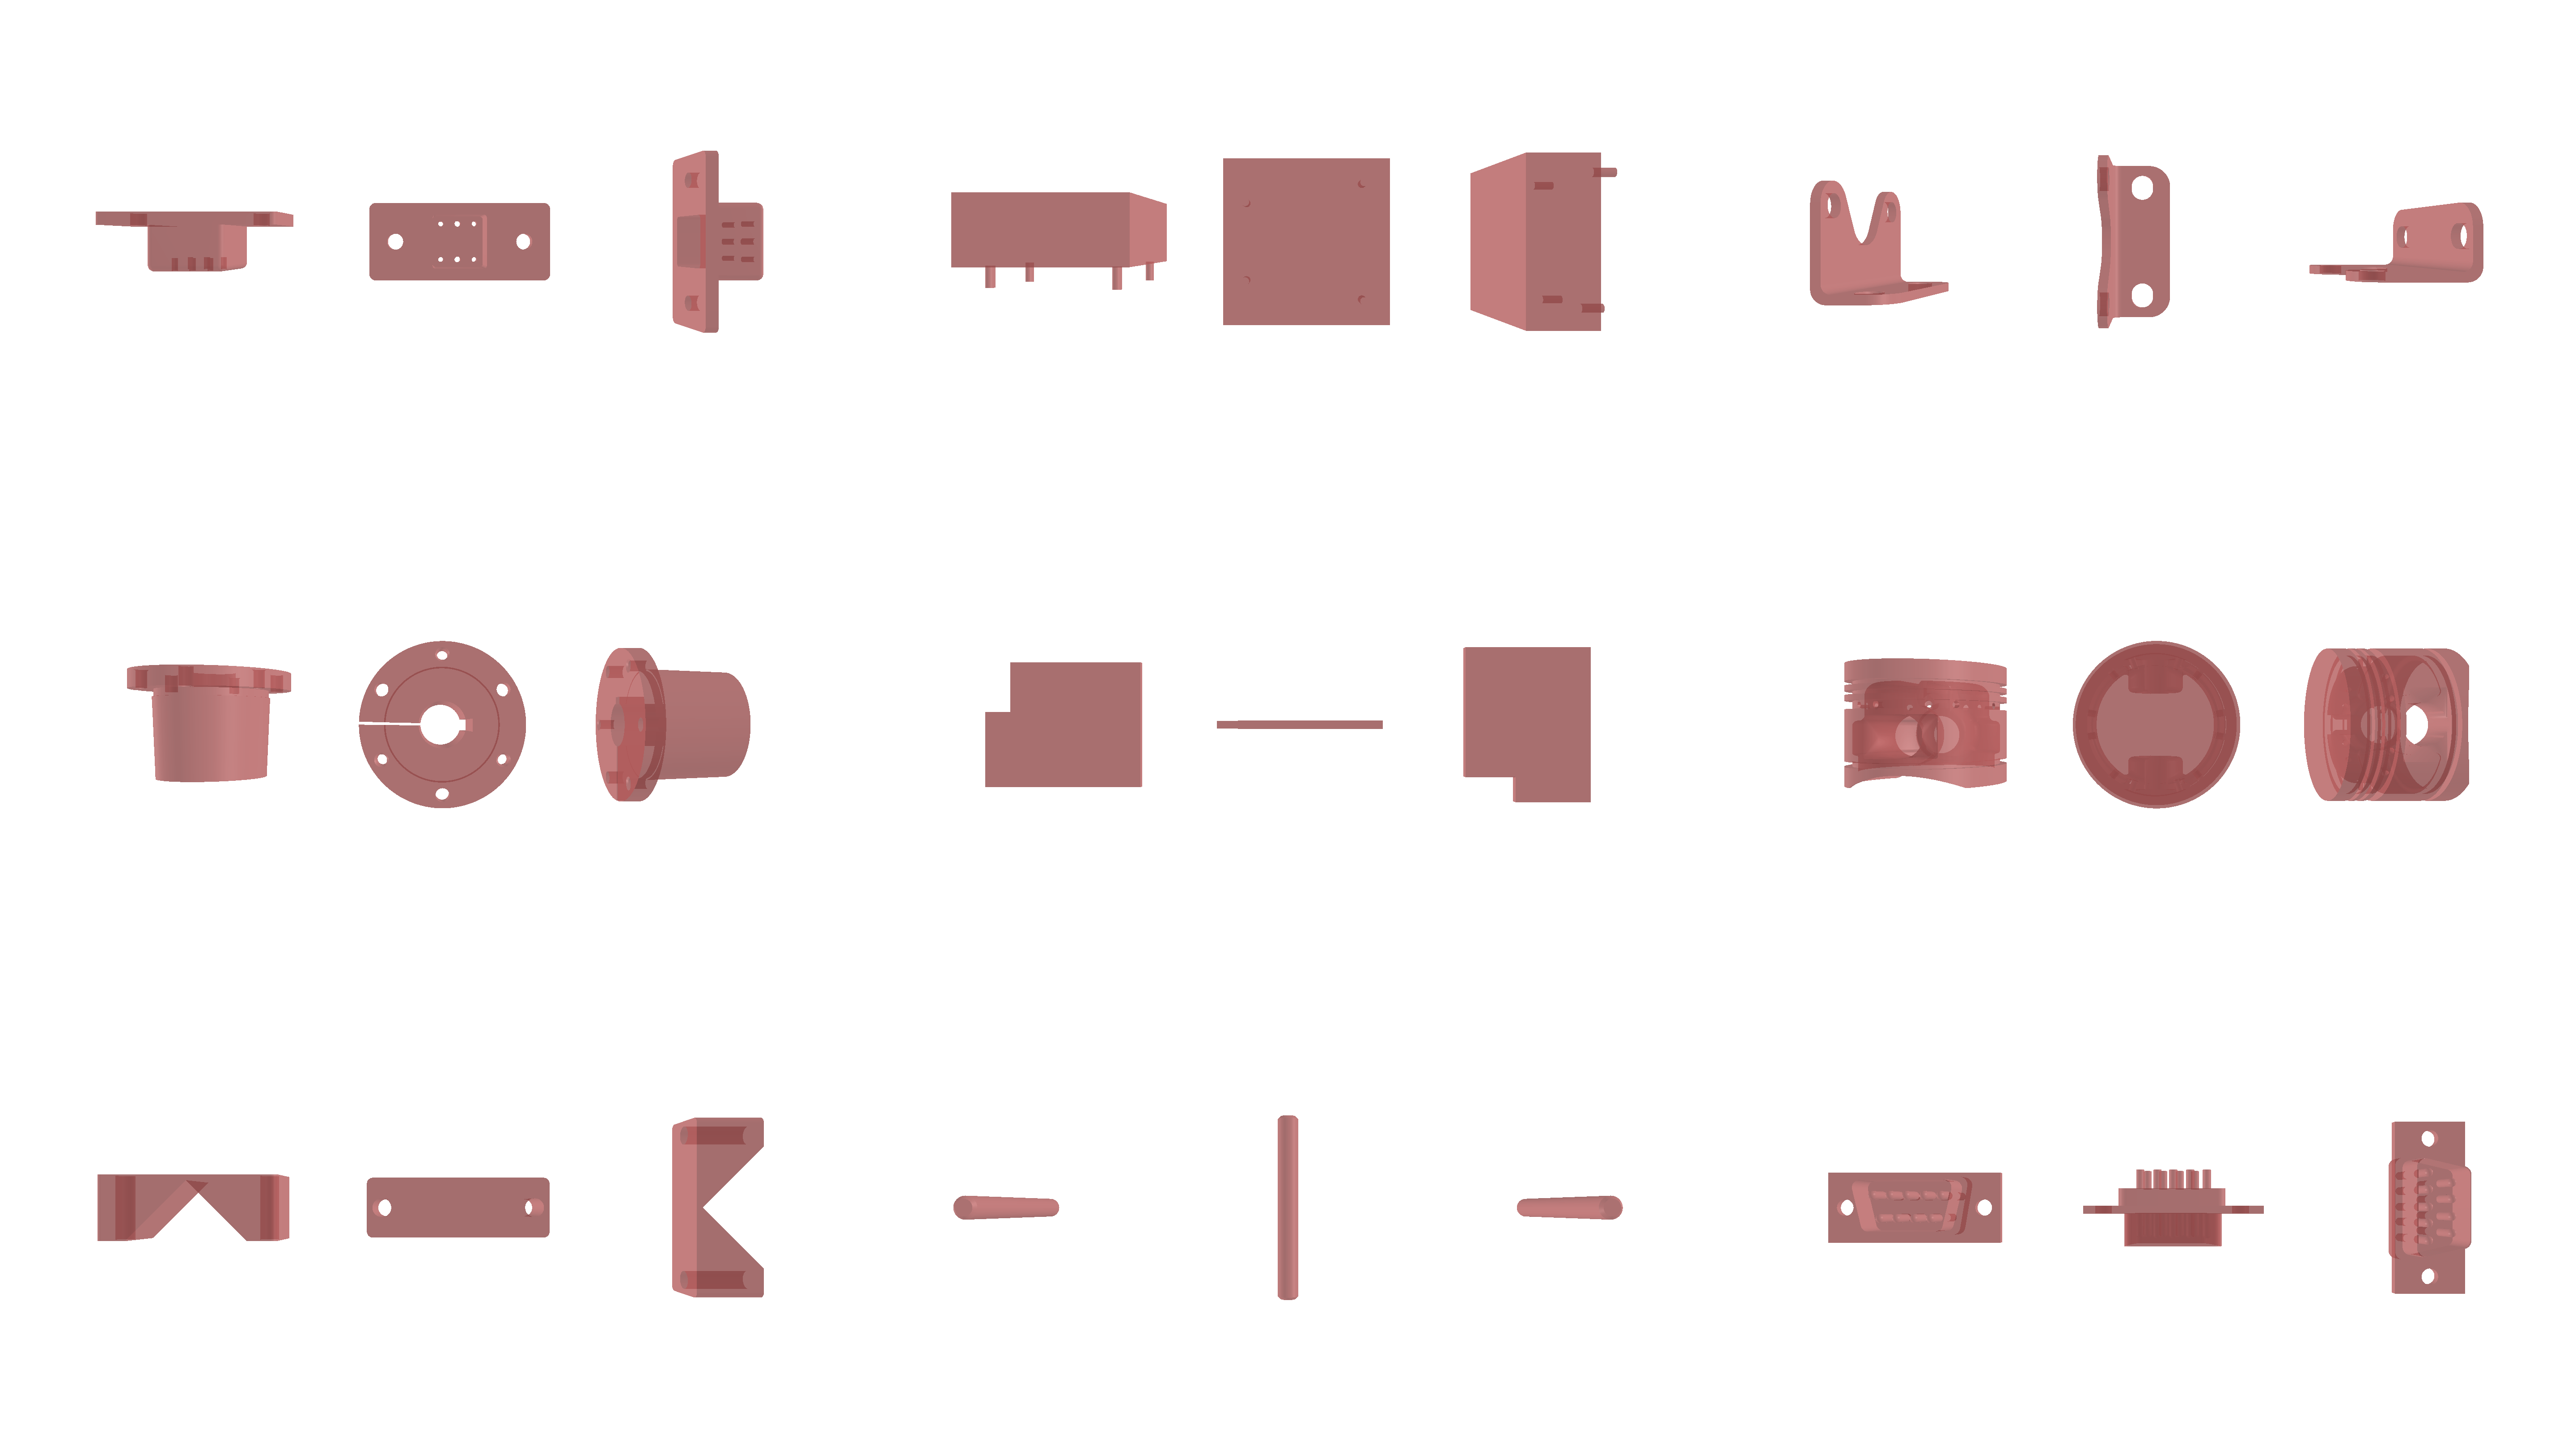
\includegraphics[width=\textwidth]{cc3d_set.png}
    \caption{CC3D}

    \caption{Примеры данных из валидационных наборов Fusion360 и CC3D}
    \label{fig:datasets2}
\end{figure}

\newpage

\subsection{Результаты и анализ.}

Я проведу анализ каждой эпохи на выше описанных датасетах, это позволит нам понять тренд обучения и проанализировать закономерности.

Сводные таблицы с метриками оказываются очень громоздкими и малоинформативными, поэтому анализ будет произведен на графиках.

\begin{figure}[h!]
    \centering
    \begin{subfigure}{0.45\linewidth}
        \centering
        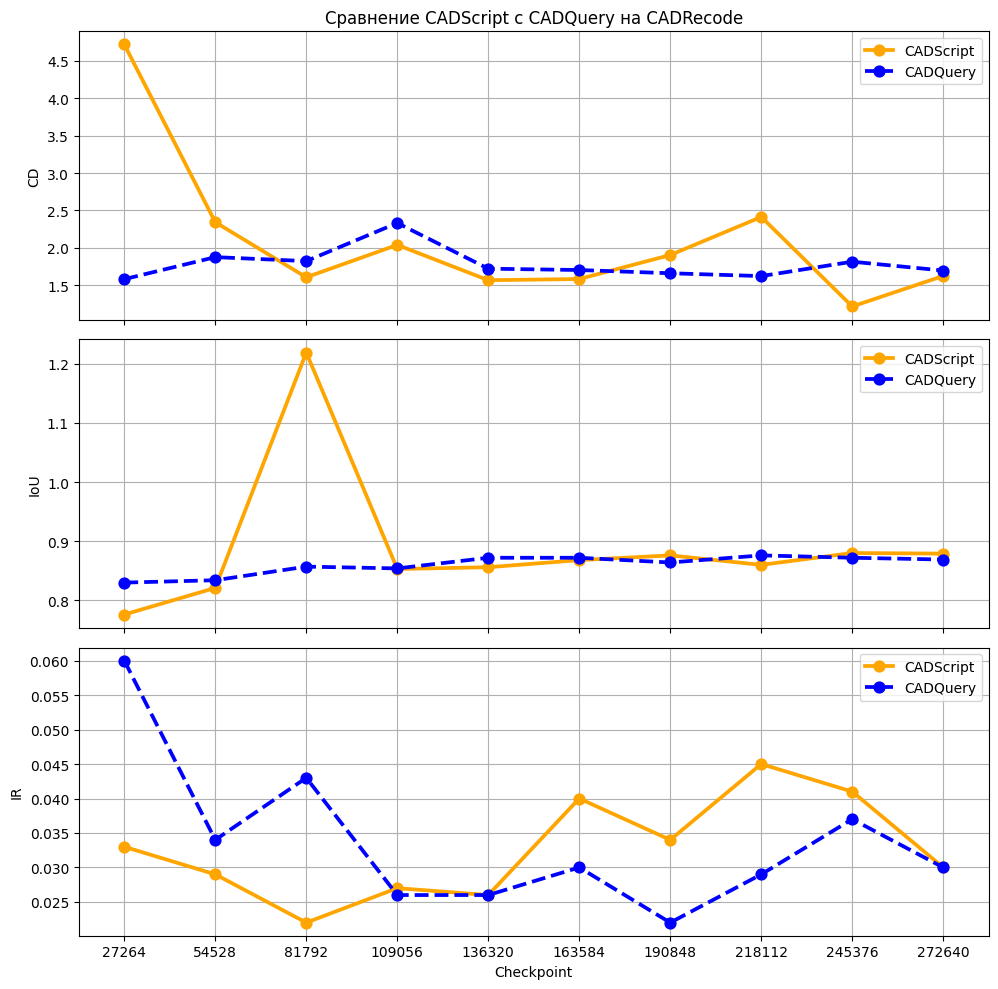
\includegraphics[width=\linewidth]{formats/formats_cadrecode.png}
        \caption{CAD-Recode}
    \end{subfigure}
    \hfill
    \begin{subfigure}{0.45\linewidth}
        \centering
        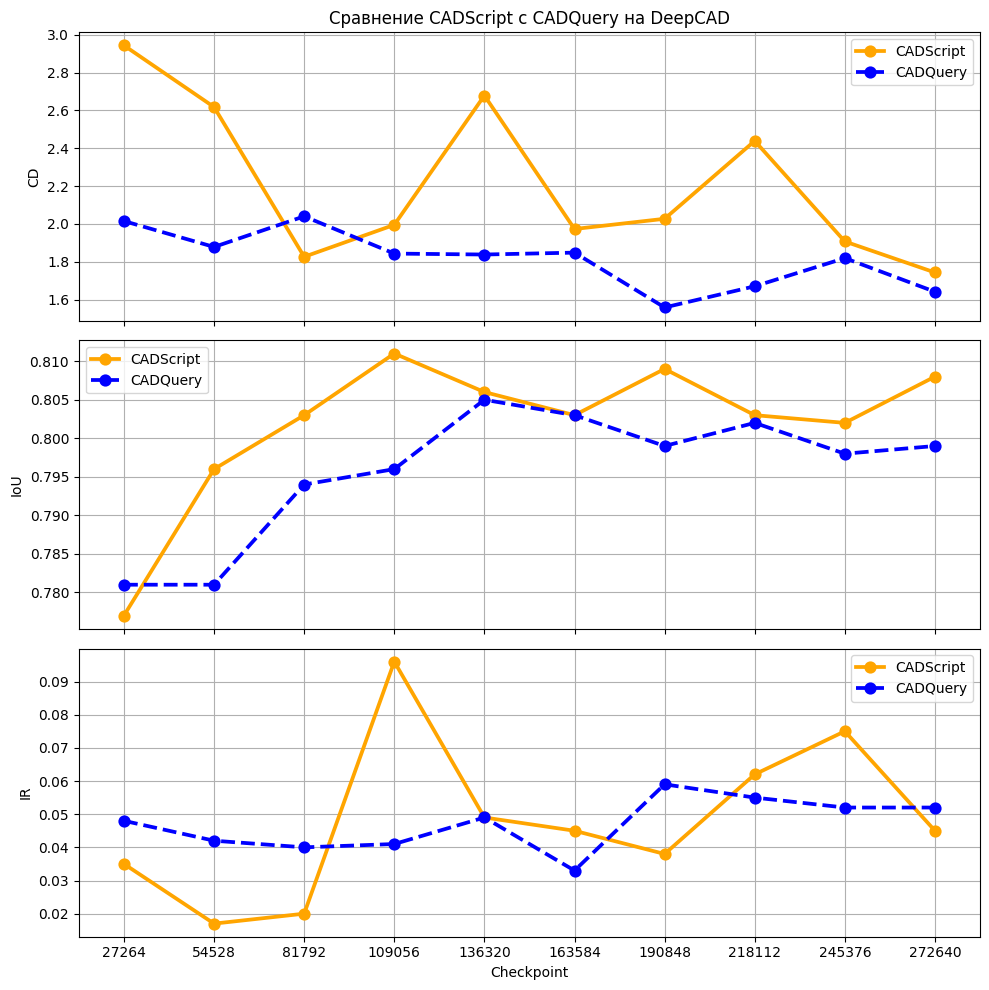
\includegraphics[width=\linewidth]{formats/formats_deepcad.png}
        \caption{DeepCAD}
    \end{subfigure}

    \vspace{1em}

    \begin{subfigure}{0.45\linewidth}
        \centering
        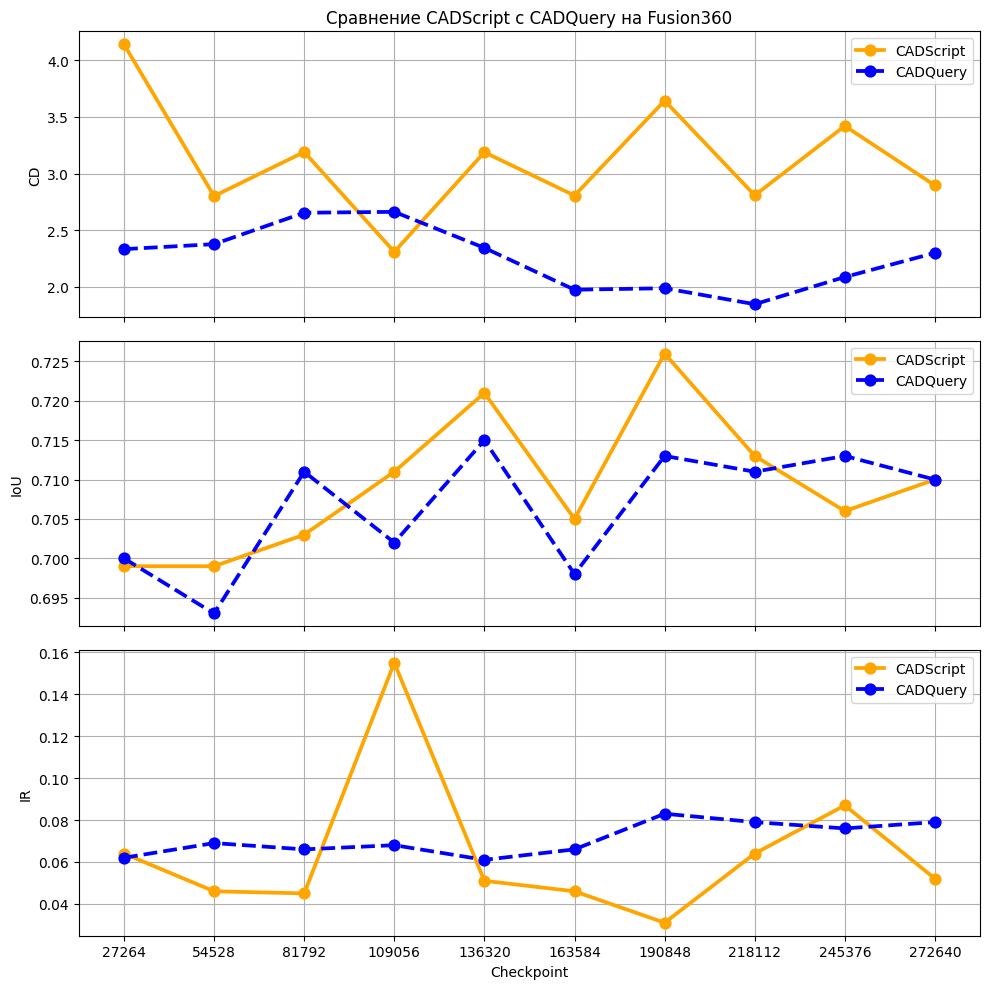
\includegraphics[width=\linewidth]{formats/formats_fusion360.png}
        \caption{Fusion360}
    \end{subfigure}
    \hfill
    \begin{subfigure}{0.45\linewidth}
        \centering
        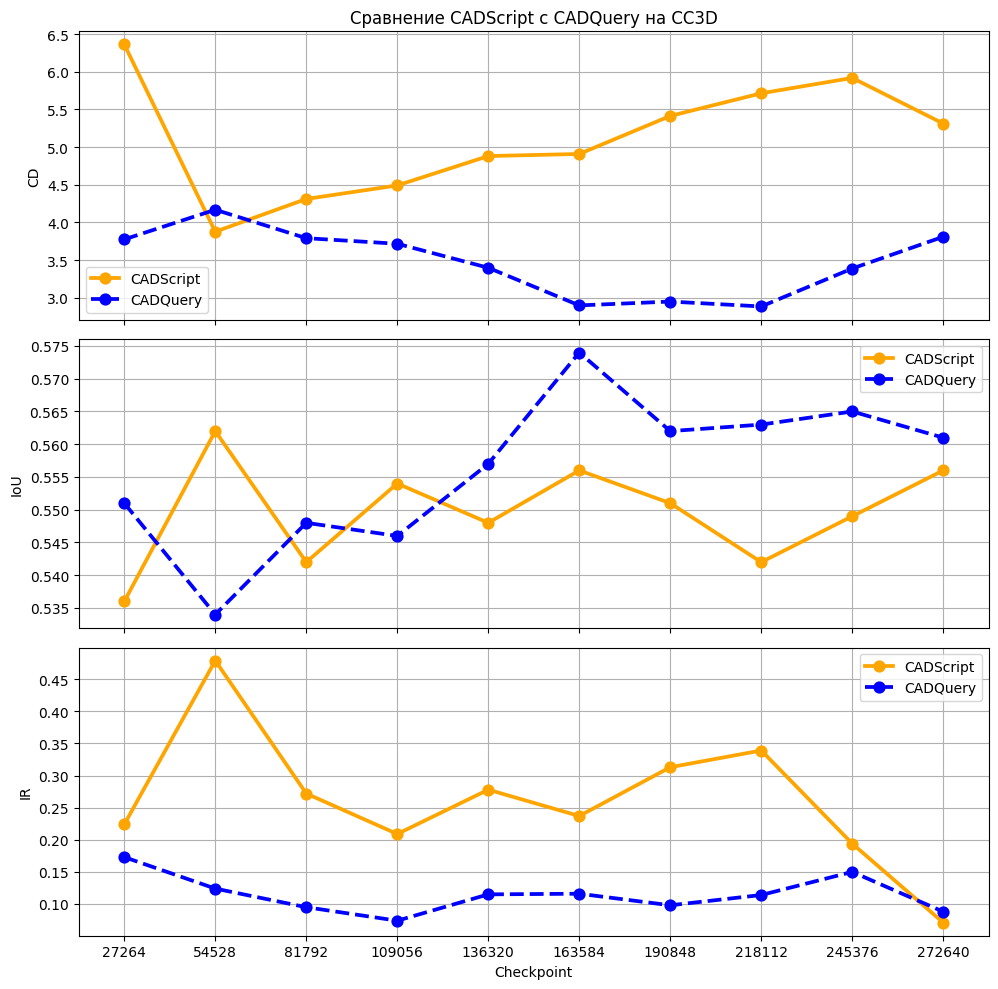
\includegraphics[width=\linewidth]{formats/formats_cc3d.png}
        \caption{CC3D}
    \end{subfigure}

    \caption{Результаты экспериментов на CAD-Recode, DeepCAD, Fusion360 и CC3D.
        Верхний график относится к метрике Chamfer Distance (CD) и чем меньше, тем лучше. Второй график Intersection over Union (IoU) чем больше, тем лучше.
        Последний относится к Invalid Rate (IR) и чем меньше, тем лушче. CD и IoU подсчитаны только на валидных генерациях}
    \label{fig:exp1}
\end{figure}

Из графика валидации на CADRecode мы можем сделать вывод, что оба формата успешно выучивают train данные и на синтетических данных дают по сути одинаковые результаты, разница между которыми крайне мала.
На остальных графиках виден четкий тренд: CADScript дает всегда больше Chamfer Distance, чем CADQuery на реальных датасетах DeepCAD, Fusion360 и CC3D.
По метрике Intersection over Union сделать четкого вывода нельзя: разница на Fusion360 и DeepCAD настолько мала, что больше похожа на дисперсию экперимента, нежели на тренд, хотя на DeepCAD CADScript показал лучше результаты.
Однако на самом сложном датасете CC3D CADScript явно работает хуже.

По Invalid Rate также ничего конкретного нельзя утверждать, кроме как на датасете CC3D

На самом деле именно CC3D показывает проигрыш CADScript перед CADQuery. Однако CADQuery тоже не показывает хорошие метрики на подобном датасете.
Вероятно, проигрыш CADScript перед CADQuery на топологии такой высокой сложности заключается в отсутствии у CADScript базовых макросов для создания бокса или цилиндра, которые есть у CADQuery.
И в то время когда CADQuery приближает сложную топологию простыми примитивами CADScript пытается сделать сложный loop. Также различия могут быть вызваны претрейном Qwen на CADQuery, хотя вероятность этого не высока.

Однако если мы даже понимаем, что CADSсript проигрывает CADQuery, мы не может сказать конкретно что он хуже делает.
Так мы плавно переходим к проблеме, что так как отсутствуют метрики или валидационные сеты, которые бы оценивали способность модели на какие то операции.

\subsection{Валидационный сет SketchGraph}

В статье \texttt{Computer--Aided Design as Language}~\cite{ganin21_cadlanguage} авторы описывают модель для генерации CAD-эскизов. Архитектура их решения не представляет интереса в рамках данного изложения, однако собранные ими данные оказываются практически полезны.
Для формирования датасета исследователи использовали репозиторий документов, находящихся в открытом доступе на платформе Onshape (Onshape Developers). Результирующий набор данных представлен в виде последовательностей токенов, описывающих геометрические примитивы и отношения между ними (constraints). Это ещё один формат представления скетчей, дополнительно к формату profile-loop.

Конструкции constraints позволяют описывать сложные эскизы значительно меньшим количеством символов. На рисунке~\ref{fig:constraint} приведены примеры MirrorConstraint (зеркалирование), TangentConstraint (касательная), OrthogonalConstraint (перпендикуляр) и CoincidentConstraint (совпадение). Благодаря им, даже без явного указания координат, можно реализовать столь сложную фигуру, как сердце.

\begin{figure}[h!]
    \centering
    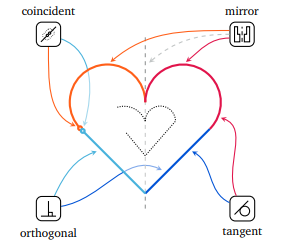
\includegraphics[width=0.5\textwidth]{constraint.png}
    \caption{Примеры constraints}
    \label{fig:constraint}
\end{figure}

Однако не все скетчи оказываются валидными для применения операции Extrude. На рисунке~\ref{fig:sketchgraph} видно, что в вариантах \ref{fig:sg1} и~\ref{fig:sg2} нельзя однозначно определить, что именно является вырезом из внешнего контура.

\begin{figure}[h!]
    \centering
    \begin{subfigure}[b]{0.3\textwidth}
        \centering
        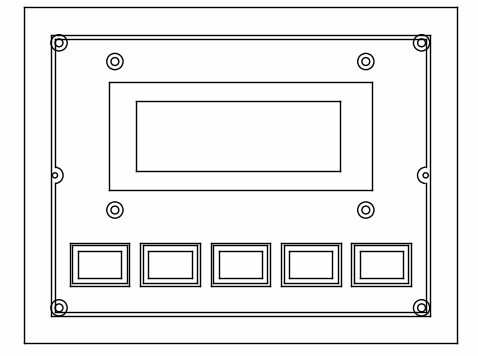
\includegraphics[width=\textwidth]{sg1.png}
        \caption{}
        \label{fig:sg1}
    \end{subfigure}
    \hfill
    \begin{subfigure}[b]{0.3\textwidth}
        \centering
        
\includegraphics[width=\textwidth]{sg2.png}
        \caption{}
        \label{fig:sg2}
    \end{subfigure}
    \hfill
    \begin{subfigure}[b]{0.3\textwidth}
        \centering
        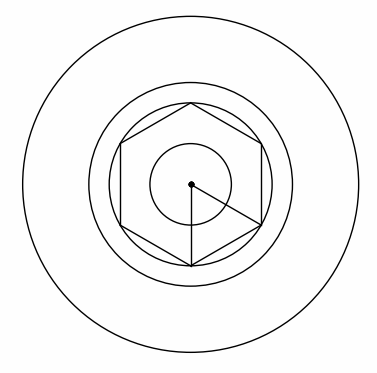
\includegraphics[width=\textwidth]{sg3.png}
        \caption{}
        \label{fig:sg3}
    \end{subfigure}
    \caption{Примеры скетчей из SketchGraph}
    \label{fig:sketchgraph}
\end{figure}

Чтобы решить эту проблему, можно взять все возможные замкнутые контуры (loop) в SketchGraph и выделить их подмножества, которые образуют валидный profile. Затем остаётся лишь перевести constraints в парадигму loop-profile, и мы получим валидные скетчи, которые можно сохранить в формате CADAxt.

Благодаря интеграции CADAxt с синтетическим генератором возможно выполнить экструдирование полученных эскизов. Таким образом формируется набор 3D-моделей, которые получены при помощи рисования скетчей различной сложности с последующей операцией Extrude.

Эти 3D-модели разделяют на три класса по уровню сложности:
\begin{enumerate}
    \item Простые: количество граней в интервале $(5, 15]$.
    \item Средние: количество граней в интервале $(15, 30]$.
    \item Сложные: количество граней в интервале $(30, 50]$.
\end{enumerate}

В итоге получается набор 3D-моделей, созданных одной операцией Extrude и разбитых на три класса. На рисунке~\ref{fig:sketchgraph_set} показан пример такого набора: слева~направо приведено по 9 представителей каждого класса от сложных к простым.

\begin{figure}[h!]
    \centering
    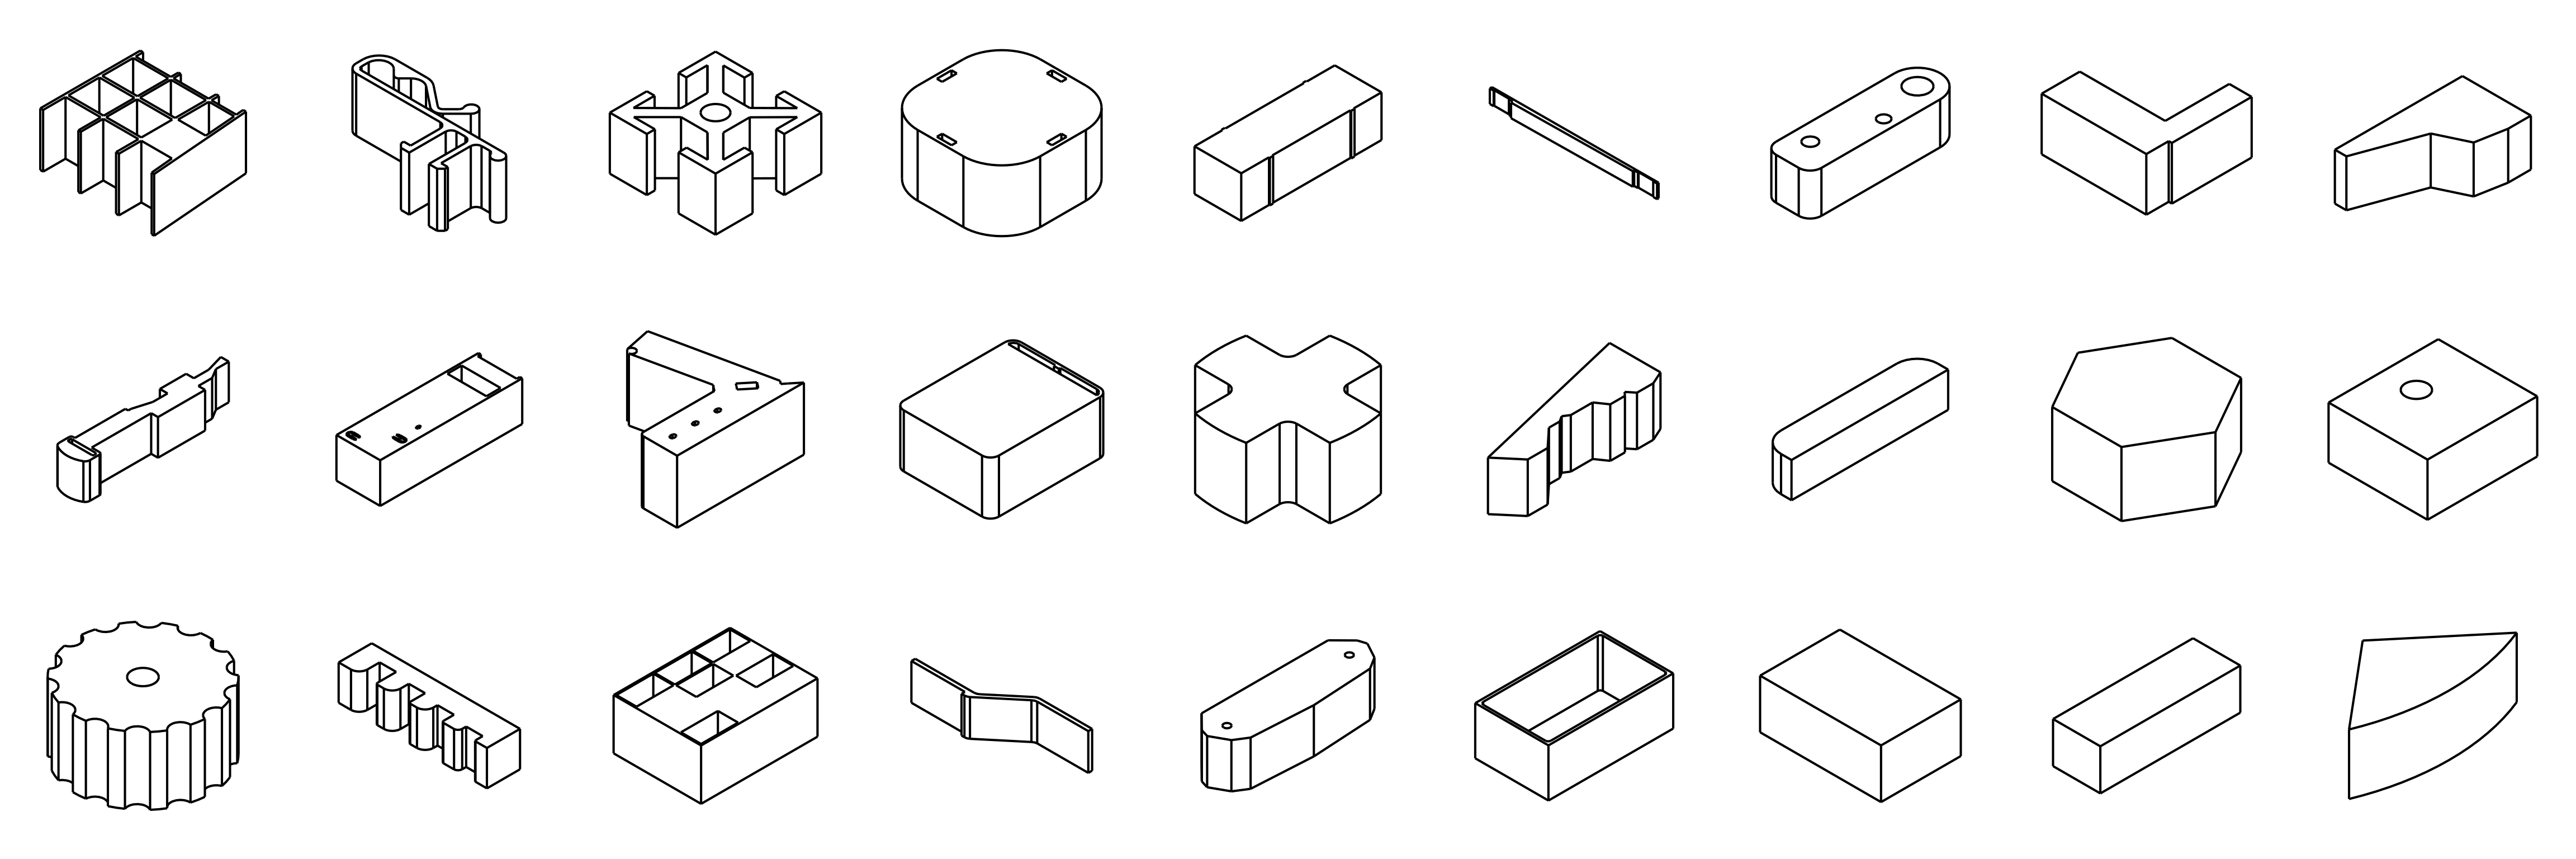
\includegraphics[width=\textwidth]{sketchgraph_set.png}
    \caption{Валидационный сет SketchGraph: примеры 3D-моделей, распределённых по сложности (сложные, средние, простые).}
    \label{fig:sketchgraph_set}
\end{figure}

Основная задача данного валидационного набора:
\begin{enumerate}
    \item Проверить способность модели воспроизводить представленные 3D-модели за одну операцию Extrude.
    \item Оценить, как модель справляется с топологиями разной сложности.
\end{enumerate}

\paragraph{Сравнение CADScript и CADQuery на SketchGraph}

Теперь можно проверить, насколько эффективно наши два представления (CADScript и CADQuery) способны рисовать скетчи.

\begin{figure}[h!]
    \centering
    \begin{subfigure}{0.45\linewidth}
        \centering
        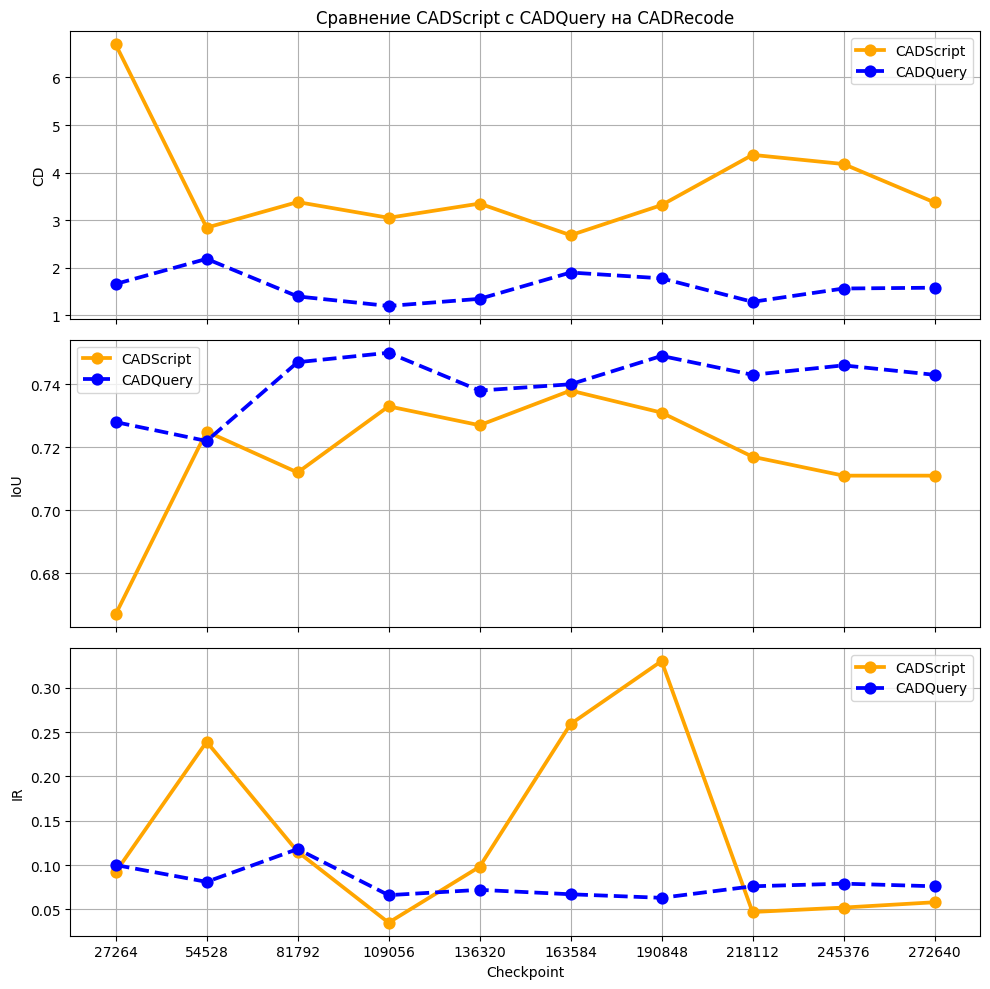
\includegraphics[width=\linewidth]{formats/formats_sketchgraph.png}
        \caption{На всём наборе данных}
    \end{subfigure}
    \hfill
    \begin{subfigure}{0.45\linewidth}
        \centering
        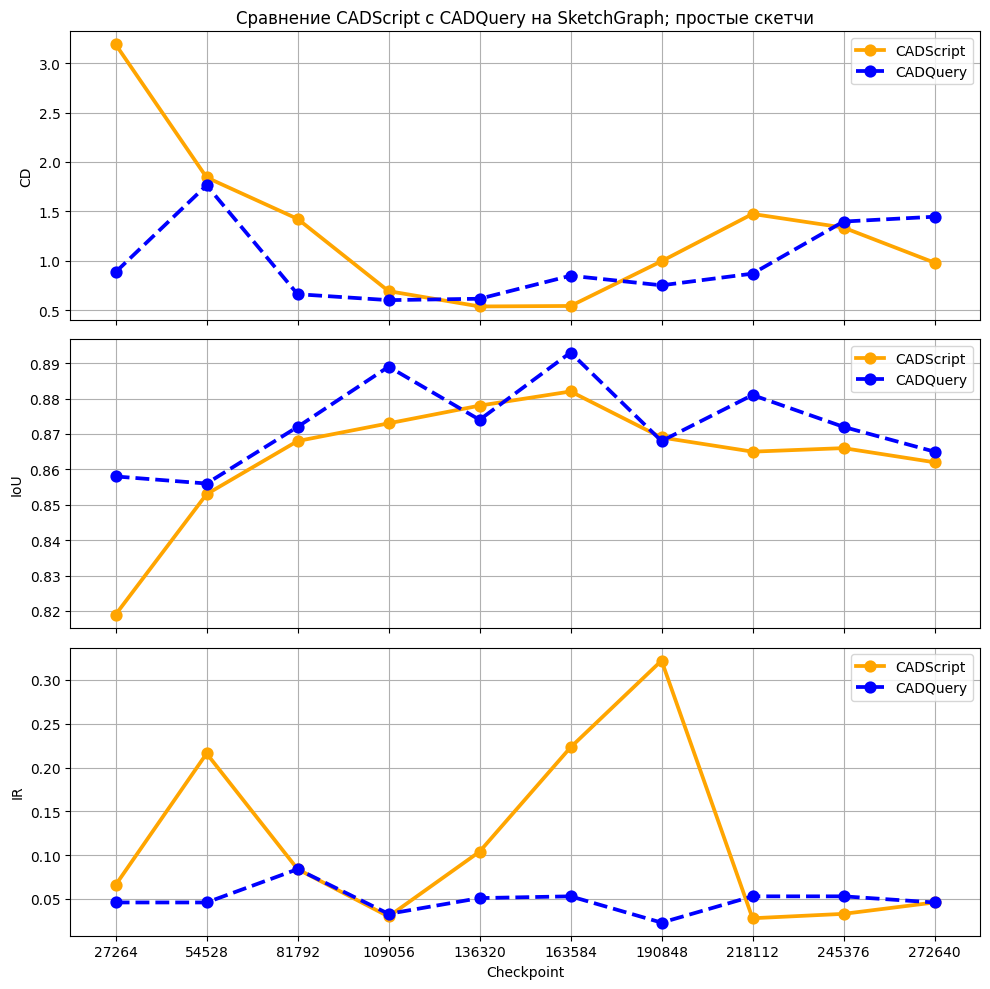
\includegraphics[width=\linewidth]{formats/formats_sketchgraph_easy.png}
        \caption{Простые скетчи}
    \end{subfigure}

    \vspace{1em}

    \begin{subfigure}{0.45\linewidth}
        \centering
        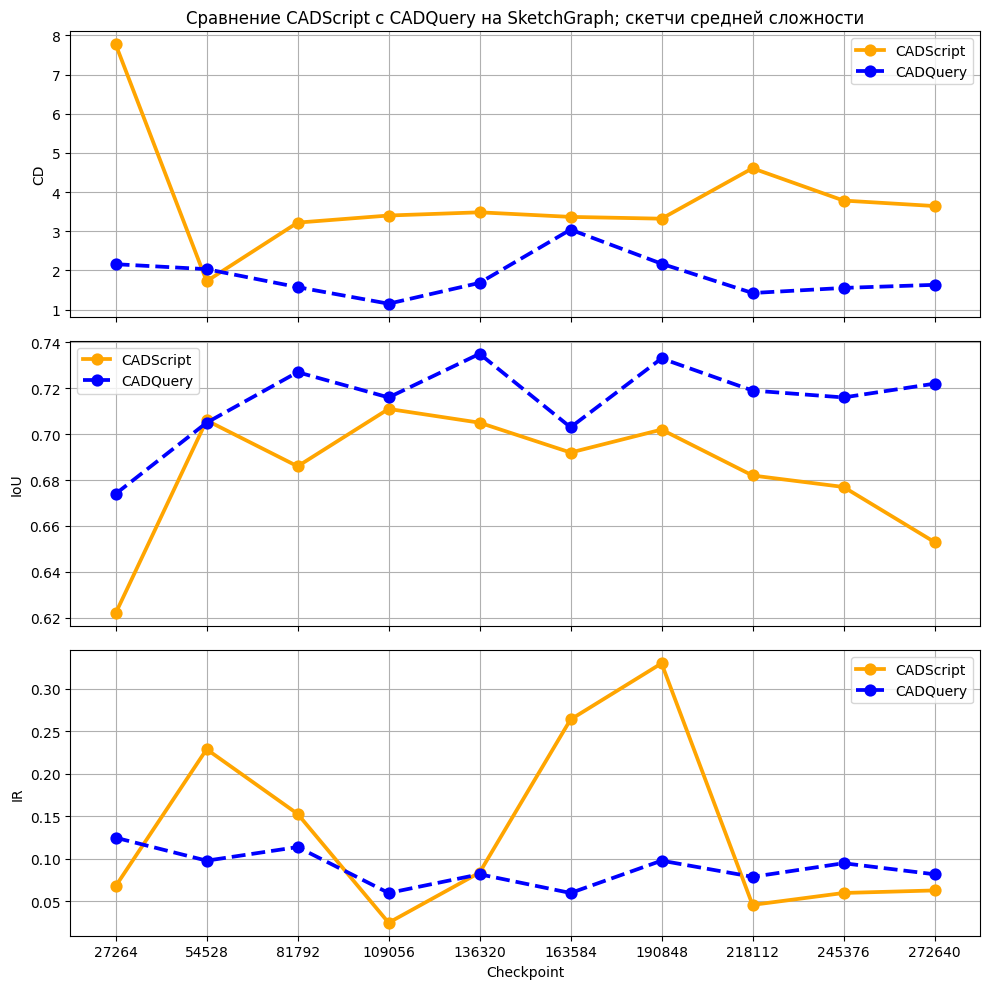
\includegraphics[width=\linewidth]{formats/formats_sketchgraph_medium.png}
        \caption{Скетчи средней сложности}
    \end{subfigure}
    \hfill
    \begin{subfigure}{0.45\linewidth}
        \centering
        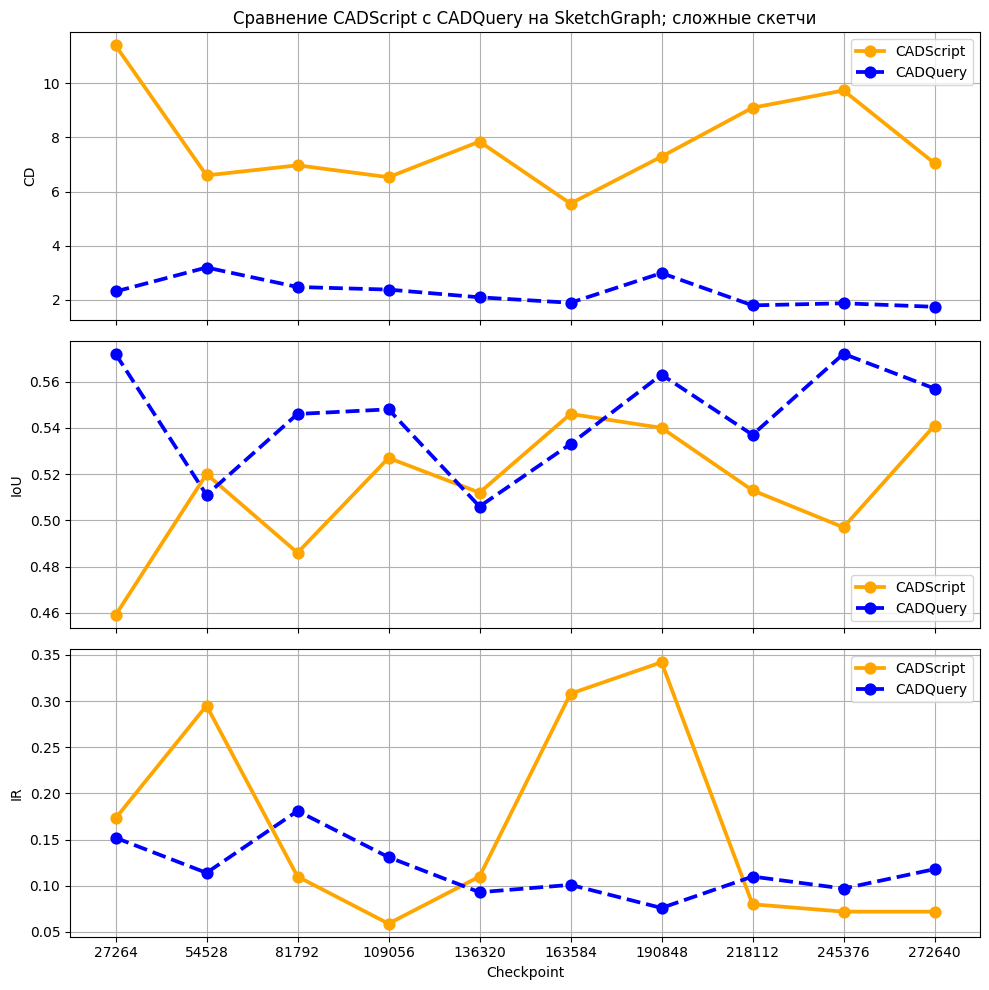
\includegraphics[width=\linewidth]{formats/formats_sketchgraph_hard.png}
        \caption{Сложные скетчи}
    \end{subfigure}

    \caption{Результаты экспериментов на SketchGraph и на трёх классах по уровню сложности топологии.
        Верхний график иллюстрирует метрику Chamfer Distance (CD), где меньшее значение лучше.
        Второй график --- Intersection over Union (IoU), где большее значение лучше.
        Третий график --- Invalid Rate (IR), где меньшее значение лучше.
        Метрики CD и IoU подсчитаны только на валидных генерациях.}
    \label{fig:exp2}
\end{figure}

Из графиков (рис.~\ref{fig:exp2}) хорошо видно, что на простых скетчах результаты CADScript и CADQuery сопоставимы. Однако на средних и сложных скетчах CADScript уступает CADQuery по метрикам CD и IoU, а показатель Invalid Rate сильно колеблется. Может возникнуть мысль, что CADQuery просто приближает топологию (за счёт большого числа простых команд) и поэтому показывает более высокие результаты, тогда как CADScript действительно старается точно воспроизводить скетчи. Или же CADQuery всегда использует простейшие макросы (cylinder/box) и, благодаря этому, повышает свои показатели.

Чтобы разобраться в этом, введём две дополнительные метрики:
\begin{enumerate}
    \item Extrude Mean (EM) --- среднее количество операций extrude.
    \item Base Extrude Ratio (BER) --- отношение числа простейших макросов (cylinder и
          box) у CADQuery ко всем его командам extrude.
\end{enumerate}

По этим метрикам получены следующие результаты:

\begin{figure}[h!]
    \centering
    \begin{subfigure}{0.45\linewidth}
        \centering
        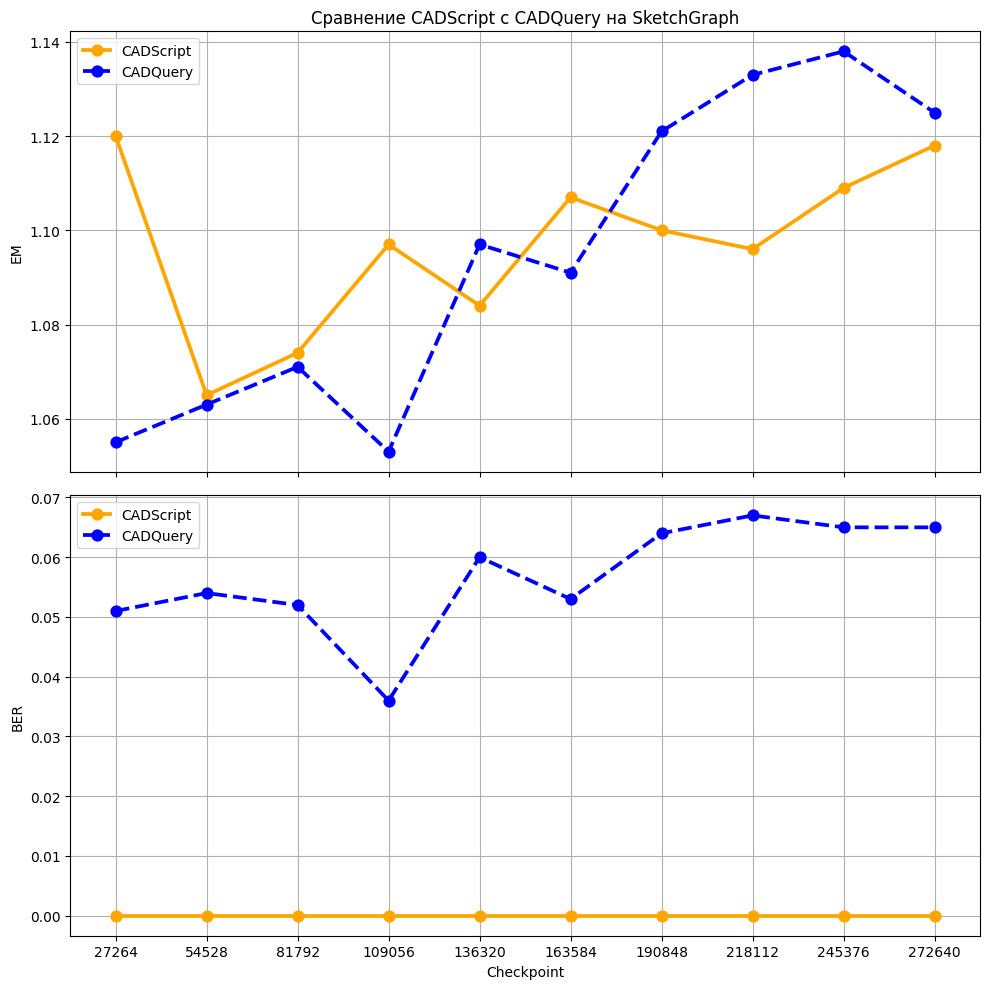
\includegraphics[width=\linewidth]{formats/format_em.png}
        \caption{На всём наборе данных}
    \end{subfigure}
    \hfill
    \begin{subfigure}{0.45\linewidth}
        \centering
        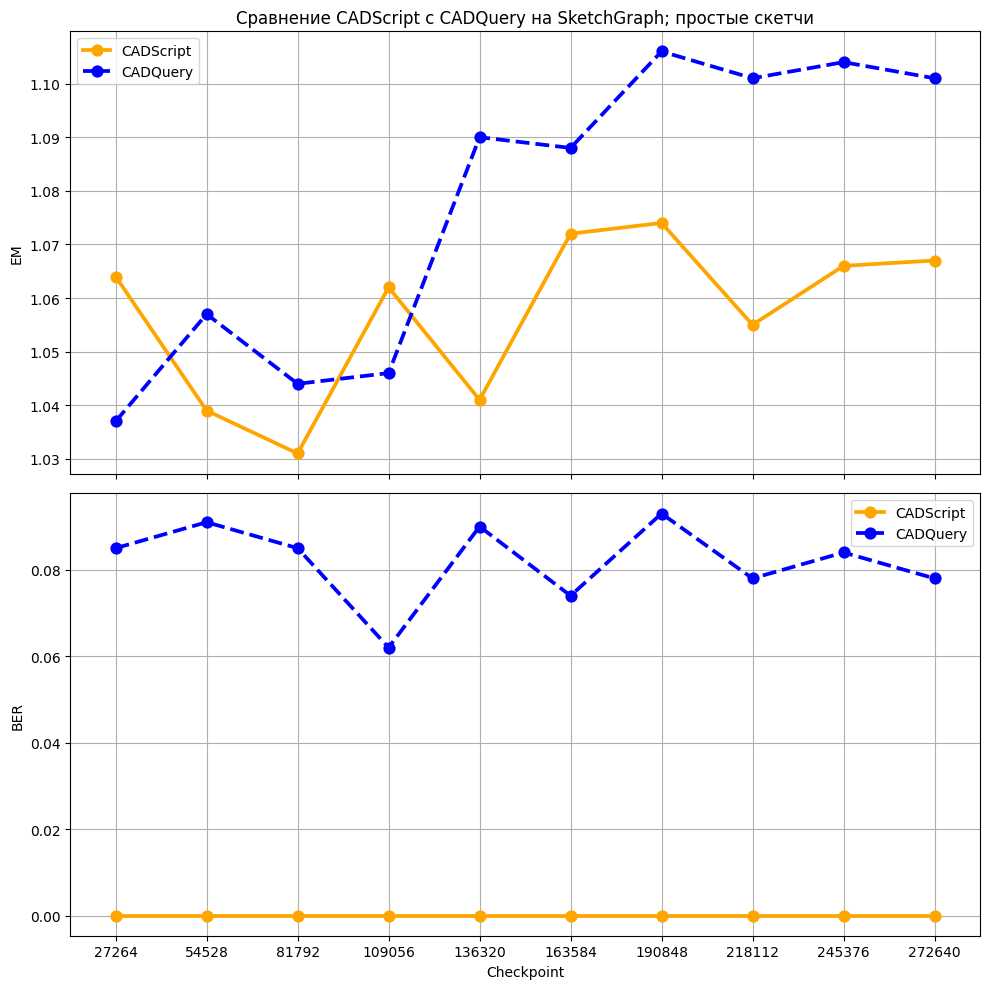
\includegraphics[width=\linewidth]{formats/format_em_e.png}
        \caption{Простые скетчи}
    \end{subfigure}

    \vspace{1em}

    \begin{subfigure}{0.45\linewidth}
        \centering
        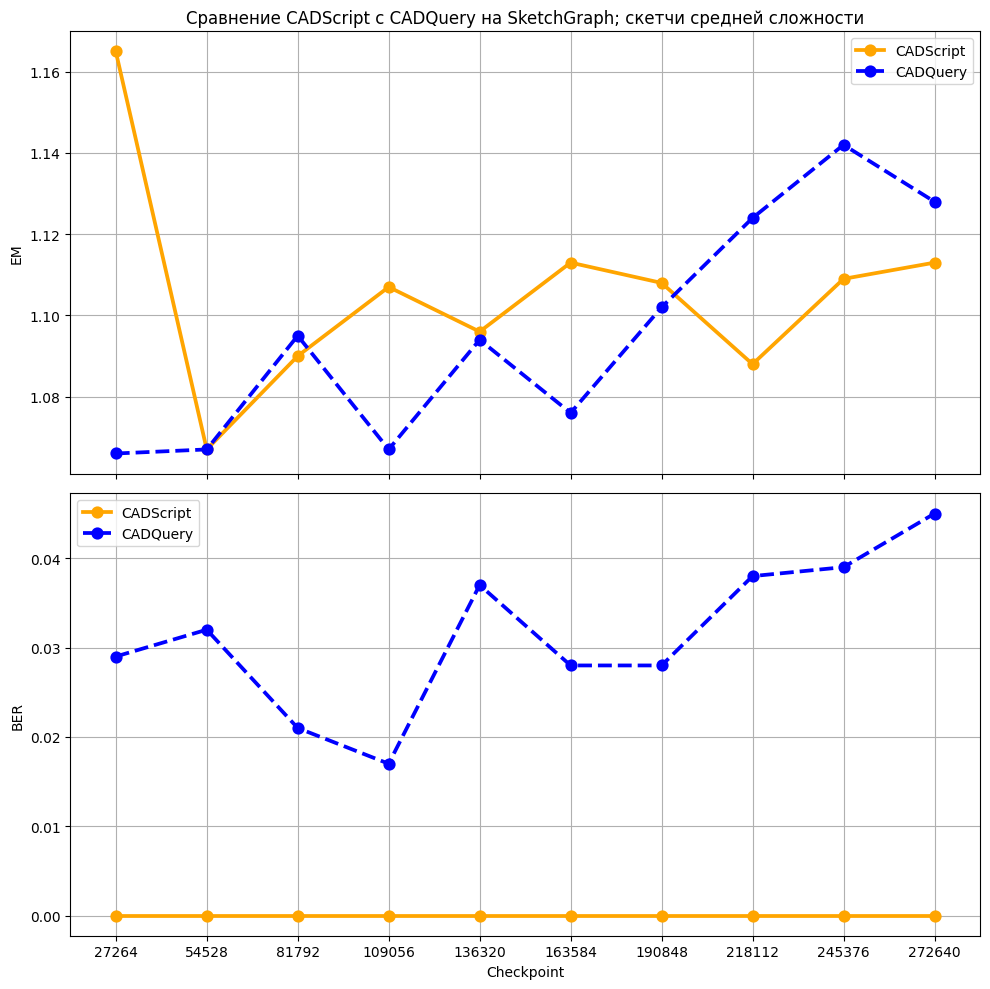
\includegraphics[width=\linewidth]{formats/format_em_m.png}
        \caption{Скетчи средней сложности}
    \end{subfigure}
    \hfill
    \begin{subfigure}{0.45\linewidth}
        \centering
        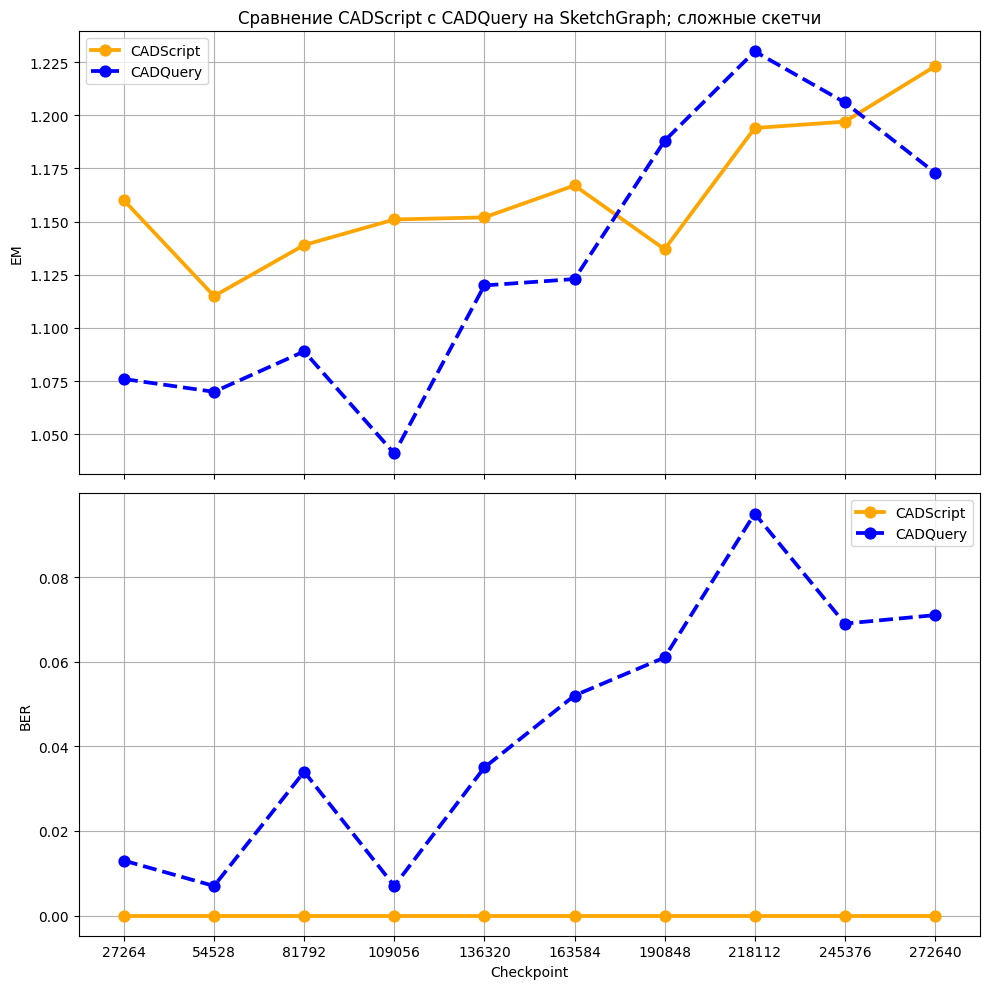
\includegraphics[width=\linewidth]{formats/format_em_h.png}
        \caption{Сложные скетчи}
    \end{subfigure}

    \caption{Результаты по метрикам Extrude Mean (EM) и Base Extrude Ratio (BER) на SketchGraph и на трёх классах по уровню сложности топологии.
        EM (верхний график) показывает среднее число команд extrude (чем меньше, тем лучше).
        BER (нижний график) отражает долю простейших макросов (cylinder или box) у CADQuery, и желательно, чтобы она не была слишком большой.}
    \label{fig:exp3}
\end{figure}

Из рис.~\ref{fig:exp3} видно, что CADQuery и CADScript в среднем используют сопоставимое число команд extrude, близкое к единице. При этом доля простейших макросов у CADQuery не превышает 9\,\%,
то есть CADQuery не злоупотребляет такими командами. Следовательно, CADQuery действительно лучше справляется с задачей рисования скетчей, чем CADScript.
Причиной этому может служить то, что в CADScript требуется явное задание описания Loop, в то время как в CADQuery оно происходит неявно.

Таким образом, формат CADQuery предпочтительнее формата CADScript: на реальных данных он дает меньшие значения метрики CD и лучше справляется с задачей рисования скетчей.

\newpage

\subsection{Тестирование экспериментов на SketchGraph}

Набор данных SketchGraph служит удобным средством для валидации и сравнения новых архитектур. Авторы работы CADRille применили дообучение с подкреплением (RL finetune) к уже обученной модели, основанной на данных DeepCAD и Fusion360. Для этого они использовали метод GRPO, функция потерь которого описывается соответствующим лоссом. Их основной целью было минимизировать показатель Invalid Rate (IR), не снижая метрику Intersection over Union (IoU). Введённая ими функция вознаграждения (reward) предполагала штраф в \(-10\) за несгенерированный семпл и вознаграждение в размере \(+ \mathrm{iou} \times 10\) за успешно сгенерированный.

Хотя такая схема действительно улучшила результаты на датасетах DeepCAD и Fusion360, концептуально она может привести к поведению, при котором модель старается генерировать упрощённую топологию и постепенно «доращивать» её до итога (напоминающее «покадровое» приближение). При таком подходе модель не получает штрафов за IR и постепенно учится повышать IoU. Поэтому важно проверить, что при таком дообучении модель не утрачивает способность корректно рисовать сложные скетчи.

В своих экспериментах я обучал модель CADRecode по схеме RL finetune с использованием GRPO, как в работе авторов CADRille. Обучение длилось 4 дня на 8 GPU H100 на подвыборке из 10\,000 семплов (20 эпох). Итоговые результаты представлены на рисунке~\ref{fig:exp4}.

\newpage
\begin{figure}[h!]
    \centering
    \begin{subfigure}{0.4\linewidth}
        \centering
        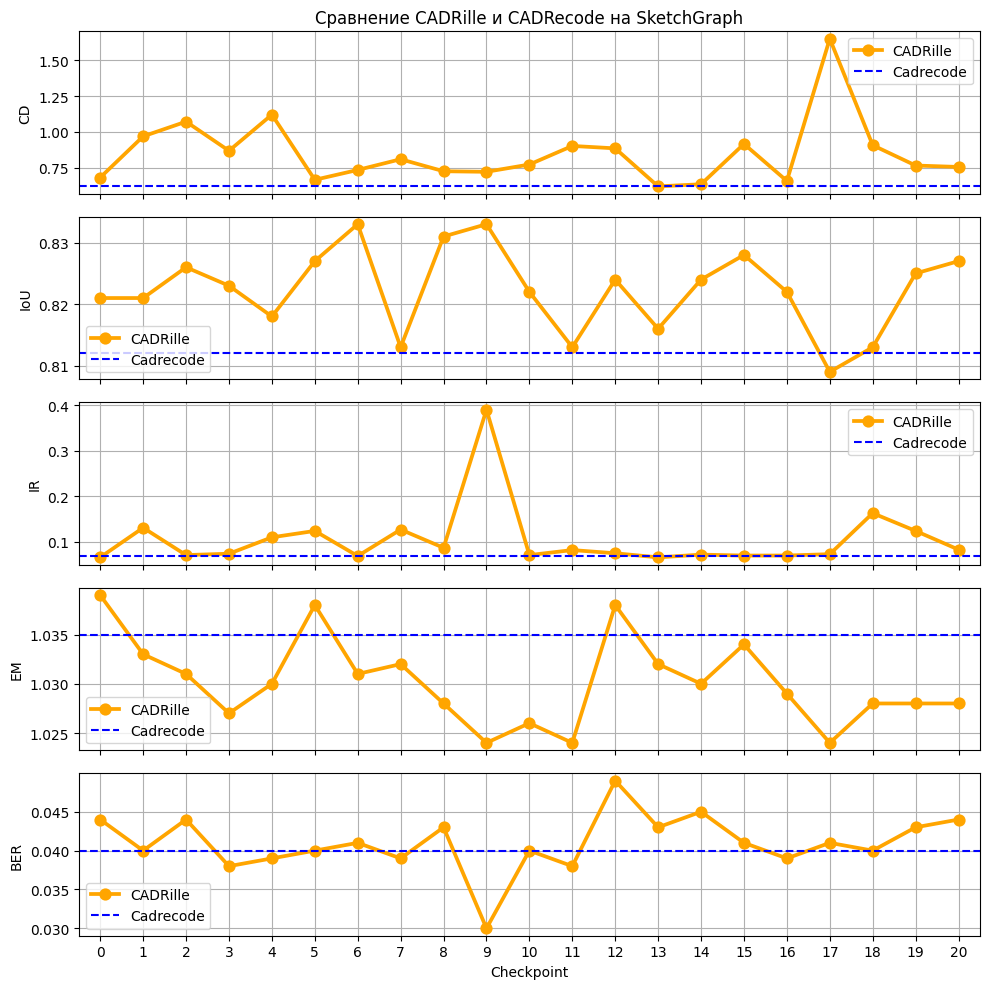
\includegraphics[width=\linewidth]{cadrille_sketchgraph.png}
        \caption{На всём наборе данных}
    \end{subfigure}
    \hfill
    \begin{subfigure}{0.4\linewidth}
        \centering
        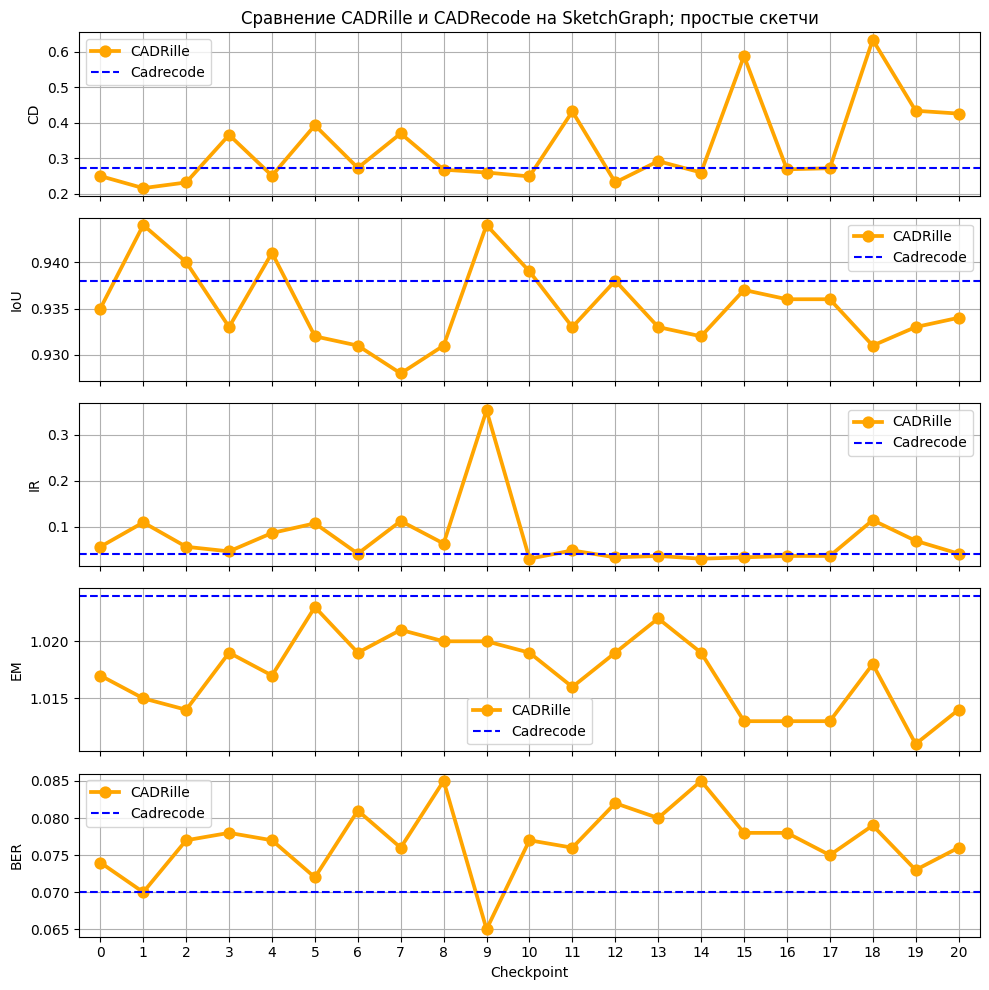
\includegraphics[width=\linewidth]{cadrille_sketchgraph_easy.png}
        \caption{Простые скетчи}
    \end{subfigure}

    \vspace{1em}

    \begin{subfigure}{0.4\linewidth}
        \centering
        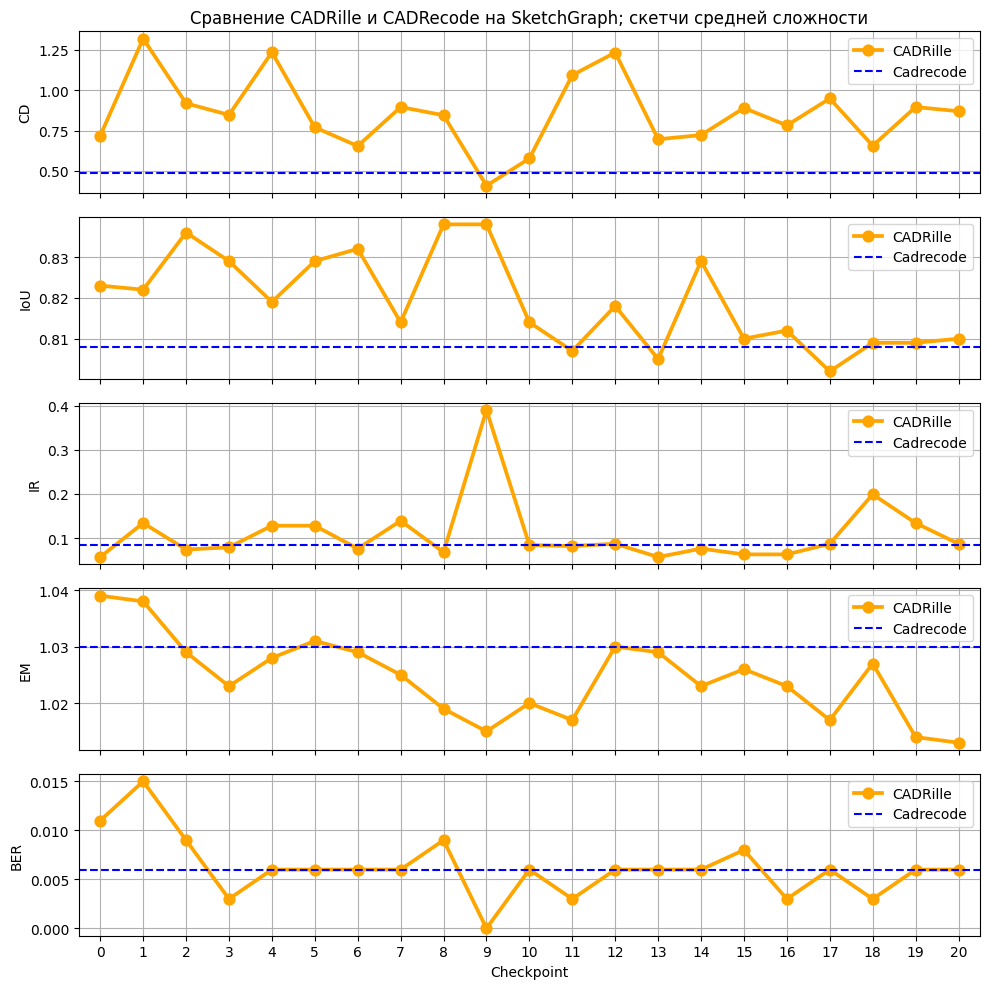
\includegraphics[width=\linewidth]{cadrille_sketchgraph_medium.png}
        \caption{Скетчи средней сложности}
    \end{subfigure}
    \hfill
    \begin{subfigure}{0.4\linewidth}
        \centering
        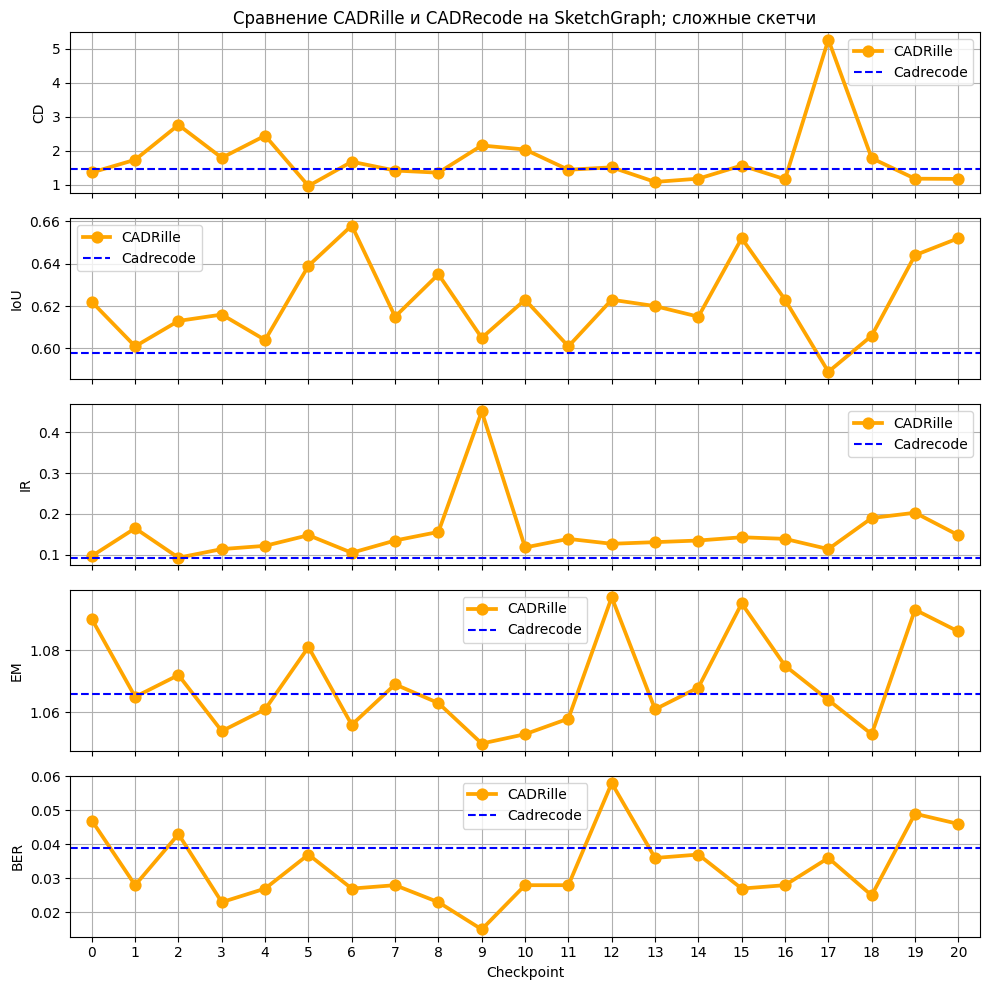
\includegraphics[width=\linewidth]{cadrille_sketchgraph_hard.png}
        \caption{Сложные скетчи}
    \end{subfigure}

    \caption{Результаты по метрикам CADRille с моделью CADRecode на SketchGraph и на трёх классах, разделённых по уровню сложности топологии.
        Верхняя диаграмма иллюстрирует метрику Chamfer Distance (CD), где меньшее значение лучше.
        Вторая диаграмма показывает Intersection over Union (IoU), где большее значение лучше.
        Третья диаграмма отражает показатель Invalid Rate (IR), где меньшее значение лучше.
        Метрики CD и IoU вычисляются только на валидных генерациях.
        EM (верхняя диаграмма) — это среднее число команд extrude (чем оно меньше, тем лучше).
        BER (нижняя диаграмма) — доля простейших макросов (cylinder или box) в среде CADQuery; желательно, чтобы это значение не было слишком высоким.}
    \label{fig:exp4}
\end{figure}

По результатам можно увидеть, что у CADRille растёт метрика IoU, а на скетчах лёгкого и среднего уровня наблюдается снижение количества команд \texttt{Extrude}.
Таким образом, подход CADRille не ухудшает способность CADRecode корректно рисовать скетчи, при этом повышая обобщающую способность модели.

\subsection{Синтетический датасет на SketchGraph.}
После интеграции скетчей из SketchGraph в пайплайн генератора CADRecode появилась возможность сгенерировать новый датасет и обучить на нём модель, сравнив результаты с датасетом на синтетических скетчах. Предполагается, что такой подход внесёт дополнительный индуктивный байас и улучшит метрики на всех датасетах.

Для эксперимента было сгенерировано два датасета на пайплайне генератора CADRecode, различающихся только типом скетчей. Обучение на каждом из них проходило на четырёх GPU H100 с размером батча 9 в течение 10 эпох. Время обучения обоих вариантов оказалось одинаковым.

\begin{figure}[h!]
    \centering
    \begin{subfigure}{0.45\linewidth}
        \centering
        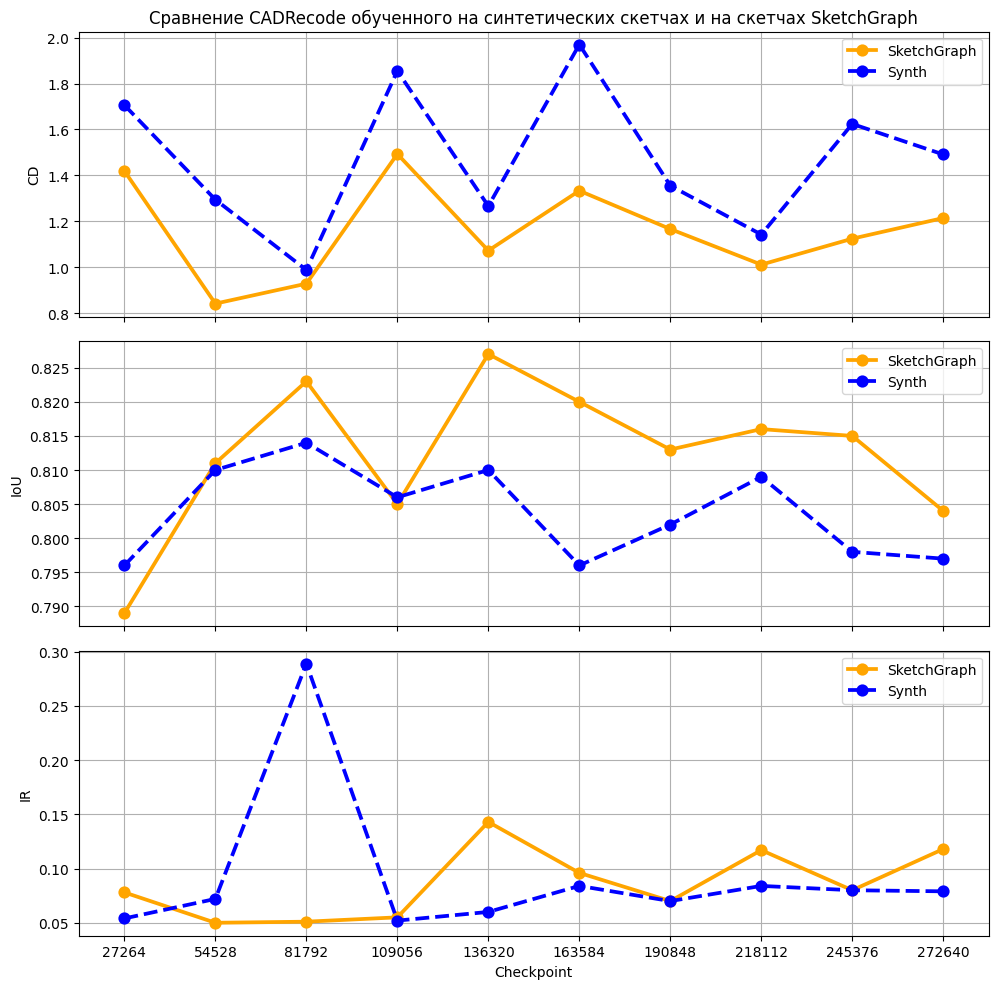
\includegraphics[width=\linewidth]{cadrecode_sg_deepcad.png}
        \caption{DeepCAD}
    \end{subfigure}
    \hfill
    \begin{subfigure}{0.45\linewidth}
        \centering
        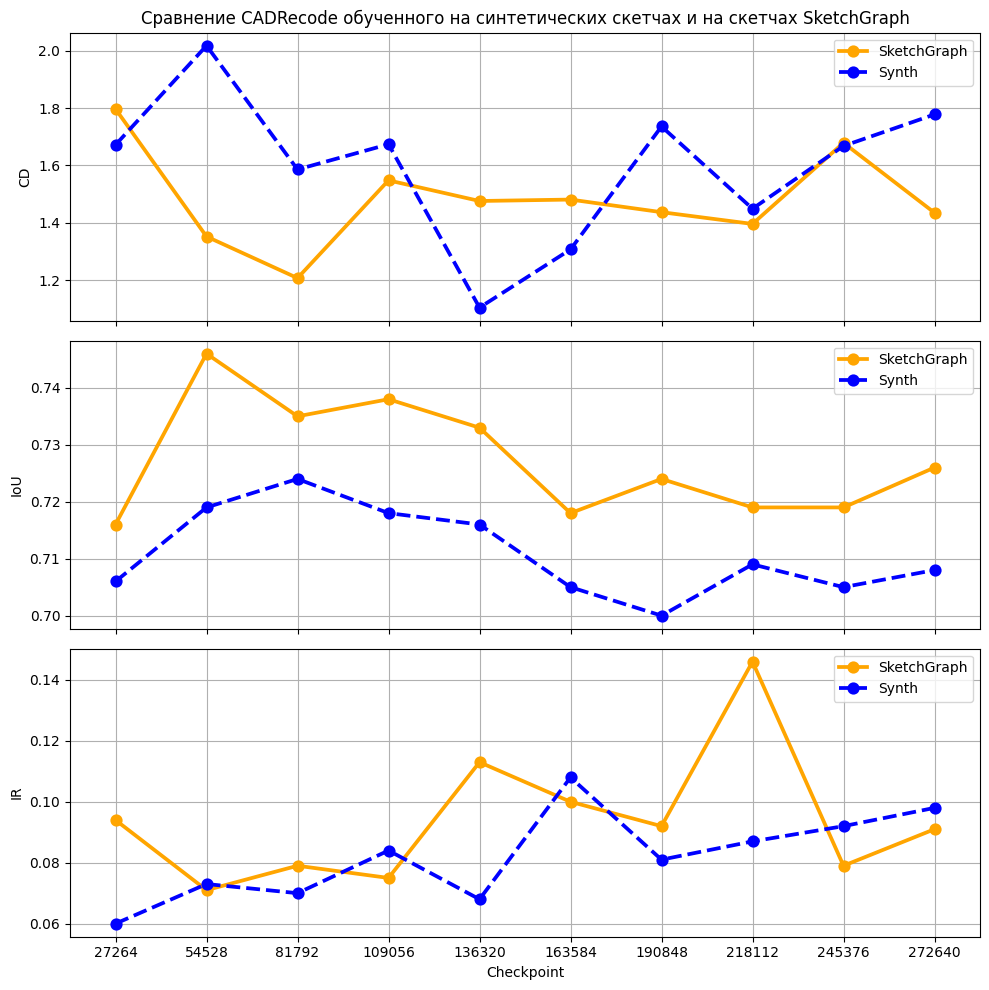
\includegraphics[width=\linewidth]{cadrecode_sg_fusion360.png}
        \caption{Fusion360}
    \end{subfigure}

    \vspace{1em}

    \begin{subfigure}{0.45\linewidth}
        \centering
        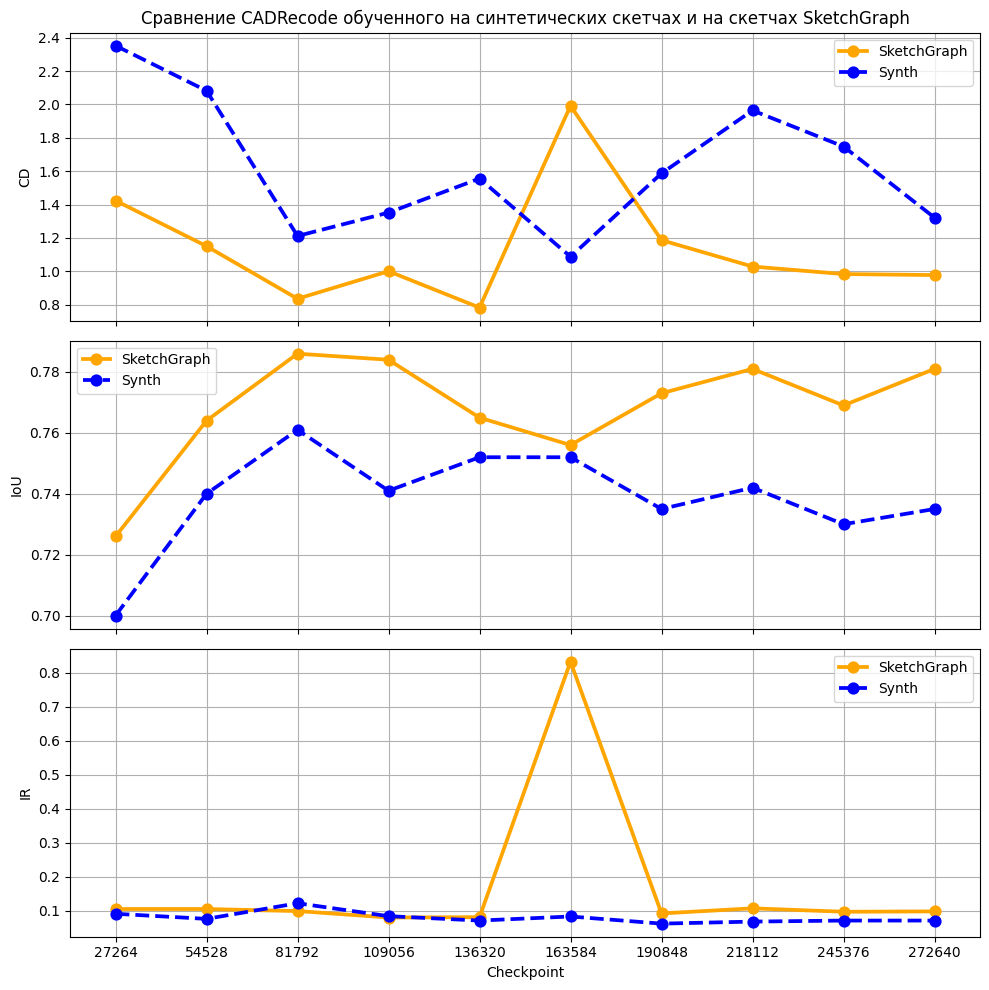
\includegraphics[width=\linewidth]{cadrecode_sg_sketchgraph.png}
        \caption{SketchGraph}
    \end{subfigure}
    \hfill
    \begin{subfigure}{0.45\linewidth}
        \centering
        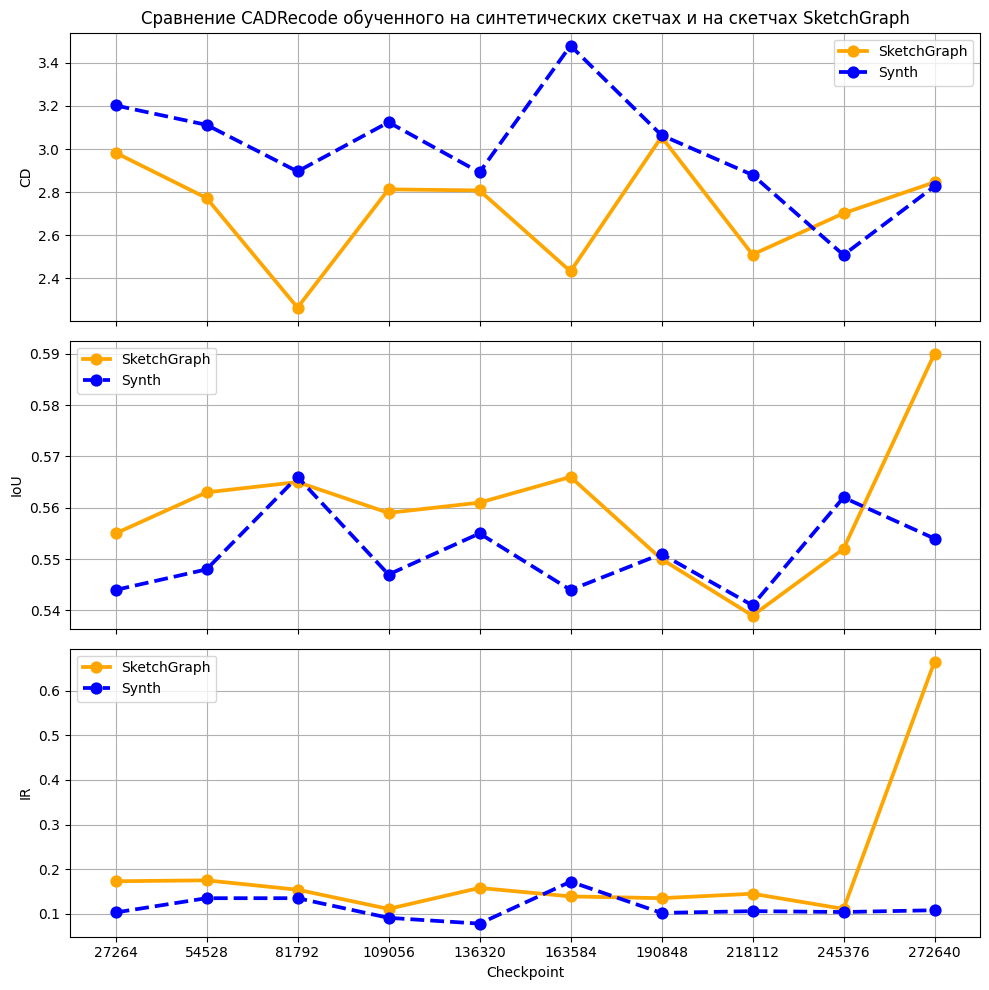
\includegraphics[width=\linewidth]{cadrecode_sg_cc3d.png}
        \caption{CC3D}
    \end{subfigure}

    \caption{Результаты экспериментов на DeepCAD, Fusion360, SketchGraph и CC3D.
        Верхний график показывает метрику Chamfer Distance (CD), где меньшие значения лучше.
        Второй график — Intersection over Union (IoU), где большие значения лучше.
        Последний график — Invalid Rate (IR), где меньшие значения лучше.
        CD и IoU подсчитаны только среди валидных генераций.}
    \label{fig:exp5}
\end{figure}

На рис.~\ref{fig:exp5} заметно, что модель, обученная на скетчах из SketchGraph, чаще демонстрирует более высокий IoU и меньший CD, что говорит об успешной интеграции данного подхода.
Сравним два лучших чекпоинта: модель на 81792-й итерации (скетчи из SketchGraph) и на 136320-й итерации (синтетические скетчи).

\begin{table}[h!]
    \centering
    \begin{tabular}{lccc}
        \toprule
        \textbf{Модель} & \textbf{CD}    & \textbf{IoU}   & \textbf{IR}    \\
        \midrule
        SketchGraph     & 1.207          & \textbf{0.735} & 0.079          \\
        Synth           & \textbf{1.104} & 0.716          & \textbf{0.068} \\
        \bottomrule
    \end{tabular}
    \caption{Результаты измерений на Fusion360.}
\end{table}

\begin{table}[h!]
    \centering
    \begin{tabular}{lccc}
        \toprule
        \textbf{Модель} & \textbf{CD}    & \textbf{IoU}   & \textbf{IR}    \\
        \midrule
        SketchGraph     & \textbf{0.928} & \textbf{0.823} & \textbf{0.051} \\
        Synth           & 1.266          & 0.810          & 0.060          \\
        \bottomrule
    \end{tabular}
    \caption{Результаты измерений на DeepCAD.}
\end{table}

\begin{table}[h!]
    \centering
    \begin{tabular}{lccc}
        \toprule
        \textbf{Модель} & \textbf{CD}    & \textbf{IoU}   & \textbf{IR}    \\
        \midrule
        SketchGraph     & \textbf{2.265} & \textbf{0.565} & 0.154          \\
        Synth           & 2.892          & 0.555          & \textbf{0.078} \\
        \bottomrule
    \end{tabular}
    \caption{Результаты измерений на CC3D.}
\end{table}

\begin{table}[h!]
    \centering
    \begin{tabular}{lccc}
        \toprule
        \textbf{Модель} & \textbf{CD}    & \textbf{IoU}   & \textbf{IR}    \\
        \midrule
        SketchGraph     & \textbf{0.836} & \textbf{0.786} & 0.099          \\
        Synth           & 1.556          & 0.752          & \textbf{0.071} \\
        \bottomrule
    \end{tabular}
    \caption{Результаты измерений на SketchGraph.}
\end{table}

Из таблиц видно, что модель, обученная на реальных скетчах, особенно хорошо проявляет себя на датасетах DeepCAD и SketchGraph. Вероятно, более сложные скетчи из Fusion360 и CC3D затрудняют процесс генерации, однако на DeepCAD и SketchGraph способность к более сложному рисованию становится ключевым фактором качества.

С другой стороны, на Fusion360 и CC3D нельзя однозначно утверждать превосходство одной модели над другой, в частности из-за отличий в Invalid Rate (IR).

Рассмотрим визуальное сравнение на датасете CC3D (рис.~\ref{fig:datasets1}).

\begin{figure}[h!]
    \centering
    
\includegraphics[width=\textwidth]{collage_with_gt_cc3d_synth.png}
    \caption*{Synth}
    \vspace{1em}
    
\includegraphics[width=\textwidth]{collage_with_gt_cc3d_sg.png}
    \caption*{SketchGraph}
    \caption{Визуальное сравнение результатов на CC3D.}
    \label{fig:datasets1}
\end{figure}

На данных примерах модель, обученная на реальных скетчах, лучше улавливает симметрию и демонстрирует аккуратные результаты, которые выглядят более редактируемыми.
В целом модель стала работать лучше, хотя систематически имеет более высокий Invalid Rate.
Вероятно, при применении RL-подхода (например, CADRille) этот недостаток можно компенсировать и улучшить метрики ещё заметнее.

\subsection{Будущая работа}

В данной работе используется генератор CADRecode, однако я веду разработку собсвенного генератора, который будет еще больше приближен к инженерным объектам за счет новых правил построения.
К сожалению, на данный момент, мой генератор имеет недоработки из-за чего обучение не проходит успешно

Также планируется внедрить изменения в архитектуру PointCloud модуля в CADRecode, а именно протестировать на различных PointCloudEncoder и подобрать оптимальное количество семплируемых точек для генерации

Конечно, также планируется поставить эксперименты с RL-finetune на синтетике со скетчами SketchGraph, а также провести эксперименты с другой reward функцией

\newpage
 %% Исследование и построение решения задачи
    \section{Заключение}
\label{sec:Chapter4} \index{Chapter4}

В ходе данной работы был сформирован валидационный набор скетчей на основе библиотеки SketchGraph, что позволило провести сравнительный анализ двух форматов представления данных: \texttt{CADScript} и \texttt{CADQuery}. Также был создан синтетический датасет, основанный на инженерных скетчах, и проведён эксперимент, в котором результаты, полученные с новым датасетом, сравнивались с исходными синтетическими данными.

Проведённый эксперимент продемонстрировал улучшение метрик \texttt{CD} и \texttt{IoU} при некотором увеличении показателя \texttt{IR}. Тем не менее, визуальный анализ подтверждает возрастание качества генерируемых скетчей, что указывает на эффективность предложенного подхода и его положительное влияние на работу модели.

\newpage
 %% Описание практической части
    % \input{parts/Chapter5.tex} %% Заключение

    %% НЕ ТРОГАЙТЕ!!!
    \nocite{*}
    \bibliography{references}

    %% в зависимости от надобности подключаем раздел "Приложение"
    % \newpage
    % \section*{Приложение}
\addcontentsline{toc}{section}{Приложение}
\label{sec:Apendix} \index{Apendix}

\begin{table}[]
	\caption{Сравнение CADScript и CADQuery на датасете CADRecode}
	\centering
	\begin{tabular}{ccccccccc}
		\hline
		\textbf{Checkpoint} & $CD\textsubscript{a}$ & $CD\textsubscript{v}$ & $CD\textsubscript{vv}$ & $IoU\textsubscript{a}$ & $IoU\textsubscript{v}$ & $IoU\textsubscript{vv}$ & $IR$          & format    \\
		\hline
		27264               & 71.10                 & 1.58                  & 1.49                   & 0.78                   & 0.83                   & 0.86                    & 0.06          & cadquery  \\
		27264               & 43.05                 & 4.71                  & 4.08                   & 0.75                   & 0.78                   & 0.80                    & 0.03          & cadscript \\
		54528               & 42.81                 & 1.88                  & 1.64                   & 0.81                   & 0.83                   & 0.89                    & 0.03          & cadquery  \\
		54528               & 34.84                 & 2.34                  & 2.32                   & 0.80                   & 0.82                   & 0.85                    & 0.03          & cadscript \\
		81792               & 51.87                 & 1.83                  & 1.35                   & 0.82                   & 0.86                   & 0.90                    & 0.04          & cadquery  \\
		81792               & \textbf{26.27}        & 1.61                  & 1.60                   & \textbf{1.19}          & \textbf{1.22}          & \textbf{1.26}           & \textbf{0.02} & cadscript \\
		109056              & 33.98                 & 2.33                  & 1.28                   & 0.83                   & 0.85                   & 0.90                    & 0.03          & cadquery  \\
		109056              & 32.18                 & 2.04                  & 2.04                   & 0.83                   & 0.85                   & 0.88                    & 0.03          & cadscript \\
		136320              & 31.66                 & 1.72                  & 1.65                   & 0.85                   & 0.87                   & 0.90                    & 0.03          & cadquery  \\
		136320              & 32.71                 & 1.57                  & 1.49                   & 0.83                   & 0.86                   & 0.88                    & 0.03          & cadscript \\
		163584              & 37.37                 & 1.71                  & 1.42                   & 0.85                   & 0.87                   & 0.91                    & 0.03          & cadquery  \\
		163584              & 49.27                 & 1.59                  & 1.50                   & 0.83                   & 0.87                   & 0.89                    & 0.04          & cadscript \\
		190848              & 27.86                 & 1.66                  & 1.37                   & 0.85                   & 0.86                   & 0.90                    & \textbf{0.02} & cadquery  \\
		190848              & 41.12                 & 1.91                  & 1.63                   & 0.85                   & 0.88                   & 0.90                    & 0.03          & cadscript \\
		218112              & 34.52                 & 1.63                  & 1.21                   & 0.85                   & 0.88                   & 0.91                    & 0.03          & cadquery  \\
		218112              & 57.30                 & 2.41                  & 2.15                   & 0.82                   & 0.86                   & 0.88                    & 0.05          & cadscript \\
		245376              & 44.39                 & 1.82                  & 1.33                   & 0.84                   & 0.87                   & 0.91                    & 0.04          & cadquery  \\
		245376              & 49.58                 & \textbf{1.22}         & \textbf{1.18}          & 0.84                   & 0.88                   & 0.90                    & 0.04          & cadscript \\
		272640              & 36.99                 & 1.70                  & 1.22                   & 0.84                   & 0.87                   & 0.91                    & 0.03          & cadquery  \\
		272640              & 37.40                 & 1.63                  & 1.45                   & 0.85                   & 0.88                   & 0.90                    & 0.03          & cadscript \\
		\hline
	\end{tabular}
\end{table}

\begin{table}[]
	\centering
	\caption{сравнение CADScript и CADQuery на датасете DeepCAD}
	\begin{tabular}{c c c c c c c c c}
		\hline
		\textbf{Checkpoint} & $CD\textsubscript{a}$ & $CD\textsubscript{v}$ & $CD\textsubscript{vv}$ & $IoU\textsubscript{a}$ & $IoU\textsubscript{v}$ & $IoU\textsubscript{vv}$ & $IR$          & format    \\
		\hline
		27264               & 55.92                 & 2.01                  & 1.54                   & 0.74                   & 0.78                   & 0.83                    & 0.05          & cadquery  \\
		27264               & 42.56                 & 2.94                  & 2.29                   & 0.75                   & 0.78                   & 0.81                    & 0.04          & cadscript \\
		54528               & 50.10                 & 1.88                  & 1.34                   & 0.75                   & 0.78                   & 0.83                    & 0.04          & cadquery  \\
		54528               & \textbf{21.21}        & 2.62                  & 1.76                   & 0.78                   & 0.80                   & 0.83                    & \textbf{0.02} & cadscript \\
		81792               & 48.93                 & 2.04                  & 1.34                   & 0.76                   & 0.79                   & 0.83                    & 0.04          & cadquery  \\
		81792               & 24.69                 & 1.83                  & 1.76                   & \textbf{0.79}          & 0.80                   & 0.83                    & \textbf{0.02} & cadscript \\
		109056              & 49.09                 & 1.84                  & 1.09                   & 0.76                   & 0.80                   & 0.84                    & 0.04          & cadquery  \\
		109056              & 109.47                & 1.99                  & 1.48                   & 0.73                   & \textbf{0.81}          & 0.83                    & 0.10          & cadscript \\
		136320              & 56.59                 & 1.84                  & \textbf{1.08}          & 0.77                   & \textbf{0.81}          & \textbf{0.85}           & 0.05          & cadquery  \\
		136320              & 58.88                 & 2.68                  & 2.20                   & 0.77                   & \textbf{0.81}          & 0.83                    & 0.05          & cadscript \\
		163584              & 40.35                 & 1.85                  & 1.49                   & 0.78                   & 0.80                   & 0.84                    & 0.03          & cadquery  \\
		163584              & 52.72                 & 1.97                  & 1.86                   & 0.77                   & 0.80                   & 0.84                    & 0.04          & cadscript \\
		190848              & 69.08                 & \textbf{1.56}         & 1.52                   & 0.75                   & 0.80                   & 0.84                    & 0.06          & cadquery  \\
		190848              & 44.64                 & 2.03                  & 1.60                   & 0.78                   & \textbf{0.81}          & 0.83                    & 0.04          & cadscript \\
		218112              & 63.77                 & 1.67                  & 1.31                   & 0.76                   & 0.80                   & \textbf{0.85}           & 0.06          & cadquery  \\
		218112              & 72.22                 & 2.44                  & 2.32                   & 0.75                   & 0.80                   & 0.82                    & 0.06          & cadscript \\
		245376              & 60.57                 & 1.82                  & 1.43                   & 0.76                   & 0.80                   & 0.84                    & 0.05          & cadquery  \\
		245376              & 85.23                 & 1.91                  & 1.82                   & 0.74                   & 0.80                   & 0.83                    & 0.08          & cadscript \\
		272640              & 60.66                 & 1.64                  & 1.43                   & 0.76                   & 0.80                   & 0.84                    & 0.05          & cadquery  \\
		272640              & 53.08                 & 1.74                  & 1.72                   & 0.77                   & \textbf{0.81}          & 0.84                    & 0.04          & cadscript \\
		\hline
	\end{tabular}
\end{table}

\begin{table}[]
	\centering
	\caption{Сравнение CADScript и CADQuery на датасете Fusion360}
	\begin{tabular}{ccccccccc}
		\hline
		\textbf{Checkpoint} & $CD\textsubscript{a}$ & $CD\textsubscript{v}$ & $CD\textsubscript{vv}$ & $IoU\textsubscript{a}$ & $IoU\textsubscript{v}$ & $IoU\textsubscript{vv}$ & $IR$          & format    \\
		\hline
		27264               & 74.36                 & 2.33                  & 1.93                   & 0.66                   & 0.70                   & 0.76                    & 0.06          & cadquery  \\
		27264               & 75.80                 & 4.14                  & 3.51                   & 0.65                   & 0.70                   & 0.73                    & 0.06          & cadscript \\
		54528               & 83.74                 & 2.38                  & 1.79                   & 0.65                   & 0.69                   & 0.76                    & 0.07          & cadquery  \\
		54528               & 55.05                 & 2.80                  & 2.31                   & 0.67                   & 0.70                   & 0.75                    & 0.05          & cadscript \\
		81792               & 79.38                 & 2.65                  & 1.98                   & 0.66                   & 0.71                   & 0.77                    & 0.07          & cadquery  \\
		81792               & 53.63                 & 3.19                  & 2.78                   & 0.67                   & 0.70                   & 0.74                    & 0.04          & cadscript \\
		109056              & 83.63                 & 2.66                  & 2.16                   & 0.65                   & 0.70                   & 0.77                    & 0.07          & cadquery  \\
		109056              & 174.81                & 2.31                  & 2.13                   & 0.60                   & 0.71                   & 0.75                    & 0.16          & cadscript \\
		136320              & 72.08                 & 2.34                  & 1.98                   & 0.67                   & 0.72                   & \textbf{0.78}           & 0.06          & cadquery  \\
		136320              & 60.27                 & 3.19                  & 2.35                   & 0.68                   & 0.72                   & 0.76                    & 0.05          & cadscript \\
		163584              & 78.75                 & 1.98                  & \textbf{1.36}          & 0.65                   & 0.70                   & 0.77                    & 0.07          & cadquery  \\
		163584              & 54.14                 & 2.81                  & 2.71                   & 0.67                   & 0.70                   & 0.75                    & 0.05          & cadscript \\
		190848              & 98.61                 & 1.99                  & 1.59                   & 0.65                   & 0.71                   & \textbf{0.78}           & 0.08          & cadquery  \\
		190848              & \textbf{39.19}        & 3.64                  & 3.19                   & \textbf{0.70}          & \textbf{0.73}          & 0.75                    & \textbf{0.03} & cadscript \\
		218112              & 94.51                 & \textbf{1.85}         & 1.56                   & 0.65                   & 0.71                   & 0.77                    & 0.08          & cadquery  \\
		218112              & 74.00                 & 2.81                  & 2.54                   & 0.67                   & 0.71                   & 0.75                    & 0.06          & cadscript \\
		245376              & 90.23                 & 2.09                  & 1.81                   & 0.66                   & 0.71                   & 0.77                    & 0.08          & cadquery  \\
		245376              & 101.01                & 3.42                  & 2.84                   & 0.64                   & 0.71                   & 0.75                    & 0.09          & cadscript \\
		272640              & 94.12                 & 2.30                  & 2.01                   & 0.65                   & 0.71                   & 0.77                    & 0.08          & cadquery  \\
		272640              & 62.37                 & 2.90                  & 2.44                   & 0.67                   & 0.71                   & 0.75                    & 0.05          & cadscript \\
		\hline
	\end{tabular}
\end{table}

\begin{table}[]
	\centering
	\caption{Сравнение CADScript и CADQuery на датасете SketchGraph}
	\label{tab:sg_comparison}
	\begin{tabular}{ccccccccc}
		\hline
		\textbf{Checkpoint} & $CD\textsubscript{a}$ & $CD\textsubscript{v}$ & $CD\textsubscript{vv}$ & $IoU\textsubscript{a}$ & $IoU\textsubscript{v}$ & $IoU\textsubscript{vv}$ & $IR$          & format    \\
		\hline
		27264               & 109.48                & 1.66                  & 1.39                   & 0.66                   & 0.73                   & 0.83                    & 0.10          & cadquery  \\
		27264               & 106.04                & 6.69                  & 5.38                   & 0.61                   & 0.67                   & 0.74                    & 0.09          & cadscript \\
		54528               & 89.48                 & 2.19                  & 1.51                   & 0.66                   & 0.72                   & 0.85                    & 0.08          & cadquery  \\
		54528               & 255.29                & 2.84                  & 2.73                   & 0.56                   & 0.72                   & 0.79                    & 0.23          & cadscript \\
		81792               & 132.35                & 1.40                  & 1.12                   & 0.66                   & \textbf{0.75}          & 0.85                    & 0.12          & cadquery  \\
		81792               & 118.81                & 3.35                  & 3.02                   & 0.64                   & 0.71                   & 0.80                    & 0.11          & cadscript \\
		109056              & 73.12                 & \textbf{1.20}         & 0.93                   & 0.70                   & \textbf{0.75}          & \textbf{0.86}           & 0.07          & cadquery  \\
		109056              & \textbf{41.24}        & 3.05                  & 2.56                   & \textbf{0.71}          & 0.73                   & 0.81                    & \textbf{0.04} & cadscript \\
		136320              & 81.15                 & 1.35                  & 0.97                   & 0.68                   & 0.74                   & \textbf{0.86}           & 0.07          & cadquery  \\
		136320              & 58.86                 & 3.32                  & 3.10                   & 0.69                   & 0.73                   & 0.81                    & 0.05          & cadscript \\
		163584              & 75.78                 & 1.90                  & 1.15                   & 0.69                   & 0.74                   & \textbf{0.86}           & 0.07          & cadquery  \\
		163584              & 161.56                & 3.07                  & 2.73                   & 0.64                   & 0.74                   & 0.81                    & 0.14          & cadscript \\
		190848              & 70.62                 & 1.78                  & 1.23                   & 0.70                   & \textbf{0.75}          & \textbf{0.86}           & 0.06          & cadquery  \\
		190848              & 367.34                & 3.32                  & 3.19                   & 0.49                   & 0.73                   & 0.80                    & 0.33          & cadscript \\
		218112              & 85.47                 & 1.29                  & 0.97                   & 0.69                   & 0.74                   & \textbf{0.86}           & 0.08          & cadquery  \\
		218112              & 55.22                 & 4.37                  & 3.67                   & 0.68                   & 0.72                   & 0.80                    & 0.05          & cadscript \\
		245376              & 85.22                 & 1.56                  & \textbf{0.91}          & 0.69                   & \textbf{0.75}          & \textbf{0.86}           & 0.08          & cadquery  \\
		245376              & 61.07                 & 4.18                  & 3.37                   & 0.67                   & 0.71                   & 0.80                    & 0.05          & cadscript \\
		272640              & 85.94                 & 1.58                  & 0.93                   & 0.69                   & 0.74                   & \textbf{0.86}           & 0.08          & cadquery  \\
		272640              & 57.90                 & 3.35                  & 2.54                   & 0.68                   & 0.71                   & 0.80                    & 0.05          & cadscript \\
		\hline
	\end{tabular}
\end{table}

\begin{table}[ht]
	\centering
	\caption{Сравнение CADScript и CADQuery на датасете SketchGraph; сложные скетчи}
	\begin{tabular}{c c c c c c c c c}
		\hline
		\textbf{Checkpoint} & $CD\textsubscript{ah}$ & $CD\textsubscript{vh}$ & $CD\textsubscript{vvh}$ & $IoU\textsubscript{ah}$ & $IoU\textsubscript{vh}$ & $IoU\textsubscript{vvh}$ & $IR\textsubscript{h}$ & format    \\
		\hline
		27264               & 162.41                 & 2.31                   & 1.74                    & 0.49                    & \textbf{0.57}           & 0.73                     & 0.15                  & cadquery  \\
		27264               & 191.05                 & 11.39                  & 9.90                    & 0.38                    & 0.46                    & 0.56                     & 0.17                  & cadscript \\
		54528               & 122.87                 & 3.20                   & 2.38                    & 0.45                    & 0.51                    & 0.76                     & 0.11                  & cadquery  \\
		54528               & 330.25                 & 6.59                   & 7.49                    & 0.37                    & 0.52                    & 0.63                     & 0.30                  & cadscript \\
		81792               & 197.97                 & 2.48                   & 1.74                    & 0.45                    & 0.55                    & 0.73                     & 0.18                  & cadquery  \\
		81792               & 113.52                 & 6.90                   & 6.62                    & 0.44                    & 0.49                    & 0.65                     & 0.10                  & cadscript \\
		109056              & 141.21                 & 2.38                   & 2.14                    & 0.48                    & 0.55                    & 0.76                     & 0.13                  & cadquery  \\
		109056              & \textbf{68.81}         & 6.53                   & 7.26                    & 0.50                    & 0.53                    & 0.66                     & \textbf{0.06}         & cadscript \\
		136320              & 104.05                 & 2.10                   & 1.76                    & 0.46                    & 0.51                    & \textbf{0.77}            & 0.09                  & cadquery  \\
		136320              & 74.60                  & 7.53                   & 7.63                    & 0.48                    & 0.52                    & 0.64                     & \textbf{0.06}         & cadscript \\
		163584              & 111.36                 & 1.89                   & 1.35                    & 0.48                    & 0.53                    & 0.74                     & 0.10                  & cadquery  \\
		163584              & 183.90                 & 5.98                   & 5.97                    & 0.47                    & 0.56                    & 0.65                     & 0.16                  & cadscript \\
		190848              & 83.16                  & 2.99                   & 2.26                    & \textbf{0.52}           & 0.56                    & 0.75                     & 0.08                  & cadquery  \\
		190848              & 376.38                 & 7.29                   & 6.99                    & 0.36                    & 0.54                    & 0.64                     & 0.34                  & cadscript \\
		218112              & 121.63                 & 1.80                   & 1.61                    & 0.48                    & 0.54                    & \textbf{0.77}            & 0.11                  & cadquery  \\
		218112              & 92.83                  & 9.09                   & 8.01                    & 0.47                    & 0.51                    & 0.62                     & 0.08                  & cadscript \\
		245376              & 106.67                 & 1.88                   & \textbf{1.13}           & \textbf{0.52}           & \textbf{0.57}           & 0.76                     & 0.10                  & cadquery  \\
		245376              & 85.72                  & 9.73                   & 8.85                    & 0.46                    & 0.50                    & 0.61                     & 0.07                  & cadscript \\
		272640              & 131.46                 & \textbf{1.75}          & 1.40                    & 0.49                    & 0.56                    & 0.75                     & 0.12                  & cadquery  \\
		272640              & 78.15                  & 7.01                   & 5.85                    & 0.51                    & 0.54                    & 0.65                     & 0.07                  & cadscript \\
		\hline
	\end{tabular}
\end{table}

\begin{table}[ht]
	\centering
	\caption{сравнение CADScript и CADQuery на датасете SketchGraph; скетчи средней сложности}
	\label{tab:my-table}
	\begin{tabular}{c c c c c c c c c}
		\hline
		\textbf{Checkpoint} & $CD\textsubscript{am}$ & $CD\textsubscript{vm}$ & $CD\textsubscript{vvm}$ & $IoU\textsubscript{am}$ & $IoU\textsubscript{vm}$ & $IoU\textsubscript{vvm}$ & $IR\textsubscript{m}$ & \textbf{Format} \\
		\hline
		27264               & 138.92                 & 2.16                   & 2.14                    & 0.59                    & 0.67                    & 0.79                     & 0.13                  & cadquery        \\
		27264               & 82.12                  & 7.77                   & 5.61                    & 0.58                    & 0.62                    & 0.72                     & 0.07                  & cadscript       \\
		54528               & 108.11                 & 2.03                   & 1.36                    & 0.64                    & 0.70                    & 0.83                     & 0.10                  & cadquery        \\
		54528               & 241.10                 & 1.76                   & 1.80                    & 0.55                    & 0.70                    & 0.79                     & 0.22                  & cadscript       \\
		81792               & 125.70                 & 1.57                   & 1.52                    & 0.64                    & \textbf{0.73}           & 0.83                     & 0.11                  & cadquery        \\
		81792               & 146.47                 & 3.16                   & 3.00                    & 0.60                    & 0.69                    & 0.77                     & 0.13                  & cadscript       \\
		109056              & 66.65                  & \textbf{1.15}          & \textbf{0.78}           & 0.67                    & 0.72                    & 0.83                     & 0.06                  & cadquery        \\
		109056              & \textbf{30.91}         & 3.40                   & 2.16                    & \textbf{0.69}           & 0.71                    & 0.80                     & \textbf{0.02}         & cadscript       \\
		136320              & 90.39                  & 1.68                   & 1.08                    & 0.67                    & \textbf{0.73}           & 0.83                     & 0.08                  & cadquery        \\
		136320              & 41.99                  & 3.58                   & 3.50                    & 0.67                    & 0.70                    & 0.81                     & 0.04                  & cadscript       \\
		163584              & 69.81                  & 3.04                   & 1.47                    & 0.66                    & 0.70                    & 0.84                     & 0.06                  & cadquery        \\
		163584              & 157.91                 & 4.01                   & 3.50                    & 0.60                    & 0.70                    & 0.77                     & 0.14                  & cadscript       \\
		190848              & 109.64                 & 2.17                   & 1.55                    & 0.66                    & \textbf{0.73}           & \textbf{0.85}            & 0.10                  & cadquery        \\
		190848              & 366.58                 & 3.32                   & 3.49                    & 0.47                    & 0.70                    & 0.77                     & 0.33                  & cadscript       \\
		218112              & 90.31                  & 1.42                   & 0.81                    & 0.66                    & 0.72                    & 0.84                     & 0.08                  & cadquery        \\
		218112              & 55.75                  & 4.61                   & 4.15                    & 0.65                    & 0.68                    & 0.78                     & 0.05                  & cadscript       \\
		245376              & 104.39                 & 1.55                   & 0.90                    & 0.65                    & 0.72                    & 0.84                     & 0.09                  & cadquery        \\
		245376              & 69.81                  & 3.78                   & 2.93                    & 0.64                    & 0.68                    & 0.77                     & 0.06                  & cadscript       \\
		272640              & 92.83                  & 1.63                   & 0.80                    & 0.66                    & 0.72                    & 0.84                     & 0.08                  & cadquery        \\
		272640              & 60.03                  & 3.61                   & 2.42                    & 0.62                    & 0.65                    & 0.77                     & 0.05                  & cadscript       \\
		\hline
	\end{tabular}
\end{table}

\begin{table}[ht]
	\centering
	\caption{сравнение CADScript и CADQuery на датасете SketchGraph; простые скетчи}
	\label{tab:cad_comparison}
	\begin{tabular}{c c c c c c c c c}
		\hline
		\textbf{Checkpoint} & $CD\textsubscript{ae}$ & $CD\textsubscript{ve}$ & $CD\textsubscript{vve}$ & $IoU\textsubscript{ae}$ & $IoU\textsubscript{ve}$ & $IoU\textsubscript{vve}$ & $IR\textsubscript{e}$ & format    \\
		\hline
		27264               & 50.22                  & 0.89                   & 0.67                    & 0.82                    & 0.86                    & 0.91                     & 0.05                  & cadquery  \\
		27264               & 77.19                  & 3.19                   & 3.13                    & 0.77                    & 0.82                    & 0.84                     & 0.07                  & cadscript \\
		54528               & 52.04                  & 1.76                   & 1.29                    & 0.82                    & 0.86                    & 0.91                     & 0.05                  & cadquery  \\
		54528               & 223.41                 & 1.83                   & 1.38                    & 0.68                    & 0.85                    & 0.87                     & 0.20                  & cadscript \\
		81792               & 99.08                  & 0.66                   & 0.53                    & 0.80                    & 0.87                    & \textbf{0.92}            & 0.08                  & cadquery  \\
		81792               & 96.23                  & 1.42                   & 1.40                    & 0.79                    & 0.87                    & 0.89                     & 0.08                  & cadscript \\
		109056              & 38.19                  & 0.60                   & 0.57                    & \textbf{0.86}           & \textbf{0.89}           & \textbf{0.92}            & 0.03                  & cadquery  \\
		109056              & 34.27                  & 0.69                   & 0.63                    & 0.85                    & 0.87                    & 0.90                     & 0.03                  & cadscript \\
		136320              & 58.77                  & 0.62                   & 0.57                    & 0.83                    & 0.87                    & \textbf{0.92}            & 0.05                  & cadquery  \\
		136320              & 65.12                  & 0.55                   & 0.52                    & 0.83                    & 0.88                    & 0.90                     & 0.06                  & cadscript \\
		163584              & 59.94                  & 0.85                   & 0.81                    & 0.85                    & \textbf{0.89}           & \textbf{0.92}            & 0.05                  & cadquery  \\
		163584              & 151.53                 & \textbf{0.51}          & \textbf{0.43}           & 0.77                    & \textbf{0.89}           & 0.91                     & 0.13                  & cadscript \\
		190848              & \textbf{26.72}         & 0.75                   & 0.50                    & 0.85                    & 0.87                    & 0.91                     & \textbf{0.02}         & cadquery  \\
		190848              & 362.61                 & 1.00                   & 0.98                    & 0.59                    & 0.87                    & 0.91                     & 0.32                  & cadscript \\
		218112              & 59.20                  & 0.87                   & 0.82                    & 0.83                    & 0.88                    & \textbf{0.92}            & 0.05                  & cadquery  \\
		218112              & 32.10                  & 1.47                   & 1.13                    & 0.84                    & 0.87                    & 0.91                     & 0.03                  & cadscript \\
		245376              & 54.47                  & 1.39                   & 0.82                    & 0.83                    & 0.87                    & 0.91                     & 0.05                  & cadquery  \\
		245376              & 38.10                  & 1.34                   & 1.07                    & 0.84                    & 0.87                    & 0.90                     & 0.03                  & cadscript \\
		272640              & 52.14                  & 1.45                   & 0.82                    & 0.83                    & 0.87                    & 0.91                     & 0.05                  & cadquery  \\
		272640              & 43.73                  & 0.98                   & 0.93                    & 0.83                    & 0.86                    & 0.91                     & 0.04                  & cadscript \\
		\hline
	\end{tabular}
\end{table}


\paragraph{Сбор данных и парсинг Onshape.}
Чтобы сформировать более обширный датасет с~реальными данными и большим
количеством операций, была предпринята попытка разработать собственный парсер
Onshape на базе предыдущего. Однако получение реальных данных с действительно
большим числом операций и проведение экспериментов на них в текущий момент
невозможно из-за отсутствия достаточного количества прокси-серверов у Сбербанка,
которые нужны для обхода блокировок аккаунтов при массовом сборе данных.

Реализация этого парсера носила исключительно технический характер и включала
работу методом проб и ошибок через API. В~качестве результата работы парсера
получался JSON-файл, описывающий constructive sequence.


\paragraph{Введение и обоснование идеи.}
Для начала отметим, что при создании собственного представления для CAD-моделей
хочется реализовать промежуточный этап хранения данных. Это позволит впоследствии
добавлять новые форматы представления при необходимости. Данная идея также
возникает из~необходимости получить реальные данные, которых, как было сказано,
очень мало. Описание и~количество данных в~различных датасетах приведены в~таблице.

Когда речь заходит о тестировании нескольких форматов между собой, естественной
становится идея о неком универсальном формате, из которого можно получить все
остальные, и в который легко преобразовать любую топологию. Эта идея также
подкрепляется потребностью в будущем собирать реальные данные. Для примера
можно привести данные из датасета DeepCAD, которые были получены путём парсинга
открытого сайта Onshape. Этот сайт позволяет пользователям создавать и хранить
модели в облачном сервисе, а~также обеспечивает доступ к ним по API. Однако
Onshape не предоставляет способ напрямую получить \emph{чистый} constructive
sequence, поскольку не заинтересован в том, чтобы кто-то парсил его данные.
Тем не менее, с~помощью API можно реализовать основной парсинг, что уже было
сделано ранее, но та реализация поддерживала только две операции:
\texttt{sketch-extrude}.

можно привести данные из датасета DeepCAD, которые были получены путём парсинга
открытого сайта Onshape. Этот сайт позволяет пользователям создавать и хранить
модели в облачном сервисе, а~также обеспечивает доступ к ним по API. Однако
Onshape не предоставляет способ напрямую получить \emph{чистый} constructive
sequence, поскольку не заинтересован в том, чтобы кто-то парсил его данные.
Тем не менее, с~помощью API можно реализовать основной парсинг, что уже было
сделано ранее, но та реализация поддерживала только две операции:
\end{document}
